\documentclass[10pt]{article}
\usepackage[utf8]{inputenc}
\usepackage[italian]{babel}
\usepackage{graphicx} % Required for inserting images

\title{Linguaggi di Programmazione I}
\author{Manuel Mignogna}
\date{Marzo - Maggio 2023}

\begin{document}
\begin{figure}[htbp!!]
        \begin{center}
            
\includegraphics[width=.25\textwidth]{Immagini/FedericoII.png}
        \end{center}
    \end{figure}

    \begin{center}
        {\scshape\Large\bfseries Linguaggi di Programmazione I}\\\
    \end{center}
    \begin{center}
    
        Mignogna Manuel
        
    \end{center}
    \begin{center}
        \today 
    \end{center}
\tableofcontents



\section{Introduzione}
Un \textbf{linguaggio di programmazione} è un linguaggio usato per esprimere (mediante un programma) un algoritmo con il quale un processore può risolvere un problema.

Un \textbf{programma} è la codifica di un algoritmo in un linguaggio di programmazione.
È uso comune intendere come linguaggi di programmazione solo quelli \textbf{computazionalmente completi}, cioè quelli che possono esprimere qualunque funzione calcolabile.

Tecnicamente devono poter simulare qualunque macchina di Turing. Sono completi solo quelli che riescono ad esprimere anche programmi di cui non è decidibile la terminazione.
Ad esempio SQL e HTML non sono linguaggi di programmazione.
\section{Paradigmi}
\begin{itemize}
\item 
\textbf{Imperativo:}  Un programma che specifica sequenze di modifiche da apportare allo stato della macchina (memoria).
\item 
\textbf{Funzionale:}  Il programma e le sue componenti sono funzioni.
\item 
\textbf{Logico:}  Programma come descrizione logica di un problema. Esecuzione analoga a processi di dimostrazione di teoremi.
\item 
\textbf{Orientato agli oggetti:}  Programma costituito di oggetti in relazione tra loro.
\item 
\textbf{Parallelo:} Programmi che descrivono entità distribuite che sono eseguite contemporaneamente ed in modo asincrono.
\end{itemize}
\section{Data Object}
Ogni variabile, parametro, oggetto, ... può essere rappresentato con un data object.
Un \textbf{data object} è un quadrupla \textbf{(L,N,V,T)} dove:
\begin{itemize}
    \item \textbf{L:} locazione
    \item \textbf{N:} nome
    \item\textbf{V:} valore
    \item\textbf{T:} tipo
\end{itemize}

Un \textbf{legame} è la determinazione di una delle componenti (legame di locazione, legame di nome, legame di valore, legame di tipo).
Nel paradigma imperativo, dato un data object (L,N,V,T)
\begin{itemize}
    \item per il legame di locazione vale L = env(N)
    \item per il legame di valore vale V = mem(env(N))
\end{itemize}
Variazioni di legami (\textbf{binding)} possono avvenire:
\begin{itemize}
    \item Durante la compilazione (complie time)
    \item Durante il caricamento in memoria (load time)
    \item Durante l'esecuzione (run time)
\end{itemize}
Nel caso dei puntatori si hanno due data object.
Uno per il puntatore e l'altro per ciò che viene puntato. 
Quest'ultimo può non avere un legame di nome o valore.

Alcuni linguaggi posseggono meccanismi di recupero automatico di memoria (\textbf{garbage collector}).
\section{Legame di tipo - Type Checking}
Per definizione è correlato al legame di valore, ovvero il tipo di una variabile ed il tipo del suo valore devono corrispondere.

Ogni volta che il legame di valore viene modificato occorrerebbe controllare \textbf{type checking} la consistenza con il legame di tipo.

Un linguaggio è \textbf{dinamicamente tipizzato} se il legame (e le sue variazioni) e di conseguenza anche il controllo di consistenza (se avviene) avvengono durante l'esecuzione.

Un linguaggio è \textbf{staticamente tipizzato} se il legame avviene durante la compilazione; in questo caso il controllo di consistenza (se avviene) può avvenire in entrambe le fasi.

Un linguaggio è \textbf{fortemente tipizzato} se il controllo di consistenza avviene sempre, come avviene nel caso di Java.

Un linguaggio è \textbf{debolmente tipizzato} se il controllo di consistenza può non avvenire in numerosi casi.

Ad esempio C è debolmente tipizzato:
\begin{itemize}

    \item supporta le operazioni di casting (o coercizione di tipo), che consentono di forzare, in esecuzione, l'interpretazione di un qualunque valore secondo un qualunque tipo.
    \item supporta conversioni implicite (senza cast) tra tutti i tipi puntatori.
    \item supporta le \textbf{unions}, che sovrappongono la locazione di variabili di tipo diverso, senza controllare se il valore corrisponda al tipo con cui viene usato.
\end{itemize}
\section{Il linguaggio perfetto}
Sarebbe bello se esistesse un linguaggio Turing completo, in cui il type checking avvenisse completamente durante la compilazione e in cui il compilatore non generasse più errori del necessario.

Linguaggio Perfetto (LP).
LP, se esistesse, sarebbe staticamente e fortemente tipizzato (il più “forte” di tutti i fortemente tipizzati).

LP non può esistere.
Se LP esistesse, allora il compilatore, per essere capace di decidere la correttezza
dell’ultima assegnazione in:

int x;

P;

x = "Pippo";\\
dove P è un generico programma, dovrebbe essere capace di decidere la terminazione di P (l’istruzione errata viene eseguita se e solo se la chiamata a P termina) quindi LP non sarebbe Turing completo, contro l’ipotesi.

 I compilatori, in situazioni come la precedente, ignorano se una istruzione viene eseguita
o meno e segnalano comunque un errore nell’ultima linea.

Alcuni controlli di tipo sono impossibili a tempo di compilazione ad esempio la correttezza dei “down cast” in Java.
\section{Blocchi di istruzioni}
Si definisce \textbf{scope} o ambito di validità di un legame, l'insieme degli enunciati del programma in cui quel legame è valido.
I linguaggi moderni limitano lo scope usando blocchi di codice.
I blocchi possono anche prendere la forma di procedure, funzioni, classi, etc.\\\\
Esistono due tipi di \textbf{scoping}:
\begin{itemize}
\item 
\textbf{Scoping statico} o lessicale dove i blocchi annidati vedono e usano i legami dei blocchi più esterni (legami non locali) e possono aggiungere legami locali o sovrapporne di nuovi.
\item
\textbf{Scoping dinamico}
dove la procedura chiamata vede e usa i legami visti e usati dalla procedura chiamante.
\end{itemize}
Si parla di \textbf{mascheramento} o \textbf{shadowing} quando un blocco interno ridefinisce un nome che era già definito in un blocco esterno. In tal caso, la nuova definizione nasconde (maschera) la vecchia finché non si esce dal blocco interno.
\subsection{Allocazione di memoria}
Stabilire un legame di locazione si chiama \textbf{allocare memoria}.
Se una variabile è in scope, deve avere un legame di locazione, ma non vale il viceversa.
Un legame di locazione può essere attivo mentre la variabile non è in scope ( ad es. per mascheramento). Quindi, lo scope di una variabile è un sottoinsieme dell'ambito di validità del suo legame di locazione.
\subsubsection{Tecniche di allocazione di memoria}
\begin{itemize}
    \item 
    \textbf{Statica:} l'indirizzo viene fissato a load-time e tale allocazione vale per tutta l'esecuzione. Tipico delle variabili globali ( se previste dal linguaggio).
    \item 
    \textbf{Dinamica}
    \begin{itemize}
        \item 
        Su \textbf{stack}: quando il legame di locazione viene creato all'inizio dell'esecuzione di un blocco e viene rilasciato automaticamente a fine blocco. Essa è realizzata attraverso il \textbf{Record di Attivazione} (RdA) di un blocco. L'RdA contiene tutte le informazioni necessarie all'esecuzione del blocco e alla prosecuzione dell'esecuzione dopo la fine del blocco.
        \item 
        Su \textbf{heap}: l'indirizzo viene fissato a runtime su richiesta e rilasciato su richiesta oppure automaticamente quando non più utilizzato (garbage collection)
    \end{itemize} 
\end{itemize}
\subsection{L'RdA di un blocco anonimo}
Contenuto dell'RdA nel caso di un blocco anonimo o in-line:
\begin{itemize}
    \item Puntatore di catena dinamica (link all'RdA precedente)
    \item Ambiente locale (variabili locali e spazio per risultati intermedi)
\end{itemize}
\subsection{Stack di esecuzione}
In ogni momento dell'esecuzione lo stack (o pila) di esecuzione contiene gli RdA "attivi":
\begin{enumerate}
    \item il top sello stack contiene l'RdA del blocco corrente in esecuzione;
    \item ogni volta che si entra in un blocco, l'RdA del blocco viene creato e posto sullo stack (push);
    \item ogni volta che si esce da un blocco, viene eliminato l'RdA in cima allo stack (pop)
\end{enumerate}
\section{Procedure come astrazioni}
Le \textbf{procedure} sono astrazioni di parti di programma in unità di esecuzioni più piccole (invocazioni), in modo da nascondere i dettagli irrilevanti ai fini del loro (ri-)uso.\\
Vantaggi:
\begin{itemize}
    \item
    Programmi più semplici da scrivere, leggere o modificare.
    \item 
    Unità di programmi indipendenti o con dipendenze ben specificate a livello più alto.
    \item 
    Riusabilità del codice e riduzione degli errori.
\end{itemize}
A differenza di un blocco anonimo, una procedura o funzione..
\begin{itemize}
    \item Ha un nome e può essere invocata in vari punti del programma
    \item Può avere parametri
    \item Può avere un valore di ritorno (se funzione)
\end{itemize}
Quindi l'RdA di una funzione contiene più informazioni di quello di un blocco in-line.\\
L'RdA di una funzione contiene:
\begin{itemize}
    \item Puntatore di catena dinamica (link al precedente RdA)
    \item Puntatore di catena statica (opzionale, serve per scoping statico)
    \item Indirizzo di ritorno
    \item Indirizzo del risultato
    \item Parametri
    \item Ambiente locale (variabili locali e spazio per risultati intermedi)
\end{itemize}
L'ambiente non locale di una funzione viene recuperato tramite il puntatore di catena dinamica (scoping dinamico) o statica (scoping statico).
\section{Propagazione dei data object}
L'ambiente non locale è l'insieme di tutti quei nomi a cui la funzione può riferirsi e che non sono dichiarati in quella funzione. La provenienza di questi data object propagati dipende dal linguaggio.
Esistono tre tipologie di propagazione (scoping):
\begin{enumerate}
    \item Propagazione in ambito statico (\textbf{scoping statico}). In  questo caso l'ambiente non locale di una procedura è propagato dal programma o dalla procedura che la contiene sintatticamente: propagazione di posizione.
    \item Propagazione in ambito dinamico (\textbf{scoping dinamico}). In questo caso l'ambiente non locale di una procedura è propagato dal programma o dalla procedura chiamante.
    \item Nessuna propagazione (in generale, l'uso di ambienti non locali è scoraggiato perché produce effetti collaterali non facilmente prevedibili).
\end{enumerate}
Lo scoping viene realizzato inserendo nell'RdA un puntatore all'RdA della funzione da cui vengono propagati i data object.
\begin{itemize}
    \item \textbf{Scoping statico:} viene usato il puntatore di catena statica
    \item \textbf{Scoping dinamico:} viene usato il puntatore di catena dinamico
\end{itemize}
Se vene richiesto l'accesso ad un dato che non è definito localmente, esso viene ricercato ricorsivamente seguendo la catena appropriata.
\subsection{Caso dei blocchi in-line}
Nel caso dei blocchi in-line l'RdA non contiene il puntatore di catena statica (anche in presenza di scoping statico) perché viene eseguito sempre nel contesto del blocco in cui e contenuto sintatticamente. Quindi l'eventuale puntatore di catena statico coinciderebbe con quello di catena dinamica.
\subsection{Il caso del C}
\begin{itemize}
    \item Scoping statico
    \item Non supporta funzioni annidate, quindi non serve il puntatore di catena statica
    \item Solo blocchi in-line annidati
    \item Lo scope non locale contiene: i blocchi esterni a quello corrente, poi la funzione corrente e infine lo scope globale
\end{itemize}
\subsection{Osservazioni sullo scoping dinamico}
\begin{itemize}
    \item Il puntatore di catena statica non è necessario, è sufficiente un puntatore di catena dinamica
    \item Vantaggio: è possibile trasmettere informazioni indirettamente ad un'altra procedura (invece di doverle propagare con parametri)
    \item Svantaggio: è praticamente impossibile la determinazione dell'ambiente di esecuzione di una procedura durante la scrittura del codice sorgente
\end{itemize}
\section{Type equivalence}
\begin{itemize}
    \item \textbf{Name equivalence:} i tipi di x e y devono avere lo stesso nome cioè essere lo stesso tipo
    \item \textbf{Stuctural equivalence:} i tipi di x e y devono avere la stessa rappresentazione interna. Apparentemente più snello e flessibile ma in realtà aumenta la possibilità di errori.
\end{itemize}
Verificare se due struct sono strutturalmente equivalenti richiede di verificare una proprietà chiamata \textbf{bisimulazione}, il che può essere complicato.

Con l'avvento dei linguaggi a oggetti \textit{\textbf{l'equivalenza}} viene rimpiazzata da \textit{\textbf{compatibilità}}. Due classi con nomi diversi sono diverse anche se hanno gli stessi attributi e gli stessi metodi. Inoltre una classe per essere sottotipo di un'altra deve essere 
esplicitamente dichiarata tale (keyword extends).
\section{Parametrizzazione di procedure}
Costituiscono il mezzo attraverso il quale le informazioni transitano esplicitamente tra l'unità chiamante e quella chiamata. Alcuni linguaggi distinguono tre categorie:
\begin{itemize}
    \item parametri in ingresso (\textbf{IN}): sono passati dall'unità chiamante alla unità chiamata al momento dell'invocazione.
    \item paramenti di uscita (\textbf{OUT}): sono passati dall'unità chiamata all'unità chiamante al momento della terminazione della prima.
    \item parametri sia di ingresso che di uscita (\textbf{IN-OUT}): servono a far transitare le informazioni in entrambe le direzioni.
\end{itemize}
I parametri devono essere specificati in due punti:
\begin{itemize}
    \item nella definizione della procedura: parametri formali.
    \item nelle invocazioni della procedura: parametri attuali o argomenti.
\end{itemize}
\subsection{Tipi dei parametri}
\begin{itemize}
    \item \textbf{Linguaggi staticamente tipati}: nella definizione deve essere specificato il tipo dei parametri formali; nell'invocazione e richiesta la compatibilità di tipo tra parametri formali e attuali.
    \item \textbf{Linguaggi dinamicamente tipati}: i parametri formali non hanno alcun vincolo di tipo; il legame di tipo si instaura durante l'esecuzione (run time) allo stesso tipo dei parametri attuali (impossibile il type checking in compilazione) (es. Pyton).
\end{itemize}
\subsection{Associazione dei parametri}
Per stabilire la corrispondenza tra parametri attutali e formali esistono due metodi:
\begin{itemize}
    \item \textbf{per posizione}: a seconda della posizione relativa nella sequenza
dei parametri;
    \item \textbf{per nome}: il nome del parametro formale è aggiunto come prefisso al parametro attuale.
\end{itemize}
Un ulteriore tecnica è la cosiddetta \textit{associazione di default}. Essa permette si specificare valori di default per qui parametri formali che non sono stati legati a valori da parametri attuali. Esempio in C++:
\\

\textbf{void} print\_error\_msg (\textbf{int} line , \textbf{string} message = "Generic error")
\{ ... \}\\

Questa funzione si può invocare con due argomenti o con un argomento solo (line)
\subsection{Parametri IN}
Possono essere realizzati in due modi:
\begin{enumerate}
    \item Per riferimento
    \begin{itemize}
        \item La locazione del parametro attuale diventa la locazione del parametro formale.
        \item si deve impedire (a tempo di compilazione, se possibile) la modifica all'interno della procedura.
    \end{itemize}
    \item Per copia
    \begin{itemize}
        \item Il valore del parametro attuale viene copiato in una nuova locazione, quella del parametro formale.
        \item parametro formale visto come variabile locale
        \item modifica permessa, perché valida solo nell'ambiente di esecuzione della procedura.
    \end{itemize}
\end{enumerate}
Il secondo modo è meno efficiente del primo, rispetto sia allo spazio che al tempo, ma garantisce automaticamente che il parametro attuale non sia modificato.
\subsection{Parametri OUT}
Possono essere realizzati:
\begin{enumerate}
    \item Per riferimento
    \item Per copia (cioè per risultato). La copia avviene all'uscita.
\end{enumerate}
I parametri vengono utilizzati per il risultato di conseguenza bisogna proibirne la "lettura", es es.
\begin{itemize}
    \item uso a destra di un assegnamento.
    \item passaggio a un parametro IN o IN OUT di un'altra procedura.
\end{itemize}
\subsection{Parametri IN-OUT}
Sono la combinazione dei parametri IN e OUT. Anch'essi possono essere realizzati:
\begin{enumerate}
    \item Per riferimento
    \begin{itemize}
        \item non ci sono limitazioni all'uso all'interno della procedura
    \end{itemize}
    \item Per copia (per valore-risultato)
    \begin{itemize}
        \item avvengono due processi di copia: uno durante la chiamata e uno al temine della procedura.
    \end{itemize}
\end{enumerate}
\section{Java: Il sistema dei tipi}
Il linguaggio Java è \textbf{staticamente tipato/tipizzato}.
\begin{itemize}
    \item "tipato" vuol dire che ad ogni espressione viene assegnato un tipo, che rappresenta l'insieme di valori che l'espressione potrebbe assumere.
    \item "staticamente" vuole dire che il tipo di ogni espressione deve essere noto al momento della compilazione.
\end{itemize}
In tal modo, il \textbf{compilatore} è in grado di controllare che tutte le operazioni (compresa, ad esempio, l'assegnazione) siano applicate ad operandi \textbf{compatibili}.
Questa fase della compilazione è chiamata appunto "type checking".

I \textbf{tipi base} sono otto:
\begin{itemize}
    \item boolean
    \item char
    \item byte, short, int, long
    \item float e double
\end{itemize}
Inoltre, \textbf{void} è un tipo speciale usato solo come tipo di ritorno dei metodi.

Tra tipi base esistono le seguenti \textbf{conversioni implicite} (o \textbf{promozioni}):
\begin{itemize}
    \item Da byte a short, da short a int, da int a long, da long a float e da float a double
    \item Da char a int
\end{itemize}
Le conversioni implicite sono transitive. Se esiste una conversione implicita dal tipo x al tipo y, è possibile assegnare un valore di tipo x ad una variabile di tipo y (ci torneremo con la \textbf{relazione di assegnabilità}). Non esistono conversioni da e per il tipo boolean.

Alcune conversioni implicite possono comportare una perdita di informazioni.
Ad esempio: \textbf{int i = 1000000001; // un miliardo e uno \\ float f = i;}\\
Dopo questa istruzione, f contiene un miliardo, perché un float non ha abbastanza bit di mantissa per rappresentare le 10 cifre significative di i;
Le conversioni a rischio sono quella da int a float e, a maggior ragione, da long a float.

A differenza di altri linguaggi orientai agli oggetti (ad es., il C++), non esistono variabili che contengono oggetti, solo riferimenti ad oggetti, ovvero variabili che contengono l'indirizzo di un oggetto.

I riferimenti Java sono quindi simili ai puntatori del linguaggio C

Tuttavia, i riferimenti Java sono molto più restrittivi
\begin{itemize}
    \item Niente aritmetica dei puntatori (p++) e conversioni tra puntatori e numeri interi
    \item Niente doppi puntatori
    \item Niente puntatori e funzioni
\end{itemize}
Quindi rispetto ai puntatori, i riferimenti Java sono meno potenti, più facili da utilizzare e meno soggetti ad errori al run-time

Java prevede solo il passaggio per valore: sia i tipi base che i riferimenti sono passati per valore.
Non è possibile passare oggetti per valore, l'unico modo di manipolare (ed in particolare, passare) oggetti è tramite i loro rifermenti (ovvero, indirizzi).
\subsection{Tipo dichiarativo e tipo effettivo}
In virtù del polimorfismo, bisogna distinguere due tipi di ogni variabile ed espressione di categoria "riferimento":\\

Animal a = new Dog("Lilli");\\

Animale è il tipo \textbf{dichiarativo} (o statico) del riferimento "a".
Il tipo dichiarativo è noto a tempo di compilazione e rimane invariato in tutto l'ambito di validità di quel riferimento.

Dog è il tipo \textbf{effettivo} (o dinamico) del riferimento "a", in questo momento.
Il tipo effettivo non è noto a tempo di compilazione, nel senso che il compilatore non tenta di determinarlo, perché sarebbe in generale impossibile (si pensi ad un parametro di un metodo).
Il tipo effettivo può cambiare ogni volta che si assegna un nuovo valore quel riferimento.
\subsection{I tipi Java}
Java prevede i seguenti tipi:
\begin{itemize}
    \item Gli 8 tipi base, o primitivi
    \item I tipi riferimento
    \begin{itemize}
        \item Tra cui: I tipi array
    \end{itemize}
    \item Il tipo speciale "nullo" (null)
    \end{itemize}
    I tipi riferimento corrispondono a classi, interfacce, enumerazioni, o array.
    I tipi array (caso particolare di riferimento) sono tipi composti, ovvero si definiscono a partire da un altro tipo, detto "componente", e si individuano sintatticamente per l'uso delle parentesi quadre.
\subsection{Relazione di sottotipo}
Per permettere il polimorfismo (in particolare, la capacità di un riferimento di puntare ad oggetti 
di tipo diverso), esiste una relazione binaria tra tipi, chiamata \textbf{relazione di sottotipo}.
La relazione di sottotipo è definita dalle seguenti regole, in cui T ed U rappresentano tipi 
arbitrari, esclusi i tipi base:
\begin{enumerate}
    \item T è sottotipo di se stesso
    \item T è sottotipo di Object
    \item Se T estende U oppure implementa U, T è sottotipo di U
    \item Il tipo nullo è sottotipo di T
    \item Se T è sottotipo di U allora T[] è sottotipo di U[]
\end{enumerate}
La relazione di sottotipo non coinvolge i tipi base.
È facile verificare che la relazione di sottotipo è riflessiva, antisimmetrica e transitiva; pertanto, essa è una relazione d'ordine sull'insieme dei tipi (non base)

La relazione di sottotipo permette di definire precisamente il comportamento dell'operatore 
\textit{instanceof}.
Data un'espressione exp ed il nome di una classe o interfaccia T, l'espressione\\

exp instanceof T\\\\
restituisce vero se e solo se il tipo effettivo di exp non è nullo ed è sottotipo di T.

Nota: il primo argomento di instanceof deve essere un’espressione di categoria “riferimento”, 
pena un errore di compilazione
\subsection{Relazione di assegnabilità}
La relazione di compatibilità (o assegnabilità) tra tipi stabilisce quando è possibile 
assegnare un valore di un certo tipo T ad una variabile di tipo U.
\begin{itemize}
    \item  Si dice che T è assegnabile ad U se
    \begin{itemize}
        \item T è sottotipo di U, oppure
        \item T ed U sono tipi base e c'è una conversione implicita da T ad U
    \end{itemize}
\end{itemize}
La relazione di assegnabilità si applica nei seguenti contesti:
\begin{itemize}
    \item Assegnazione: a = exp
    \item Chiamata a metodo: x.f(exp)
    \item Ritorno da metodo: return exp
\end{itemize}
\subsection{Array e controllo dei tipi}
In base alla definizione di sottotipo, un array di qualunque tipo è sottotipo di “array di 
Object”.
Questo consente, ad esempio, di passare qualunque array ad un metodo che abbia come 
parametro formale un array di Object.
 Consideriamo il seguente esempio:\\\\
String[ ] arr1 = new String[10];\\
Object[ ] arr2 = arr1; \\
arr2[0] = new Object();\\
String s = arr1[0];\\\\
L'esempio risulta corretto per il compilatore.

Tuttavia, nell'ultima istruzione assegnamo alla variabile “s”, dichiarata String, un oggetto di 
tipo effettivo “Object”, che non è compatibile.

In effetti, al run-time viene sollevata un'eccezione (ArrayStoreException) al momento della 
terza istruzione.

Questo perché al run-time gli array “ricordano” il tipo con il quale sono stati creati.

La JVM utilizza questa informazione per controllare che gli oggetti inseriti nell'array siano 
sempre di tipo compatibile con quello dichiarato in origine.
\subsection{I cast}
Java permette alcune conversioni esplicite di tipo tramite cast.
Anche dette coercizioni di tipo.
La sintassi è: (T) exp
\subsubsection{Cast tra tipi base}
Si può utilizzare un cast per effettuare esplicitamente una \textbf{promozione} o un \textbf{declassamento}. Nel caso del declassamento come ad es., da double a int, è facile incorrere in perdite di informazioni. Ad esempio, nel passaggio da numeri in virgola mobile a numeri interi, si può perdere si in \textbf{precisione} che in \textbf{magnitudine} (ordine di grandezza).
Queste conversioni sono decisamente sconsigliate, al loro posto è opportuno utilizzare i metodi 
appositi della classe Math (come Math.round)
\subsubsection{Cast tra riferimenti}
Sono consentiti dal compilatore i seguenti cast tra un tipo riferimento (o array) A ad 
un tipo riferimento (o array) B:
\begin{itemize}
    \item se B è \textbf{supertipo} di A
    \begin{itemize}
        \item si chiama "upcast"
        \item è superfluo, perché i valori di tipo A sono di per sé assegnabili al tipo B
    \end{itemize}
    se B è \textbf{sottotipo} di A
    \begin{itemize}
        \item si chiama "downcast"
        \item al run-time, la JVM controlla che l'oggetto da convertire appartenga effettivamente ad una sottoclasse di B
        \item in caso contrario, viene sollevata l'eccezione ClassCastException
        \item si deve cercare di evitare i downcast, perché aggirano il type checking svolto dal compilatore
        \item se proprio si deve usare un downcast, esso andrebbe preceduto da un controllo instanceof, che assicuri la correttezza della conversione
    \end{itemize}
    \item  Negli altri casi, il cast porta a un errore di compilazione
\end{itemize}
\subsection{I tipi Wrapper}
Per ogni tipo base, Java offre una corrispondente classe, che ingloba (wraps) un  valore di quel tipo in un oggetto.
Queste classi, dette appunto wrapper, servono a trattare i valori base come se  fossero oggetti.\\
Le classi wrapper sono:

Byte, Short, Integer, Long, Float, Double

Boolean

Character

Void\\

Come si vede, sono tutte omonime del rispettivo tipo base, tranne Integer, Character, 
e Void (perché formalmente void non è un tipo base).\\

Tutte le classi wrapper sono immutabili e final (come le stringhe)\\

\textbf{Immutabile}: non è possibile modificare il contenuto di un oggetto

\textbf{Final}: non è possibile creare sottoclassi\\

Ogni classe wrapper ha un metodo statico \textbf{valueOf} che prende come argomento un valore 
del tipo base corrispondente alla classe e restituisce un oggetto wrapper che lo ingloba.\\

Esempio:\\

Integer n = Integer.valueOf(3);

Double x = Double.valueOf(3.1415);\\

A differenza di un costruttore, l'oggetto restituito da valueOf non è necessariamente nuovo ovvero, il metodo valueOf cerca di riciclare gli oggetti già creati (caching), questo non è un problema, perché gli oggetti wrapper sono immutabili.\\

Le sei classi wrapper relative ai tipi numerici estendono la classe astratta \textbf{Number}.
La classe Number prevede sei metodi, che estraggono il valore contenuto, convertendolo nel tipo base desiderato\\

public byte : byteValue()

public short : shortValue()

public int : intValue()

public long : longValue()

public float : floatValue()

public double : doubleValue()\\

Se un oggetto wrapper viene convertito in un valore base verso il quale non c'è una 
conversione implicita (ad es., da double a int), l'effetto sarà lo stesso di quello di un cast.

\subsubsection{Autoboxing e Auto-unboxing}
 Grazie a queste funzionalità, il compilatore si occupa di inserire le istruzioni di conversione laddove queste siano necessarie\\
Ad esempio, l'istruzione\\

Integer n = 7;\\\\
viene convertita in:\\

Integer n = Integer.valueOf(7);\\\\
Allo stesso modo, le istruzioni:\\

Integer n = 7;

Integer i = n + 7;\\\\
vengono convertite in:\\

Integer n = Integer.valueOf(7);

Integer i = Integer.valueOf(n.intValue() + 7);\\\\
L'autoboxing può convertire un'espressione di tipo primitivo in un oggetto del tipo  wrapper corrispondente, o di un suo supertipo.

L'autoboxing non prende in considerazione le conversioni implicite.
Ad esempio, ciascuna delle seguenti istruzioni provoca un errore di compilazione,
perché oltre all'autoboxing richiederebbe anche una conversione implicita di tipo 
(promozione):\\

Double x = 1;

Double y = 1.0f;

Integer n = (byte) 1;\\\\
L'auto-unboxing può essere seguito da una promozione\\
Ad esempio, le seguenti istruzioni sono corrette:\\

Integer i = 7; // autoboxing

double d = i; // auto-unboxing seguito da promozione\\\\
L'operatore “==” può dare risultati sorprendenti se applicato ai tipi wrapper.
Infatti, è facile dimenticare che si tratta di un \textbf{confronto tra riferimenti}, come per tutti gli oggetti. Quindi bisogna confrontare i tipi wrapper con \textbf{equals} e non con “==".

\section{Java: Risoluzione dell'overloading e dell'overriding}
\subsection{Binding dinamico}
Per “binding dinamico” (letteralmente, “bind” significa “legare”) si intende il meccanismo per cui non è il compilatore, ma la JVM ad avere l'ultima parola su \textbf{quale metodo invocare} in corrispondenza di ciascuna chiamata a metodo.
In altri termini, si tratta di stabilire il legame di locazione di un nome di metodo nel contesto di una invocazione.\\
Esempio:\\

x.f(exp)
\begin{itemize}
    \item Il binding di x.f è statico
    \begin{itemize}
        \item L’identità di x.f viene stabilita a tempo di compilazione
    \end{itemize}
    \item Il binding di x.f è dinamico
    \begin{itemize}
        \item L’identità di x.f viene stabilita a tempo di esecuzione
    \end{itemize}
\end{itemize}
Il fatto che il binding di x.f sia dinamico è una diretta conseguenza del polimorfismo e dell'overriding. 

Ovvero, ciascun riferimento può puntare ad oggetti di tipo effettivo diverso (polimorfismo) e ciascuno di questi tipi effettivi può prevedere una versione diversa dello stesso metodo (overriding). 

Inoltre, il compilatore non può prevedere di che tipo effettivo sarà una variabile nel corso dell'esecuzione del programma (tecnicamente, questo problema è indecidibile).
\subsection{Le fasi del binding}
In Java, il binding dei metodi (collegare ciascuna chiamata ad un metodo vero e proprio) avviene in 
due fasi:
\begin{itemize}
    \item Early binding, in cui il compilatore risolve l'overloading (scegliendo la firma più appropriata alla chiamata)
    \item Late binding, in cui la JVM risolve l'overriding (scegliendo il metodo vero e proprio)
\end{itemize}
Il late binding non è necessario per quei metodi che non ammettono overriding: i metodi \textbf{privati}, \textbf{statici} o \textbf{final}.
Per questi metodi si parla di “binding statico”, perché la scelta del metodo da eseguire viene fatta già dal compilatore.
\subsection{Le fasi dell'early binding}
L'early binding si divide a sua volta in due fasi:
\begin{enumerate}
    \item  Individuazione delle firme candidate
    \item Scelta della firma più specifica tra quelle candidate
\end{enumerate}
Una generica firma\\

f(T\_1, ..., T\_n)\\\\
è \textbf{candidata} per la chiamata in questione se:
\begin{itemize}
    \item Si trova nella classe dichiarata di x o in una sua superclasse
    \item  È \textbf{visibile} dal punto della chiamata, rispetto alle regole di visibilità Java
    \item E' \textbf{compatibile} con la chiamata; ovvero, per ogni indice i compreso tra 1 ed n, il tipo (dichiarato) del parametro attuale a\_i è \textbf{assegnabile} al tipo T\_i
\end{itemize}
Se nessuna firma risulta candidata per una data chiamata, il compilatore segnala un errore (accompagnato dal messaggio: “cannot find symbol”).\\\\
Date due firme con lo stesso nome e numero di argomenti\\

f(T\_1, ..., T\_n) e f(U\_1, ..., U\_n)\\\\
Si dice che la prima firma è \textbf{più specifica} della seconda se, per ogni indice i compreso tra 1 ed n, il tipo T\_i è \textbf{assegnabile} al tipo U\_i.

\textbf{ATTENZIONE}: notate che questo confronto tra firme \textbf{non dipende dal tipo dei parametri attuali passati alla chiamata}.

È facile verificare che essere “più specifico” è una relazione riflessiva, antisimmetrica e transitiva, proprio come la relazione di assegnabilità.
Quindi, essa è una \textbf{relazione d'ordine} sull'insieme delle firme.

Tale ordine è \textbf{parziale}, in quanto alcune firme non sono confrontabili tra loro.

Ad esempio, le firme f(int, double) e f(double, int) non sono confrontabili quanto a specificità.

L'early binding si conclude individuando, tra le firme candidate, una che sia \textbf{più specifica di tutte le altre}.
\subsection{Late binding}
Il late binding è la fase di risoluzione dell'\textbf{overriding}, a carico della JVM.

Questa fase \textbf{riceve in input la firma} scelta dal compilatore durante l'early binding.

Consideriamo nuovamente la generica invocazione\\

x.f(a\_1, ..., a\_n)\\\\
La JVM cerca un metodo da eseguire, con il seguente algoritmo:
\begin{itemize}
    \item si parte dalla classe effettiva di x
    \item si cerca un metodo che abbia la firma identica a quella scelta dall'early binding
    \item se non lo si trova, si passa alla superclasse
    \item così via, fino ad arrivare ad Object
\end{itemize}
Questo procedimento può fallire, cioè non trovare alcun metodo, solo in casi molto particolari.
Ad esempio, se una classe A dipendeva da una classe B e la classe B è cambiata da quando è stata 
compilata A.
\subsection{Early binding con autoboxing e auto-unboxing}
Nella risoluzione dell'overloading, l'autoboxing e l'auto-unboxing entrano in gioco soltanto se altrimenti non ci sarebbero firme candidate.

Quindi, come \textbf{primo tentativo}, il compilatore cerca le firme che sono candidate senza 
prendere in considerazione l'autoboxing e l'auto-unboxing.

\textbf{Solo se non ci sono firme candidate}, il compilatore abilita le conversioni da tipo 
primitivo a tipo wrapper, e viceversa, e riesamina tutte le firme (\textbf{secondo tentativo}).

\section{Java: Modificatori di accesso}
I modificatori di accesso sono:
\begin{itemize}
    \item public
    \item protected
    \item private
    \item se non è presente alcun modificatore "accesso di default"
\end{itemize}
I seguenti elementi possono essere dotati di modificatori di accesso:
\begin{itemize}
    \item Classi (anche interfacce ed enumerazioni)
    \item Attributi
    \item Metodi e costruttori
\end{itemize}
In particolare, le variabili locali non supportano modificatori di accesso, perché la loro visibilità è già limitata al blocco corrente.
\subsection{Public}
È il modificatore più generoso. Accesso consentito ovunque.

Attenzione: l’accesso ad un attributo o un metodo public è subordinato all’accesso alla classe che lo contiene.
\subsection{Private}
È il modificatore meno generoso. Può essere usato solo per attributi o metodi e non per classi top-level.

Le variabili private possono essere nascoste anche allo stesso oggetto che le possiede.
Esempio:

Una classe eredita gli attributi della superclasse, ma quegli attributi possono essere usati solo dal codice della classe padre.
\subsection{Default}
In mancanza di un modificatore di accesso, l'elemento è visibile al codice che si trova nello stesso pacchetto.
\subsection{Protected}
Accesso consentito al codice dello stesso pacchetto e a tutte le sottoclassi in pacchetti diversi, ma solo per ereditarietà.
\section{Java: Altri modificatori}
\subsection{Final}
Si applica a classi, metodi e variabili (non a costruttori).

Il significato varia da contesto a contesto, ma l’essenza è che un elemento final non può essere modificato.

Una classe final non può essere estesa, cioè non può avere sottoclassi.

Una variabile final è una costante, cioè può solo essere inizializzata.

Un metodo final non può essere sovrascritto (overridden) in
una sottoclasse.

Non ha senso attribuire final a un costruttore, perché esso
non è ereditato dalle sottoclassi e quindi non è mai sovrascrivibile.

Attenzione: un riferimento final ad un oggetto non può essere
modificato (cioè riassegnato ad un altro oggetto), ma l’oggetto a cui esso fa riferimento sì!

Attenzione: un array final non può essere riassegnato, ma il
contenuto dell’array può essere modificato!
\subsection{Abstract}
Si applica solo a classi e a metodi.
Un metodo abstract non possiede corpo (“;” invece di “\{...\}”).

Una classe DEVE essere marcata abstract se:
\begin{itemize}
    \item essa contiene almeno un metodo abstract, oppure
    \item essa eredita almeno un metodo abstract per il quale non fornisce
    una realizzazione, oppure
    \item essa dichiara di implementare una interfaccia,
    ma non fornisce una realizzazione di tutti i metodi di
    quell’interfaccia.
\end{itemize}
Qualsiasi classe può essere marcata abstract, anche se non contiene
metodi astratti. Il compilatore impedirà di istanziarla.
In un certo senso, abstract è opposto a final: una classe (o metodo)
final non può essere specializzata; una classe (o metodo) abstract
esiste solo per essere specializzata.
\subsection{Static}
Si applica ad attributi, metodi ed anche a blocchi di codice esterni ai metodi.

In generale, una caratteristica static appartiene alla classe, non alle singole istanze: essa è unica, indipendentemente dal numero (anche zero) di istanze di quella classe.
\subsubsection{Attributi static}
L’inizializzazione di un attributo static avviene nel momento in
cui la classe viene caricata in memoria (anche se non esisterà mai
nessuna istanza di quella classe).

L’accesso ad un attributo static di una classe può avvenire (con la dot-notation):
\begin{itemize}
    \item o partendo da un riferimento ad una istanza di quella classe,
    \item o partendo dal nome stesso della classe.
\end{itemize}
\subsubsection{Metodi statici}
\begin{itemize}
    \item Appartengono alla classe e non alle singole istanze.
    \item Si possono invocare a partire dal nome della classe.
    \item Non posseggono il riferimento this.
    \item Esempio: il metodo main.
    \item Hanno binding statico e non possono essere sovrascritti (overridden).
\end{itemize}
\subsubsection{Blocchi di inizializzazione static}
Una classe può contenere blocchi di codice marcati static.

Tali blocchi sono eseguiti una sola volta, nell’ordine in cui compaiono, quando la classe viene caricata in memoria.

L’uso tipico consiste nell’inizializzare gli attributi statici.
\section{Java: String e StringBuffer}
\subsection{String}
Le stringhe sono oggetti che possono esse creati come segue:\\

String s = new String("abcdef");\\\\
oppure così:\\

String s = "abcdef";\\\\
Nota: "abcdef" si chiama letterale String. Analogamente, 1.0 si chiama letterale double.
\subsection{Immutabilità}
Le stringhe sono oggetti \textbf{immutabili}.

Immutabilità significa che, una volta assegnato all'oggetto un contenuto, esso è fissato per sempre.

Attenzione: immutabili sono gli oggetti String, non i loro riferimenti. Questi ultimi possono cambiare valore. Anche i tipi wrapper sono immutabili.
\subsection{String pool}
Per motivi di efficienza, poiché nelle applicazioni i letterali String occupano molta memoria, la JVM riserva un'area speciale di memoria ad essi: la \textbf{String constant poll}.

Quando il compilatore incontra un letterale String, esso controlla se è già presente nel poll.
\begin{itemize}
    \item Se è presente, allora il letterale viene interpretato come un riferimento all'oggetto String esistente
    \item Altrimenti, viene creato un nuovo oggetto String e aggiunto al poll.
\end{itemize}
Questo meccanismo di condivisione può funzionare anche perché gli oggetti String sono immutabili.
In caso contrario se lo stesso letterale compare in punti diversi del codice, l’eventuale modifica di un letterale modificherebbe anche l’altro.
\subsection{StringBuffer}
Se si deve fare un uso intensivo di manipolazione di stringhe,
allora è opportuno usare le classi StringBuilder e StringBuffer: esse sono simili a String, ma sono mutabili.

La differenza tra le due è che StringBuffer è thread-safe.\\\\
ATTENZIONE: mentre la classe String sovrascrive il metodo
equals in modo da controllare l’uguaglianza del contenuto dei
due oggetti (quello corrente e quello ricevuto come parametro), le
classi StringBuffer e StringBuilder non lo sovrascrivono ed
usano quello ereditato da Object, che funziona come l’operatore
== (cioè compara i riferimenti).

Le classi String, StringBuffer e StringBuilder sono final.
Esse non possono essere specializzate: sovrascriverne i metodi
potrebbe creare problemi di sicurezza.
\section{Java: Garbage collector}
Rilascio automatico della memoria non più accessibile dal
programma.

Un data object è “\textbf{eleggibile}” per la GC se non è più accessibile dal programma.

Nota: tranne in casi eccezionali, le stringhe nello string pool non sono
mai eleggibili per la GC.
\subsection{Algoritmo di GC}
Algoritmo mark-and-sweep
\begin{enumerate}
    \item Fase mark: a partire dallo stack e dalla regione statica, esplorare
    tutti gli oggetti accessibili e marcarli come tali
\item Fase sweep: rilasciare tutti i data object dello heap che non sono
    stati marcati come accessibili.
\end{enumerate}
La fase mark è analoga alla visita di un grafo: i nodi sono oggetti e
gli archi sono riferimenti tra oggetti.

Nota: la JVM contiene diversi algoritmi di GC alternativi.
\section{Java: Eccezioni (Gestione degli errori)}
Le eccezioni denotano “eventi eccezionali” la cui occorrenza
altera il flusso normale delle istruzioni.

Es. : risorse hardware indisponibili, hardware malfunzionante,
bachi nel software ...

Quando capita un tale evento, si dice che viene “lanciata una
eccezione”.\\\\
Il linguaggio supporta i seguenti meccanismi relativi alle eccezioni:
\begin{itemize}
    \item \textbf{Lanciare} un’eccezione (istruzione throw)
    \item \textbf{Dichiarare} che un metodo lancia un’eccezione (dichiarazione throws)
    \item \textbf{Catturare} un’eccezione (blocco try-catch)
\end{itemize}
\subsection{Lanciare un'eccezione}
In Java tutto ciò che non è primitivo è un oggetto. Le eccezioni
non fanno “eccezione” a questa regola.
Ogni eccezione è una istanza di una sottoclasse della classe Throwable.
Una eccezione viene lanciata usando la parola riservata throw:

$throw <exp>$;\\\\
dove  $<exp>$ è un’espressione di tipo dichiarato Throwable o suo sottotipo.\\
Esempio:

throw new IllegalArgumentException();\\\\
Lanciare un’eccezione interrompe il normale flusso di esecuzione.

Se non viene catturata localmente, l’eccezione termina il metodo
corrente e passa al chiamante, che ha la possibilità di catturarla.

Se neanche il metodo chiamante la cattura, l’eccezione continua
a risalire lo stack di attivazione, fino a raggiungere il main.

Se neanche il main la cattura, l’eccezione termina il programma e
la JVM stampa il contenuto dell’eccezione (stack trace).
\subsection{Catturare le eccezione}
Per catturare le eccezioni, il codice che potrebbe lanciare
eccezioni viene inglobato in un blocco marcato \textbf{try}.

Il codice che assume la responsabilità di gestire un’eccezione va
inglobato in una clausola \textbf{catch}.

Un blocco (opzionale) marcato \textbf{finally} verrà SEMPRE eseguito, anche dopo il
lancio e la gestione (eventuale) dell’eccezione.

Il blocco finally viene eseguito perfino dopo una eventuale istruzione return
presente nei blocchi try o catch.

IL BLOCCO finally VIENE ESEGUITO SEMPRE.

Il blocco finally potrebbe non essere eseguito o potrebbe non completare
l’esecuzione solo in conseguenza di un crash totale del sistema oppure tramite
una invocazione di System.exit(int status).

Le clausole catch ed il blocco finally sono opzionali, ma deve
essere presente almeno uno dei due.

Un blocco try solitario causa un errore di compilazione.
Se esistono una o più clausole catch, esse devono seguire
immediatamente il blocco try.
Se esiste il blocco finally, esso deve comparire per ultimo.
È significativo l’ordine delle clausole catch.\\
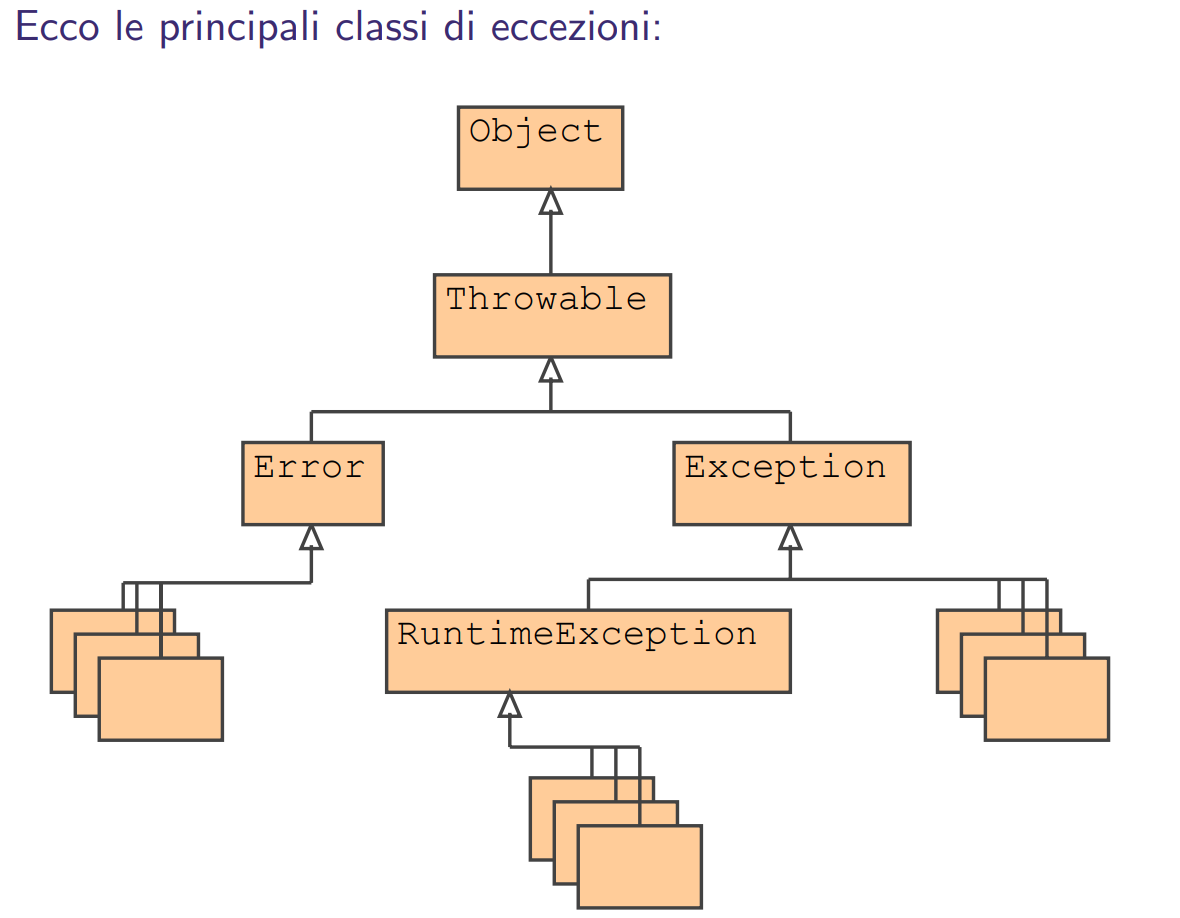
\includegraphics[scale=0.5]{Immagini/eccezioni.png}
\begin{itemize}
    \item La classe \textbf{Throwable} rappresenta tutti gli oggetti che possono
essere lanciati Essa contiene il metodo printStackTrace.
\item La classe \textbf{Error} e le sue sottoclassi rappresentano situazioni
insolite che non sono causate da errori di programmazione o da
ciò che normalmente succede durante l’esecuzione del
programma. Per esempio, la JVM ha esaurito la memoria oppure
qualche altra risorsa non è disponibile.
In genere, una applicazione non è capace di riprendersi da una
situazione di errore. Pertanto, queste eccezioni solitamente non
vengono catturate.
\item La classe \textbf{RuntimeException} rappresenta pure eventi
eccezionali, ma dovuti al programma (errori di programmazione,
bachi). Il programmatore che si accorge di un baco dovuto ad un
suo errore deve correggerlo, non gestirlo! Pertanto, anche queste
eccezioni solitamente non vengono catturate.

\end{itemize}
Una clausola catch (E e) cattura ogni oggetto-eccezione il cui
tipo effettivo è sottotipo di E.
Un’eccezione di tipo effettivo E verrà catturata dal primo blocco
catch in grado di catturarla.

Eventuali eccezioni lanciate dall’interno dei blocchi catch e finally
non vengono catturate dagli altri blocchi catch dello stesso
costrutto.

Se proprio necessario, i try-catch possono essere annidati.

\textbf{L’ordine delle clausole catch è importante.}
Come facciamo a sapere che un metodo può lanciare una
eccezione che dobbiamo catturare?

Così come la dichiarazione del metodo deve specificare il numero
e il tipo dei parametri, il tipo di ritorno, anche le eccezioni che un
metodo può lanciare DEVONO essere dichiarate (a meno che non
siano sottoclassi di Error o di RuntimeException).

La parola chiave throws viene usata per elencare le eccezioni che
possono verificarsi in un metodo.

Il fatto che un metodo dichiara l’eccezione non significa che esso
la lancerà sempre, ma avverte l’utilizzatore che esso potrebbe
lanciarla.
\subsection{Handle or Declare}
Se un metodo non lancia direttamente una eccezione, ma
richiama un altro metodo che può farlo, allora si deve scegliere
almeno una di queste opzioni (regola handle or declare):
\begin{enumerate}
    \item Gestire l’eccezione fornendo le opportune sezioni try/catch
    \item  Dichiarare l’eccezione nell’intestazione del metodo
\end{enumerate}
\textbf{Error} e \textbf{RuntimeException} sono esenti dall’obbligo di dichiarazione.

Esse sono \textbf{unchecked} (non verificate) dal compilatore, mentre le
rimanenti eccezioni sono dette \textbf{checked} (verificate).

Nota: Un metodo può sia gestire che dichiarare eccezioni, una non esclude l'altra.
\subsection{Nuove eccezioni}
È possibile usare tipi di eccezioni già presenti nelle Java API,
oppure crearne di propri in questo modo:

class MiaEccezione extends Exception \{ \}\\\\
Da questo momento in poi si può lanciare un oggetto del tipo
(checked) MiaEccezione.
\section{Java: Regole di overriding}
Posto che sono sovrapponibili solo i metodi visibili della superclasse,
queste sono le regole per l’overriding di metodi:
\begin{itemize}
    \item I due metodi devono avere la stessa firma (nome del metodo
    e tipo dei parametri formali)
    \item Il tipo di ritorno nella sottoclasse può essere uguale o un
    sottotipo del tipo di ritorno originario
    \item Non si può marcare static uno solo dei metodi
    \item Il metodo nella superclasse non può essere marcato final
    \item Il metodo nella sottoclasse deve avere visibilità non inferiore a
    quello della superclasse
    \item Se il metodo nella sottoclasse dichiara di lanciare un tipo di
    eccezione checked, tale tipo deve essere un sottotipo di una delle
    eccezioni dichiarate dal metodo della superclasse
    \item Cioè, le EVENTUALI eccezioni checked dichiarate dal metodo
    nella sottoclasse, DEVONO essere tipi posti al di sotto nella
    gerarchia delle eccezioni dichiarate dal metodo nella superclasse.
\end{itemize}
\section{Java: Classi interne}
Java permette di definire una classe (o interfaccia) all'interno di un'altra.
 
Queste classi vengono chiamate “interne” o “annidate”.
\begin{itemize}
    \item in inglese, il termine usato è nested
    \item In particolare, le classi interne non statiche sono chiamate inner
\end{itemize}
Tale meccanismo arricchisce le possibilità di relazioni tra classi, introducendo in particolare nuove 
regole di visibilità.
\subsection{Proprietà delle classi interne}
Le classi interne (non statiche) godono delle seguenti proprietà distintive:
\begin{enumerate}
    \item \textbf{Privilegi di visibilità} rispetto alla classe contenitrice e alle altre classi in essa contenute premettendo una stretta collaborazione tra queste classi.
    \item \textbf{Restrizione di visibilità} rispetto alle classi esterne a quella contenitrice permettendo di nascondere la classe all'esterno (incapsulamento).
    \item Un \textbf{riferimento implicito} ad un oggetto della classe contenitrice, ovvero ogni oggetto della classe interna “conosce” l'oggetto della classe contenitrice che l'ha creato.

\end{enumerate}
\subsection{Restrizioni di visibilità delle classi interne}
Una classe che non sia interna viene chiamata “top-level”.

A differenza delle classi top-level, le classi interne possono avere \textbf{tutte le quattro visibilità}
ammesse dal linguaggio.

La visibilità di una classe interna X stabilisce quali classi possono utilizzarla (cioè, istanziarla, 
estenderla, dichiarare riferimenti o parametri di tipo X, etc.).

Tra classi contenute nella stessa classe non 
vige alcuna restrizione di visibilità.

Ciascun oggetto di una classe interna (non statica) possiede un \textbf{riferimento 
implicito} ad un oggetto della classe contenitrice.

Tale riferimento viene inizializzato automaticamente al momento della creazione dell'oggetto e non può essere modificato.

Supponiamo che B sia una classe interna di A, allora all'interno della classe B, la sintassi per denotare questo riferimento implicito è \textbf{A.this}.

L'uso di A.this è facoltativo, come quello di this cioè, B può accedere ad un campo o metodo “f” della classe A sia con “A.f” che con “f”.
\subsection{Contesti statici e non}
Il \textbf{contesto statico} di una classe è quella porzione del codice di quella classe che si trova nell’ambito 
di validità di un modificatore static.

Quindi, in una delle seguenti posizioni:
\begin{itemize}
    \item All’interno di un metodo statico
    \item All’interno di un blocco di inizializzazione statico
    \item Nella definizione di un attributo statico
\end{itemize}
La parte restante della classe si chiama \textbf{contesto non statico}.

Supponiamo che B sia una classe interna di A.
Se viene creato un oggetto di tipo B in un contesto non statico della classe A, il riferimento implicito 
verrà inizializzato con il valore corrente di this.

In tutti gli altri casi, è necessario utilizzare una nuova forma dell'operatore “new”, ovvero:

A a = new A();

B b = a.new B(); // new è preceduto dal riferimento della classe A
\subsection{Classi interne statiche}
Le classi interne possono essere statiche o meno.

Una classe interna dichiarata nello scope di classe (cioè al di fuori di metodi e inizializzatori) è statica 
se preceduta dal modificatore “static”.

Le classi interne possono anche trovarsi all'interno di un metodo \textbf{classi locali}, non affrontate in questo corso.

Le classi interne statiche \textbf{non possiedono il riferimento implicito} alla classe contenitrice.
Le classi interne statiche \textbf{godo delle stesse proprietà di quelle non statiche a meno del  riferimento implicito}.\\
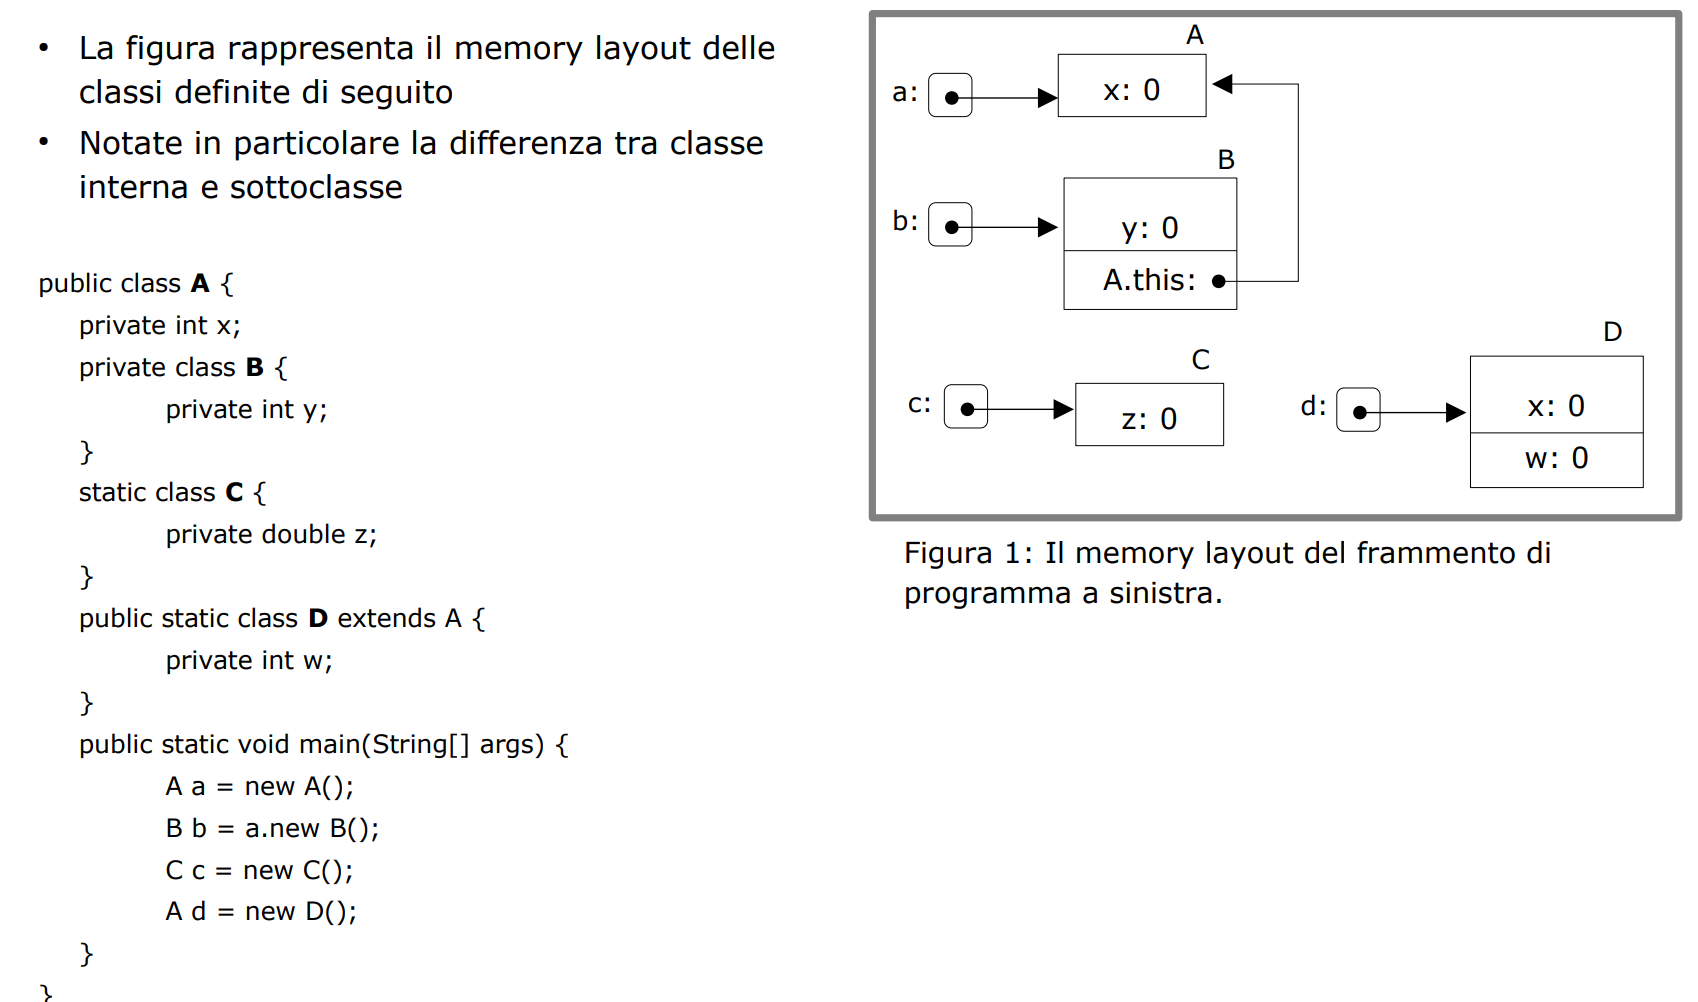
\includegraphics[scale=0.6]{Immagini/classi_interne.png}
\section{Java: Costruttori di oggetti}
\subsection{Elementi sintattici}
\begin{itemize}
    \item I costruttori (metodi col nome della classe e senza tipo di ritorno)
    \item Invocazioni da un costruttore a un altro (this e super)
    \item I blocchi di inizializzazione (blocchi di codice anonimi nello scope di classe)
    \item Gli inizializzatori. Es. private int n = $<exp>$;
\end{itemize}
\subsection{Concatenazione dei costruttori}
Il meccanismo tramite il quale i costruttori possono invocarsi a vicenda prende il nome di 
concatenazione dei costruttori (constructor chaining).
\subsubsection{Invocazioni esplicite ad un altro costruttore}
Un costruttore può chiamarne un altro della stessa classe usando la parola chiave \textbf{this}, oppure un costruttore 
della sua superclasse diretta usando la parola chiave \textbf{super}.


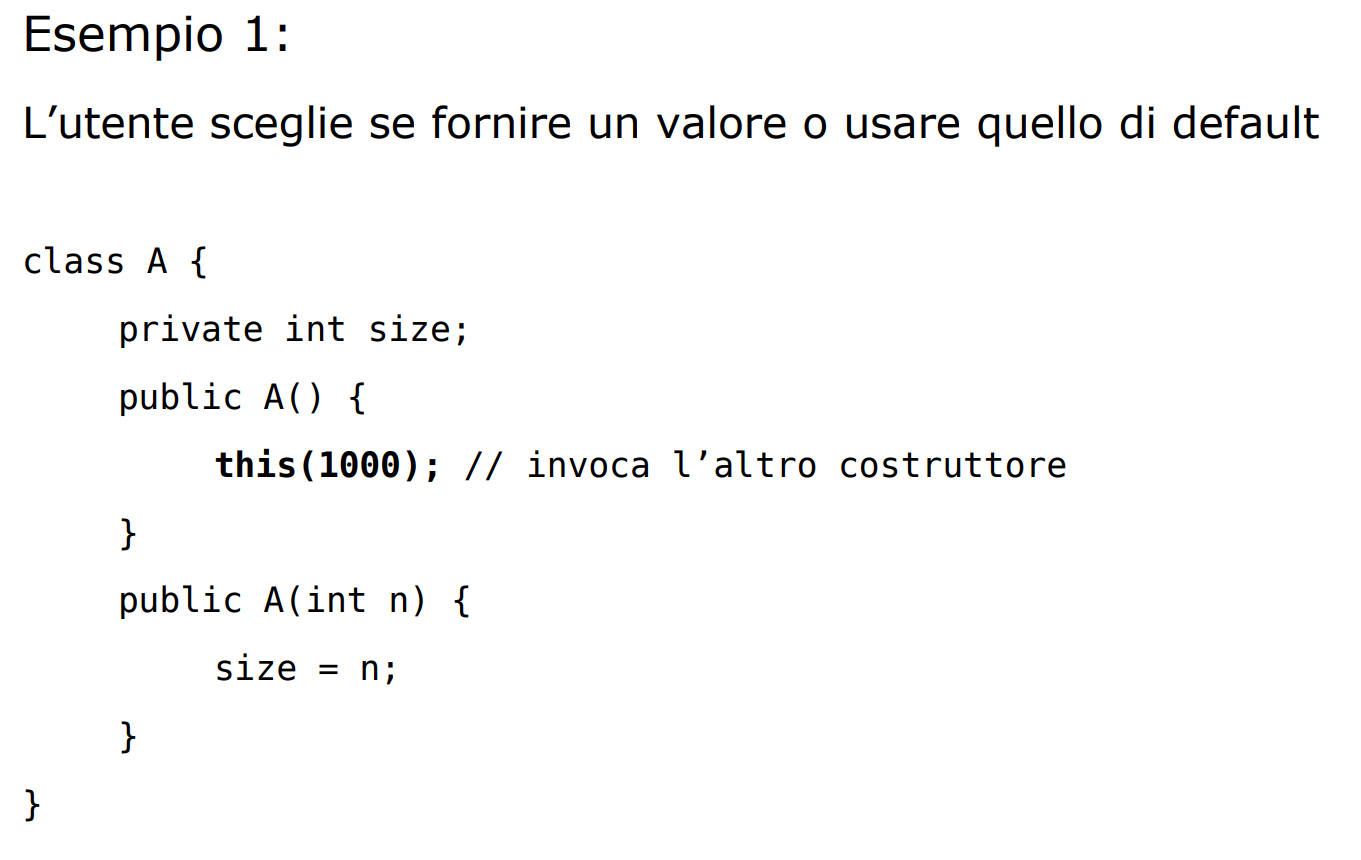
\includegraphics[scale=0.4]{Immagini/es1_costruttori.png}
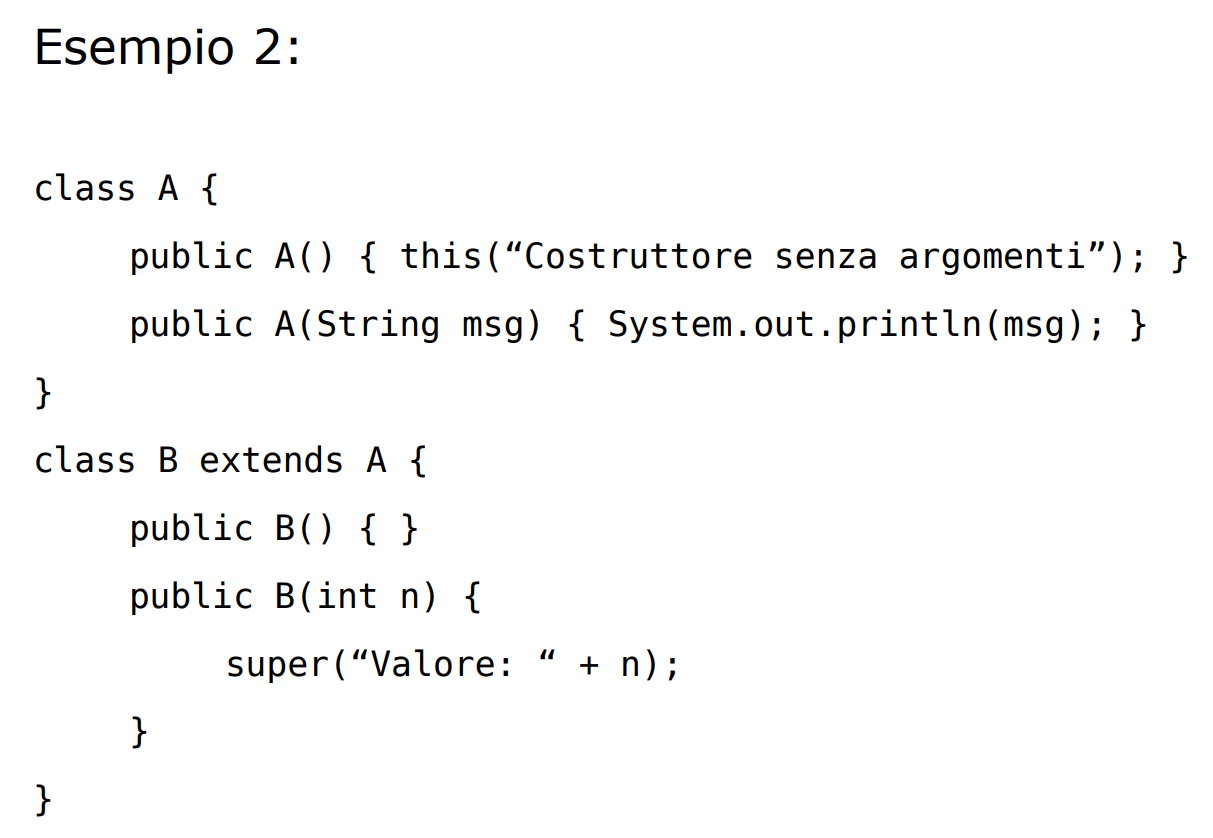
\includegraphics[scale=0.4]{Immagini/es2_costruttori.png}
\subsubsection{Chiamate implicite ad un altro costruttore}
Se un costruttore \textbf{non inizia} con una chiamata ad un altro costruttore (this o super), il compilatore inserisce 
\textbf{automaticamente} una chiamata al costruttore senza argomenti della superclasse ovvero, inserisce l’istruzione “super()”.

In tal caso, se la superclasse non ha un costruttore senza argomenti, si verifica un errore di compilazione.
\subsection{Sequenza di inizializzazione di un oggetto}
\begin{enumerate}
    \item \begin{enumerate}
        \item Se il costruttore inizia con super(…), passare al costruttore della superclasse (risoluzione overloading)
        \item Se il costruttore inizia con this(…), passare al costruttore indicato (risoluzione overloading)
        \item Se il costruttore non inizia né con super né con this, passare al costruttore senza argomenti della 
        superclasse (a meno di non essere in Object)
    \end{enumerate}
    \item Eseguire i blocchi di inizializzazione e gli inizializzatori degli attributi, nell’ordine in cui compaiono nel codice
    \item Eseguire il resto del costruttore
\end{enumerate}
Nota 1: un attributo privo di inizializzatore assume il valore di default del suo tipo.\\
Nota 2: un blocco di inizializzazione o un inizializzatore non può fare riferimento a un attributo la cui 
dichiarazione non segue lessicalmente tale blocco o inizializzatore (errore di compilazione).
\subsection{Concatenazione ciclica}
Il compilatore controlla che la concatenazione \textbf{non sia ciclica}.

Infatti, se dei costruttori si chiamano a vicenda, siccome tali chiamate si trovano alla prima riga del 
rispettivo costruttore, e pertanto avvengono incondizionatamente, ci si trova in presenza di una 
mutua ricorsione non ben fondata, ovvero infinita.

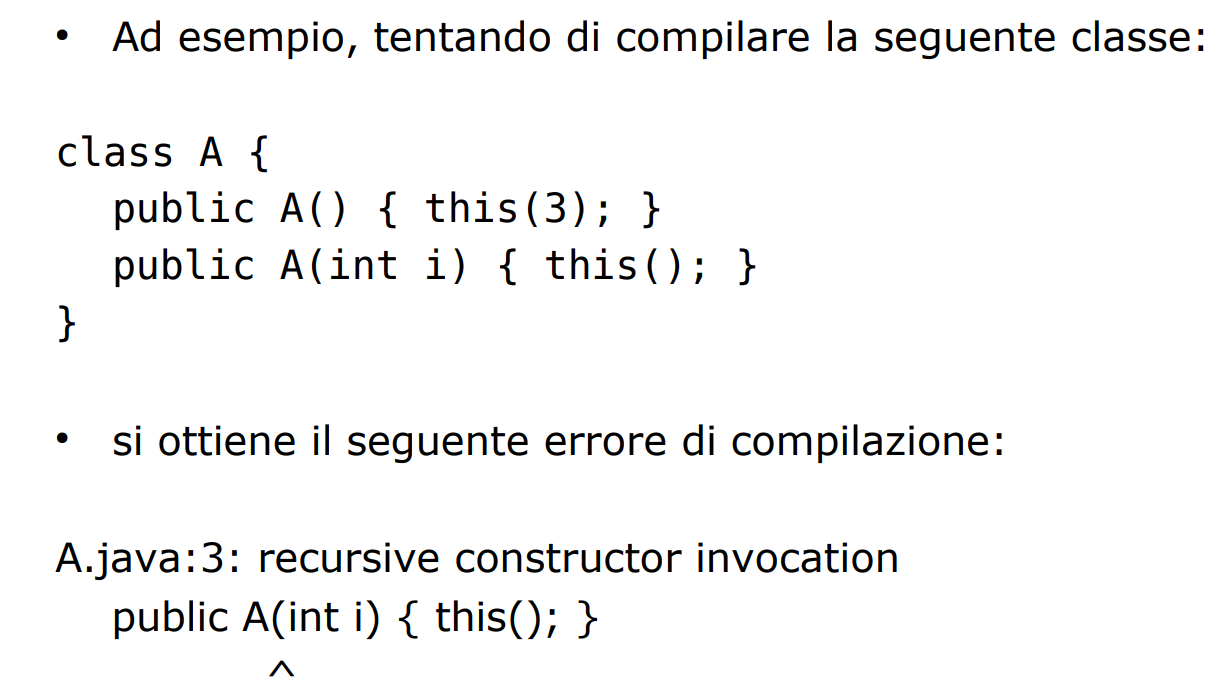
\includegraphics[scale=0.5]{Immagini/Concatenazione_ciclica.png}

Per analizzare la concatenazione dei costruttori di una data gerarchia di classi, ed in particolare 
controllare che essa non sia ciclica, è possibile realizzare il seguente diagramma:
\begin{enumerate}
    \item Creare un grafo con un nodo per ogni costruttore, compresi quelli impliciti
    \item Aggiungere un arco da un nodo x ad un nodo y se il costruttore x chiama, esplicitamente o 
meno, il costruttore y
    \item l grafo ottenuto non deve presentare cicli
\end{enumerate}
\section{Java: Polimorfismo}
Definizione: Uno stesso oggetto sintattico (funzione, 
metodo, variabile, etc.) appartiene a più tipi.\\\\
Esempio: operatore + in Java

1 + 2 ha un tipo e un significato diverso da “a” + “b”.

\begin{itemize}
    \item Ad hoc
    \begin{itemize}
        \item Specifico per particolari tipi di dato
    \end{itemize}
    \item Universale
    \begin{itemize}
        \item Si applica ad un numero di casi illimitato
        \item Ad es. aggiungendo una nuova superclasse con un metodo 
        concreto, l'overriding crea casi di polimorfismo rispetto a 
        tutte le sottoclassi che già definiscono quel metodo
    \end{itemize}
\end{itemize}
\subsection{Polimorfismo ad hoc}
\begin{itemize}
    \item Overloading
    \begin{itemize}
        \item stesso nome ma diversa implementazione a seconda dei tipi dei parametri
    \end{itemize}
    \item Coercion
    \begin{itemize}
        \item promozione automatica dei tipo
    \end{itemize}
\end{itemize}
\subsection{Polimorfismo universale}
\begin{itemize}
    \item Per inclusione (o di sottotipo")
    \begin{itemize}
        \item overriding nelle sottoclassi
    \end{itemize}
    \item Parametrico
    \begin{itemize}
        \item tipi parametrici, generics o templates
    \end{itemize}
\end{itemize}
\section{Linguaggi Funzionali - ML}
ML è fortemente e staticamente tipato.
Il controllo dei tipi avviene interamente a tempo di
compilazione, ma non richiede di dichiarare il tipo degli identificatori (spesso lo capisce da solo \textbf{type inference}).

Usa sia \textbf{structural equivalence} sia \textbf{name equivalence}.
Permette di definire tipi ricorsivi (liste, alberi, ...).
Supporta polimorfismo parametrico (come i template).
Supporta encapsulation (tipi di dato astratti) ma non è un
linguaggio a oggetti.
Mancano la gerarchia di tipi e di conseguenza l’ereditarietà.
\\\\
Con val si aggiunge un nuovo identificatore all’ambiente e gli si
associa un valore.

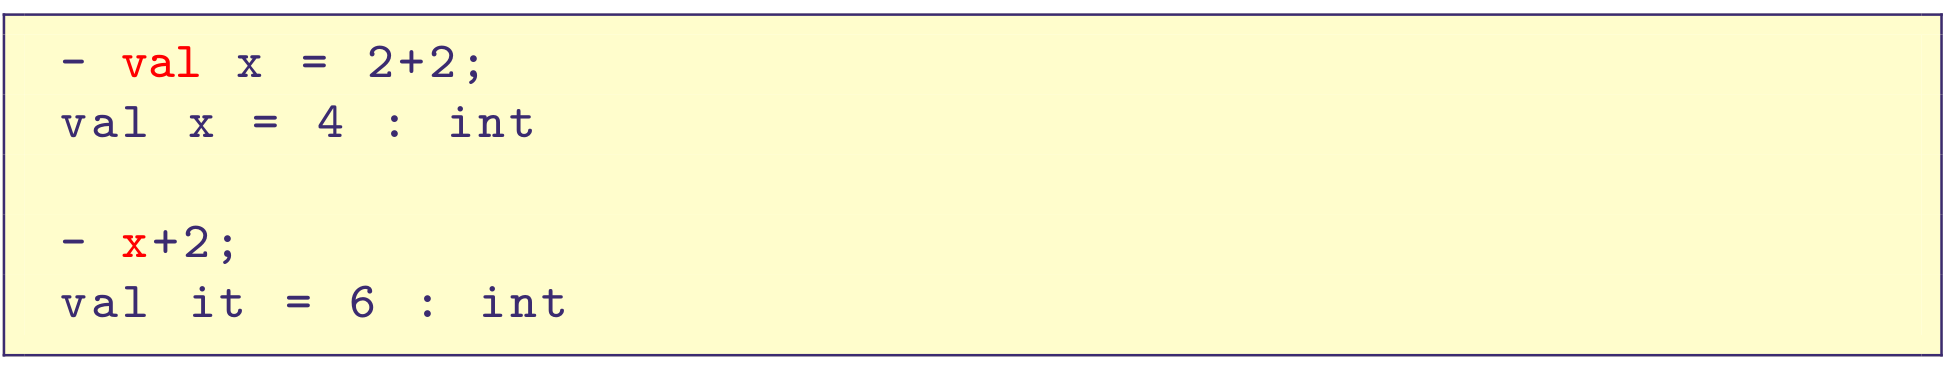
\includegraphics[scale=0.2]{Immagini/ml4.png}
\subsection{Funzioni}
Ci sono diversi modi di definire e chiamare funzioni in ML.

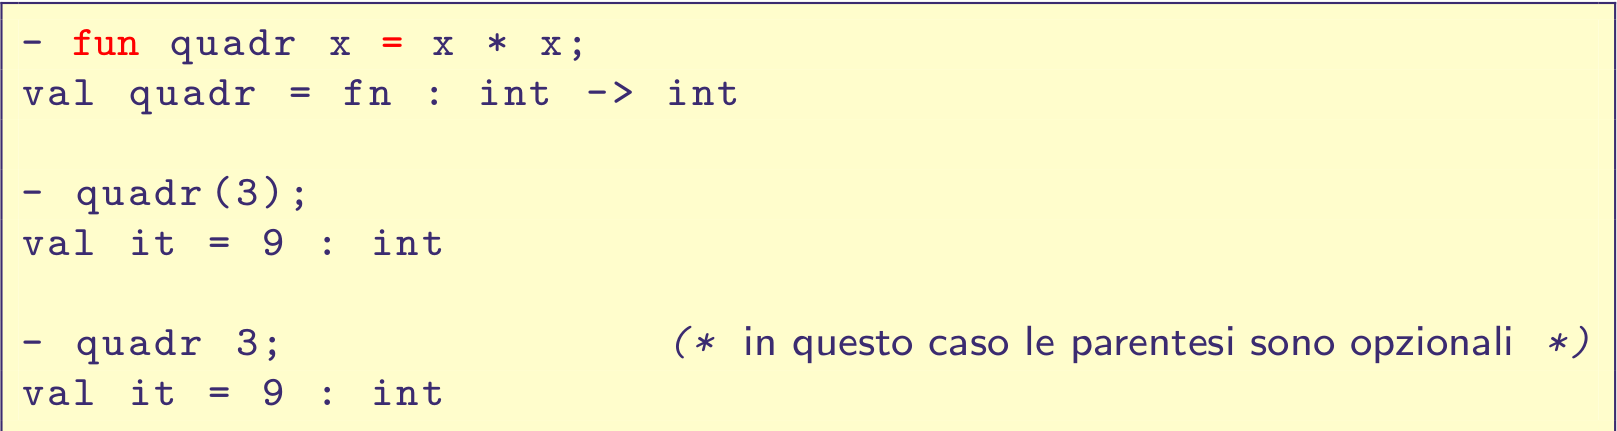
\includegraphics[scale=0.2]{Immagini/ml1.png}
\\
Con \textbf{fun} si dichiara la funzione;
fun aggiunge all’ambiente l’identificatore quadr
e lo associa alla funzione da interi a interi.
\\\\
È possibile indicare esplicitamente i tipi:

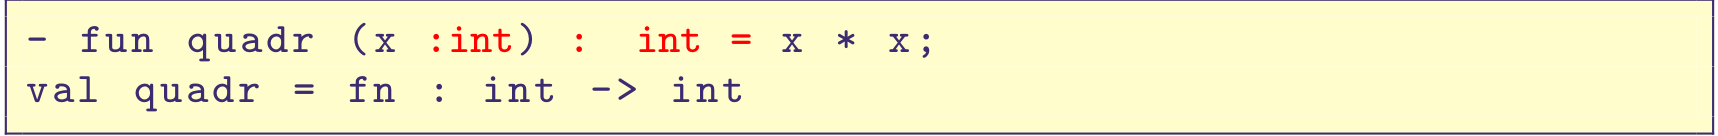
\includegraphics[scale=0.2]{Immagini/ml2.png}
\\
In assenza di annotazioni di tipo, scatta la type inference.
\\\\
In ML il costrutto if-then-else denota un’espressione.

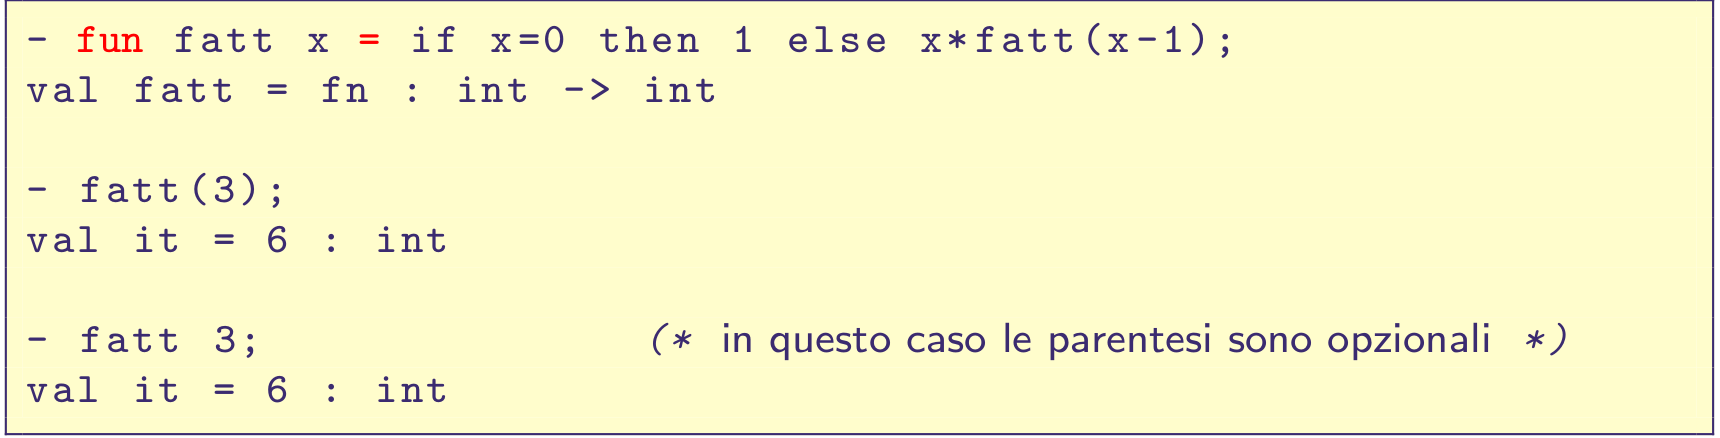
\includegraphics[scale=0.2]{Immagini/ml3.png}
\subsection{Scoping}
L’equivalente dei blocchi in ML è

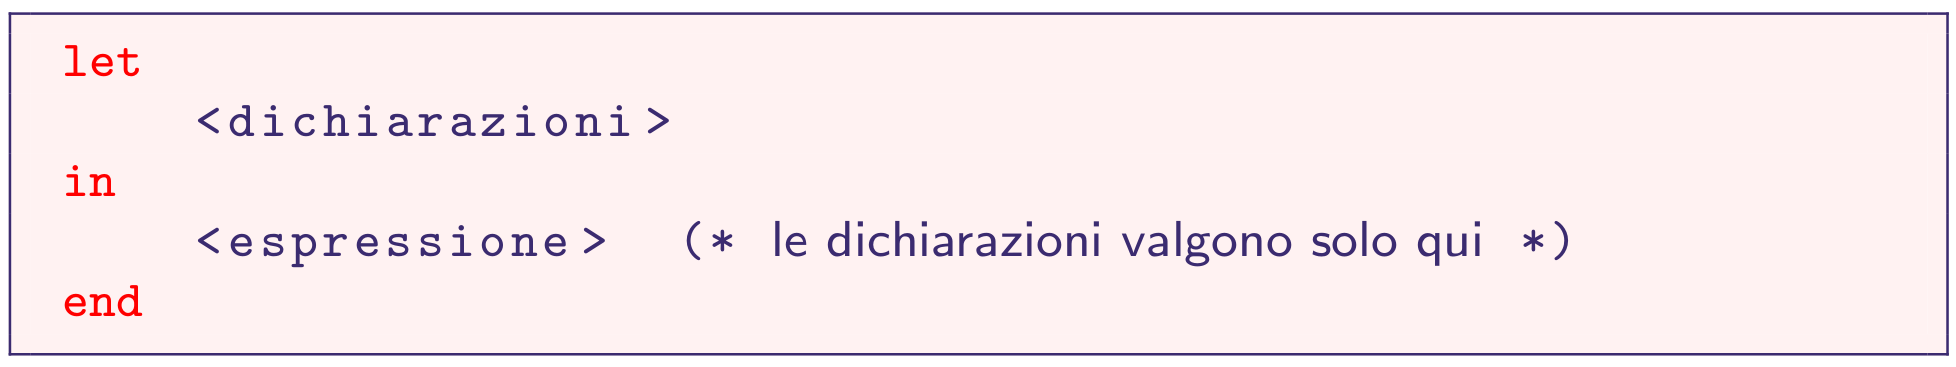
\includegraphics[scale=0.2]{Immagini/ml5.png}

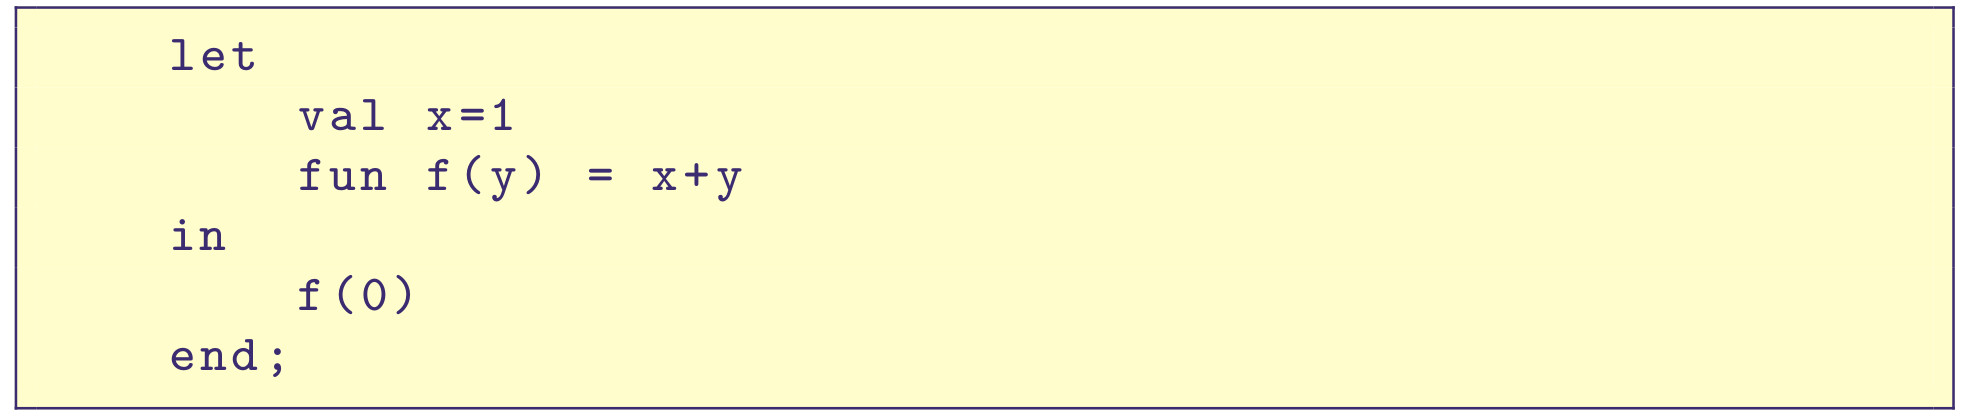
\includegraphics[scale=0.2]{Immagini/ml6.png}
\\\\
Simile a let ma dopo in c’è una dichiarazione invece di una
espressione da valutare

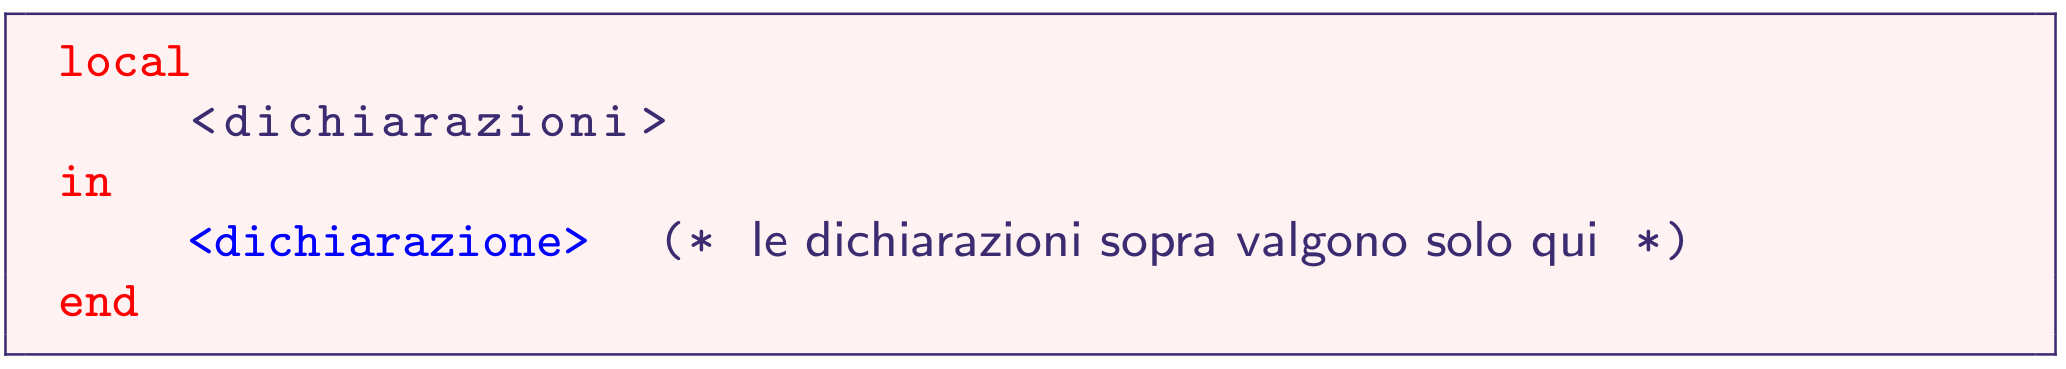
\includegraphics[scale=0.2]{Immagini/ml7.png}
\subsection{Prodotti cartesiani}
\begin{itemize}
    \item Si possono definire n-uple semplicemente mettendo i valori tra
parentesi
\item Il prodotto cartesiano viene indicato con ‘*’
\item Si estrae l’i-esimo elemento da una n-upla con l’operatore
prefisso \#i
\end{itemize}
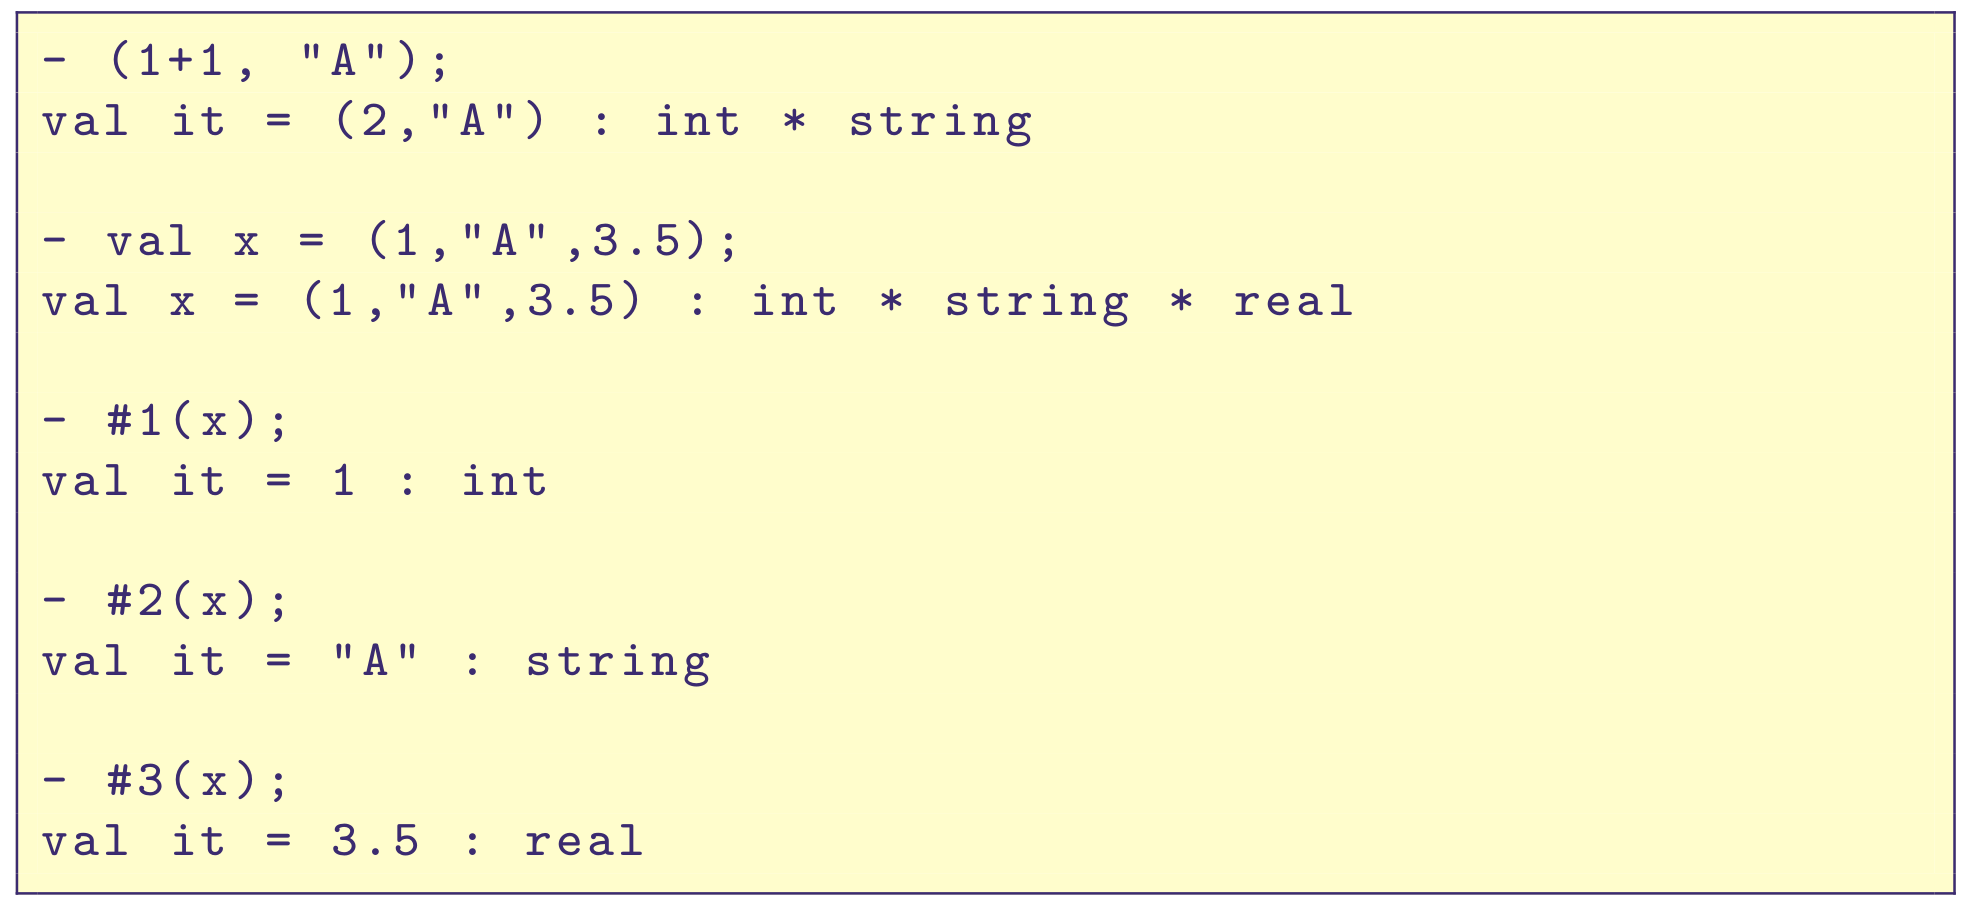
\includegraphics[scale=0.2]{Immagini/ml8.png}
\subsection{Record}
Insiemi di espressioni $<nome>=<valore>$. Da notare come viene
rappresentato il tipo.

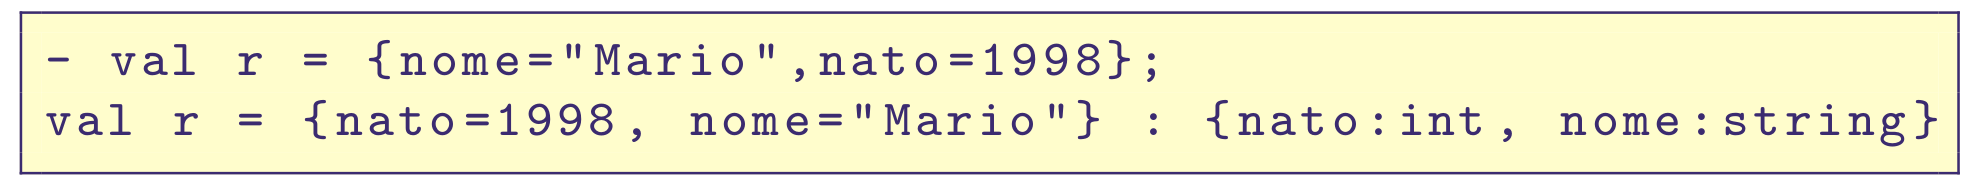
\includegraphics[scale=0.2]{Immagini/ml9.png}
\\\\
Il valore associato al nome N si estrae con \#N.

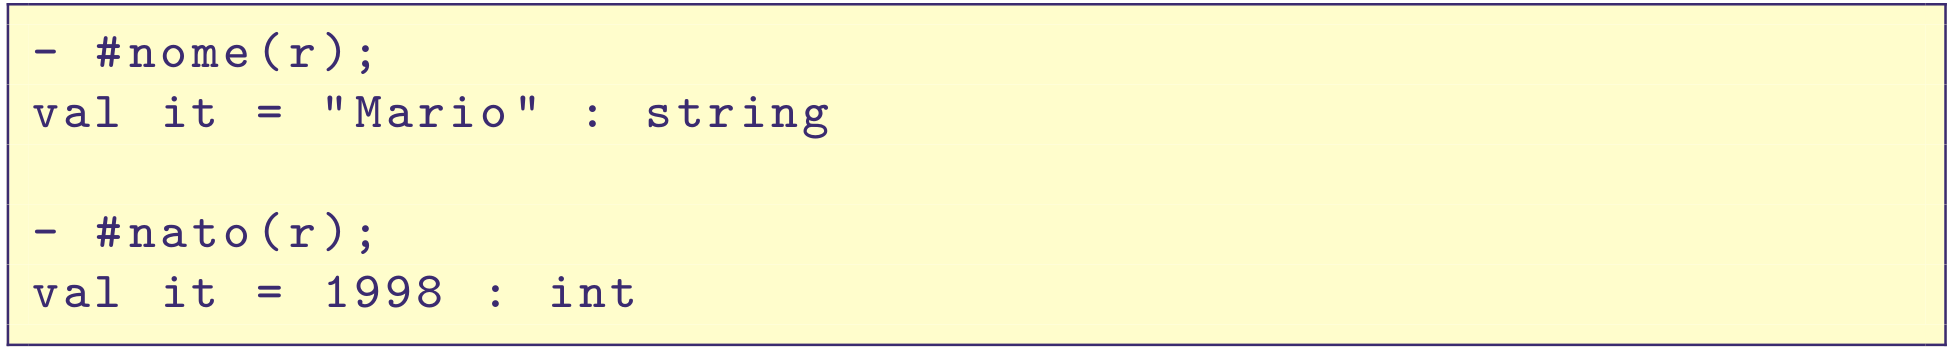
\includegraphics[scale=0.2]{Immagini/ml10.png}
\\\\
L’ordine delle coppie non conta.

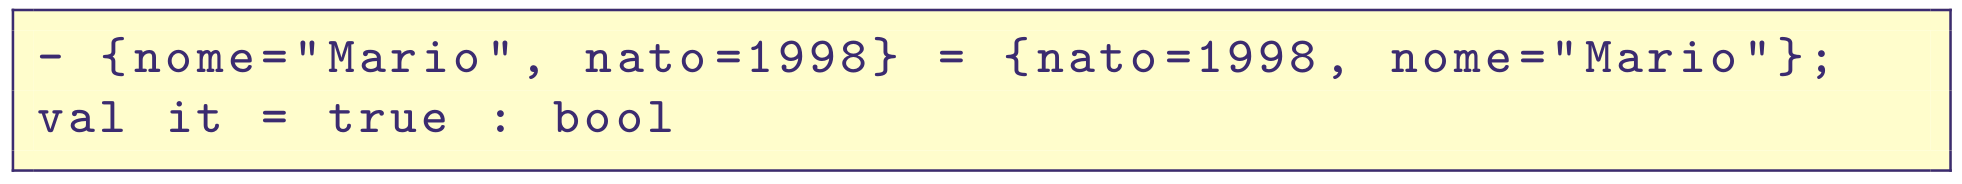
\includegraphics[scale=0.2]{Immagini/ml11.png}
\subsection{Dichiarazioni di tipo}
ML permette di definire nuovi tipi similmente ai typedef del C.

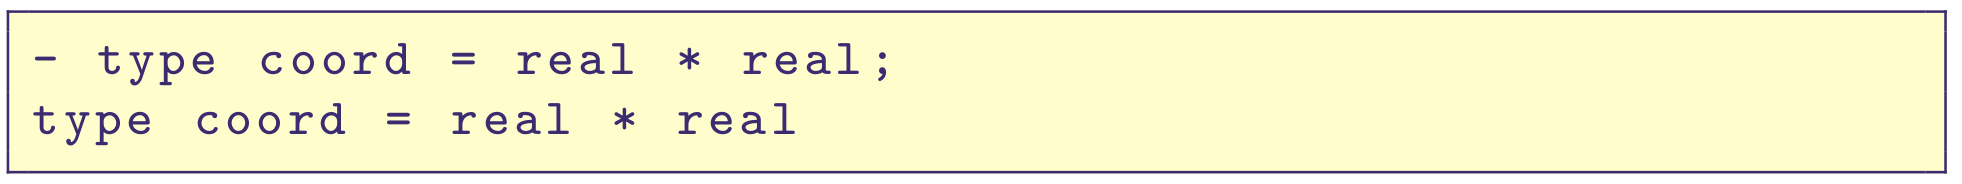
\includegraphics[scale=0.2]{Immagini/ml12.png}
\\\\
Il compilatore va aiutato a stabilire il tipo.

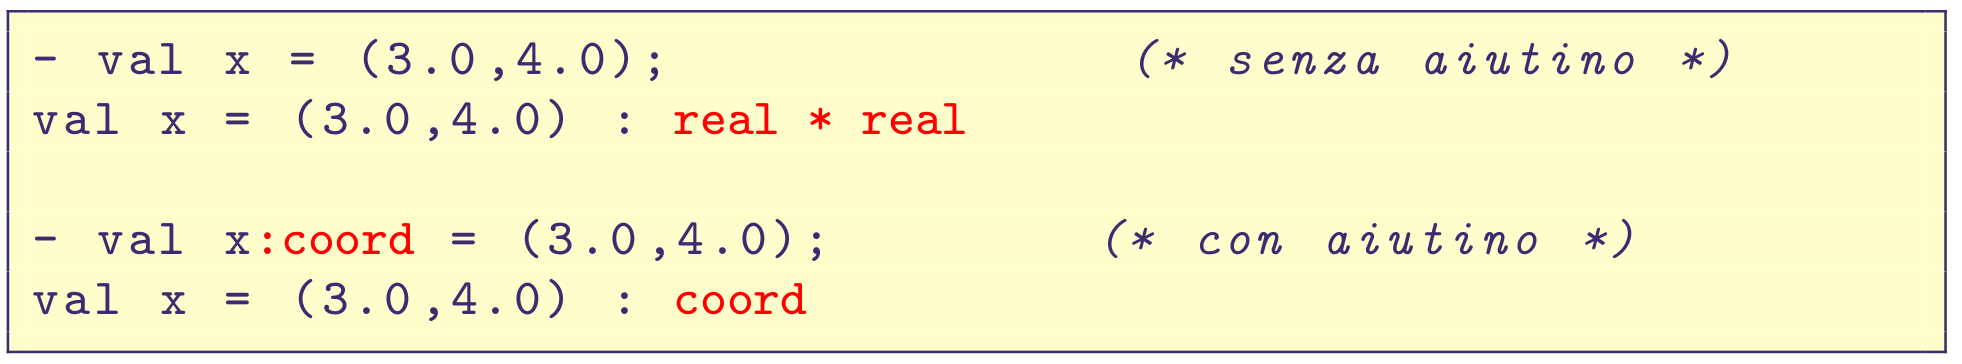
\includegraphics[scale=0.2]{Immagini/ml13.png}
\\\\
I tipi coord e (real * real) sono compatibili tra loro
(structural equivalence).

Posso passare una espressione di tipo coord a un parametro
di tipo (real * real) e viceversa.
\subsection{Datatypes e costruttori}
Con datatype si può fare di più che dare un nome a un tipo ML.

Si possono definire \textbf{costruttori} per creare data objects.

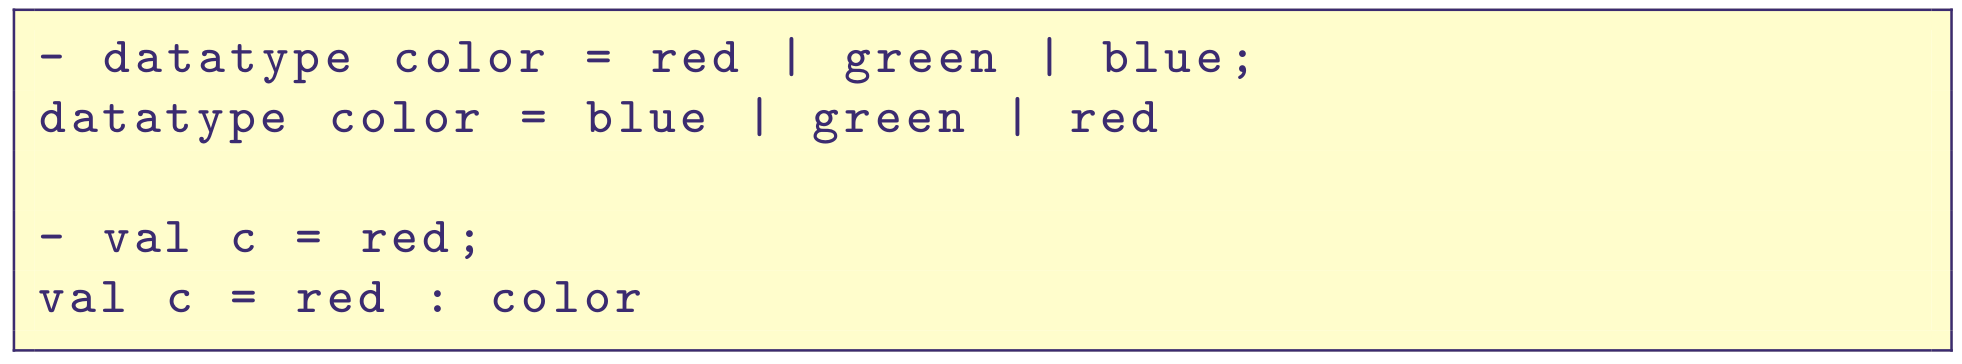
\includegraphics[scale=0.2]{Immagini/ml14.png}
\\\\
red, green, blue sono costruttori. Definiscono i possibili
valori del tipo color e sono oggetti completamente nuovi.

Ogni tipo definito con datatype è incompatibile con tutti gli
altri tipi (name equivalence).
\\\\
\subsubsection{Un esempio: definire una lista concatenata di interi}
\begin{itemize}
    \item Se ne può dare una definizione ricorsiva:
    \begin{itemize}
        \item lista vuota (caso base)
        \item nodo che contiene un intero ed una lista di interi (caso induttivo)
    \end{itemize}
\end{itemize}
Quindi servono 2 costruttori: per la lista vuota e per i nodi.

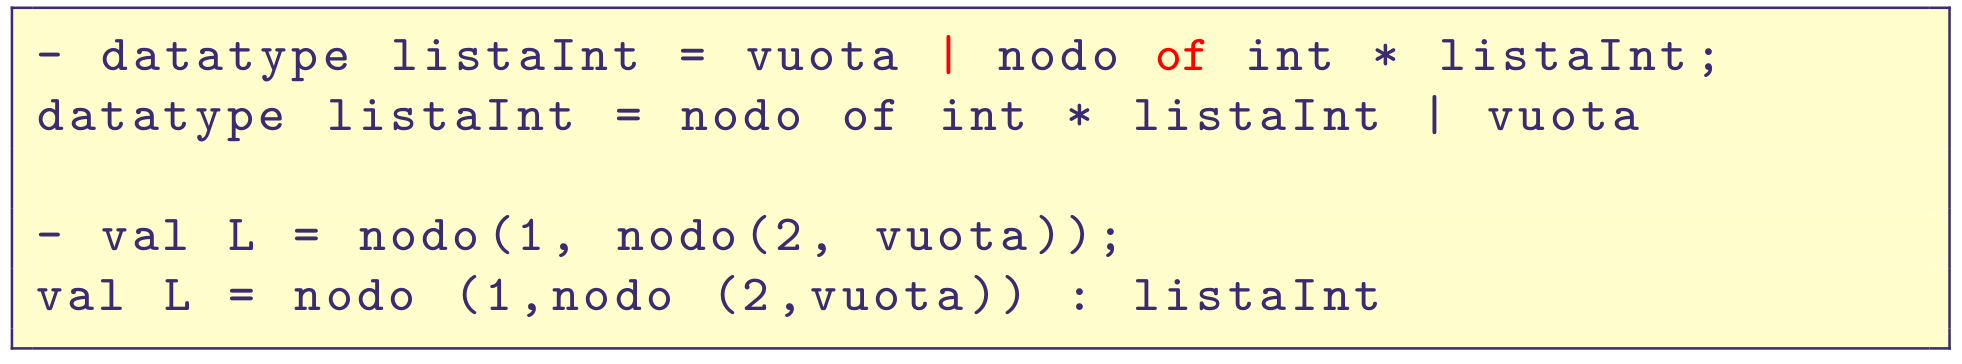
\includegraphics[scale=0.2]{Immagini/ml15.png}
\\\\
\subsubsection{Altro esempio: albero binario con nodi etichettati da interi}
\begin{itemize}
    \item Definizione ricorsiva
    \begin{itemize}
        \item albero vuoto, oppure
        \item nodo che contiene un intero e due alberi dello stesso tipo
    \end{itemize}
\end{itemize}
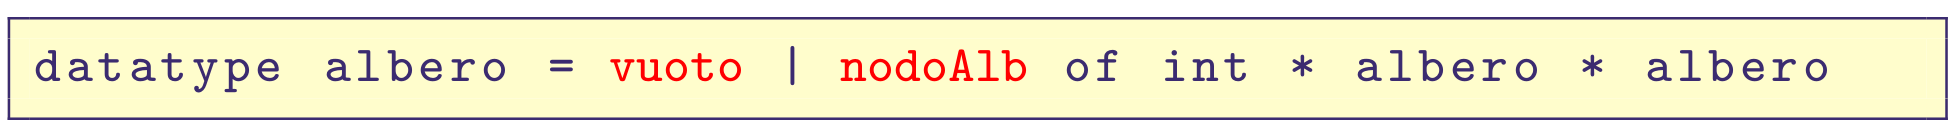
\includegraphics[scale=0.2]{Immagini/ml16.png}
\\\\
In questo esempio costruiamo un albero con radice 1, figlio
sinistro 2 (che è una foglia), mentre il figlio destro manca.

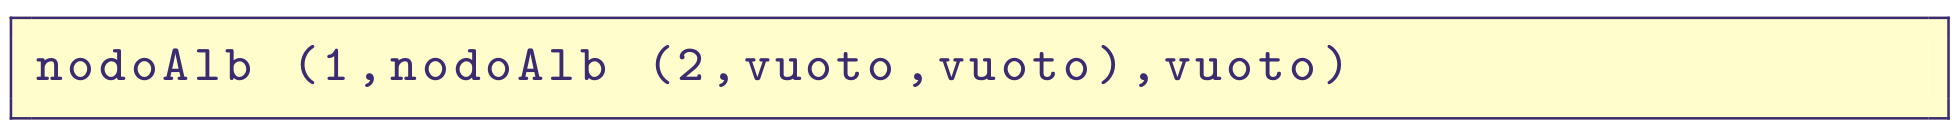
\includegraphics[scale=0.2]{Immagini/ml17.png}
\subsection{Patterns e matching}
Per scandire una lista abbiamo innanzitutto bisogno di controllare
se è vuota.

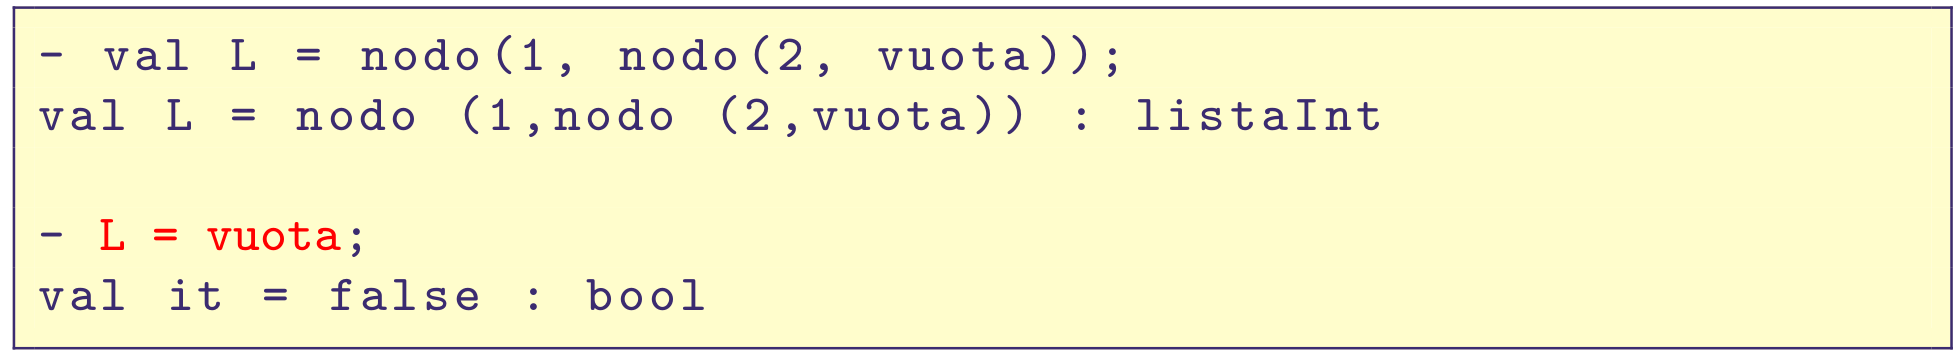
\includegraphics[scale=0.2]{Immagini/ml18.png}
\\\\
Se non è vuota potrebbe servirci il primo elemento. Si estrae con
pattern matching.

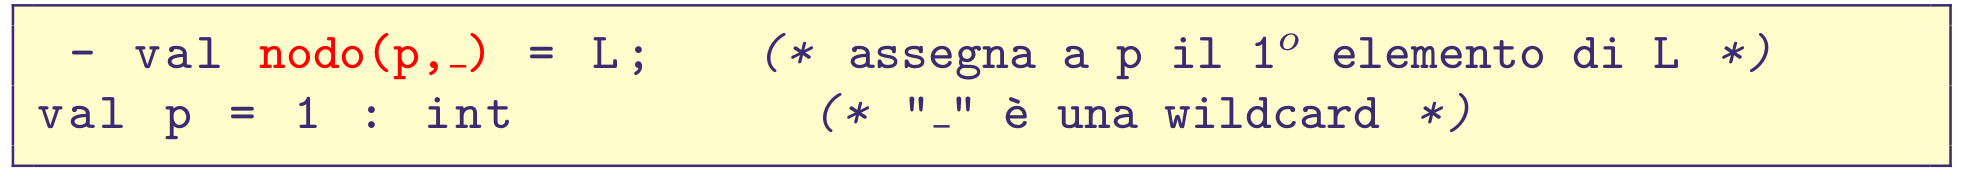
\includegraphics[scale=0.2]{Immagini/ml19.png}
\\\\
La parte in rosso è chiamata pattern.
\\\\
Per ottenere il resto della lista.

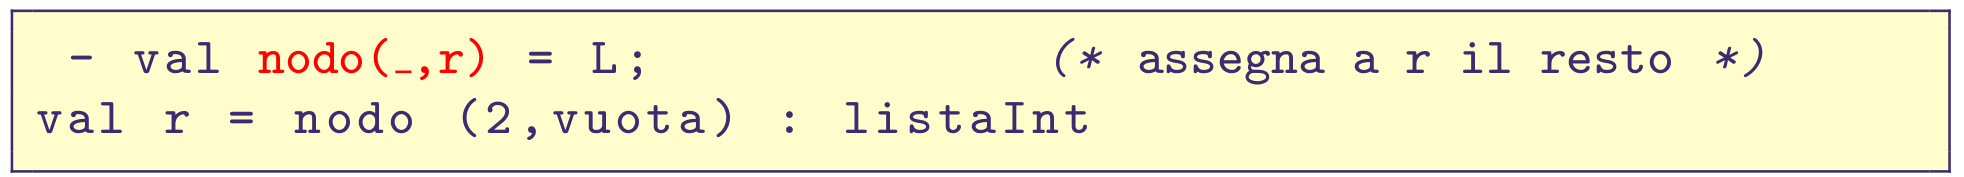
\includegraphics[scale=0.2]{Immagini/ml20.png}
\subsubsection{Funzione che conta gli elementi della lista}
Ovviamente deve essere ricorsiva (niente cicli!)

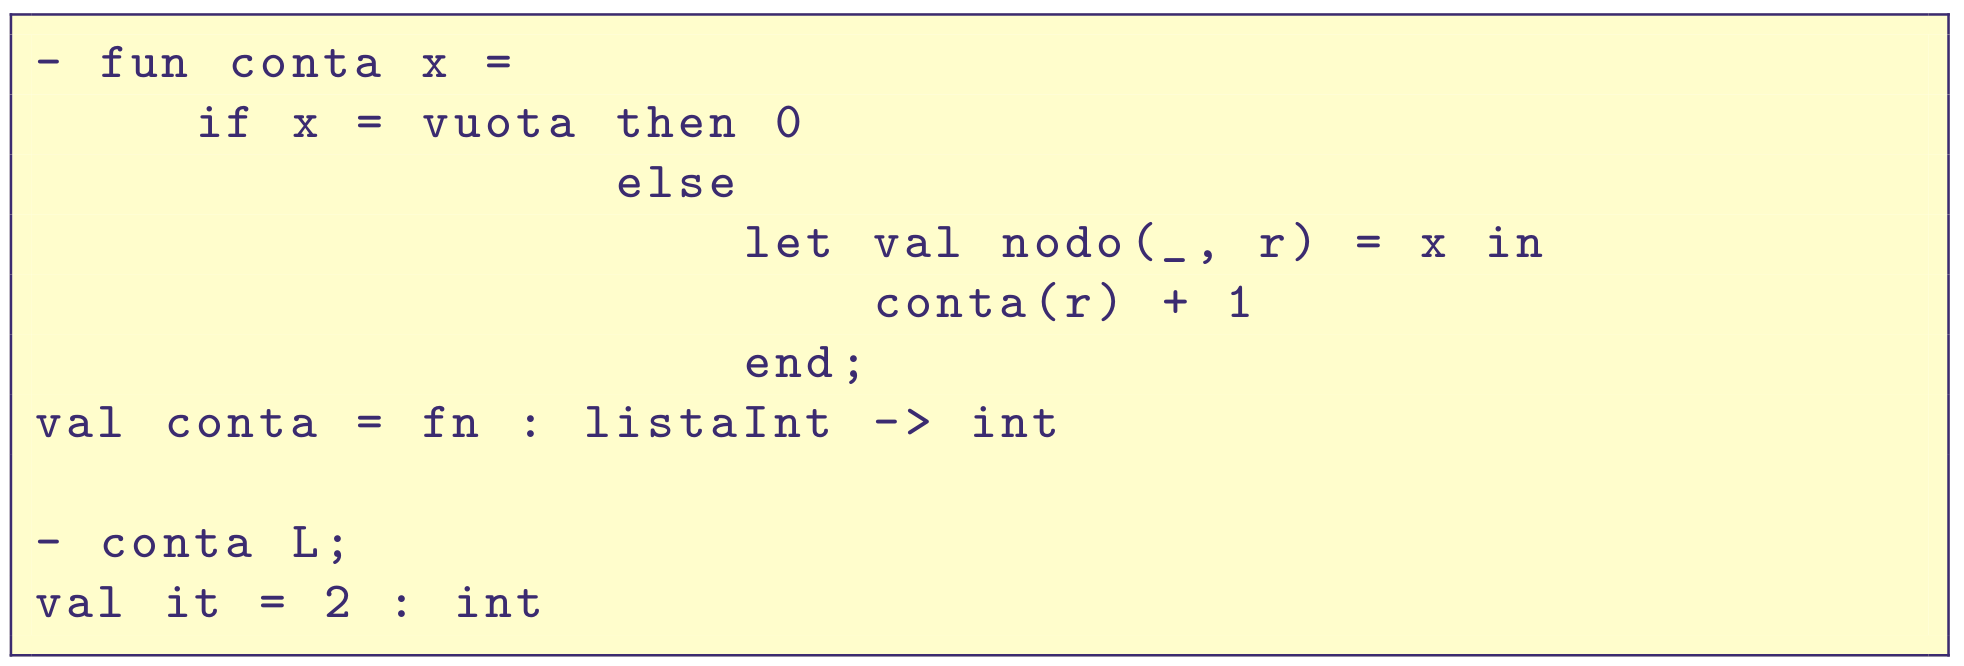
\includegraphics[scale=0.2]{Immagini/ml21.png}
\\\\
Notare come il compilatore ha inferito il tipo della funzione.
\begin{itemize}
    \item x viene confrontato con “vuota”, che è di tipo listaInt $->$ anche x è
di tipo listaInt $->$ l’input di “conta” è un listaInt
\item il “then” restituisce 0, che è un intero; quindi l’output di “conta” è
un intero
\end{itemize}
Inoltre il compilatore controlla che anche il resto della funzione
sia compatibile con questi tipi.
\begin{itemize}
    \item r corrisponde al 2° argomento del nodo, che è di tipo listaInt $->$ è
corretto passarlo a conta che restituisce un intero
\item il “then” restituisce 0, che è un intero; quindi l’output di “conta” è
un intero
\end{itemize}
Si possono estrarre tutti gli elementi di un costruttore in un colpo solo

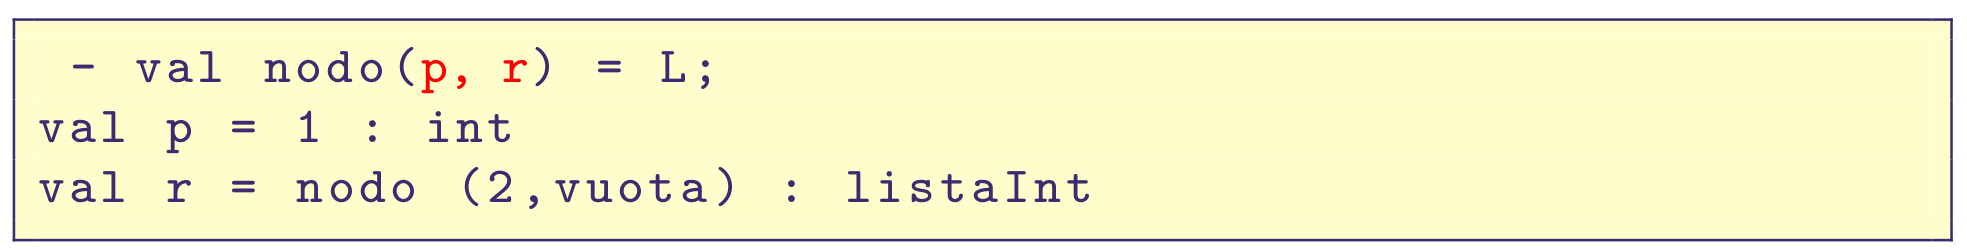
\includegraphics[scale=0.2]{Immagini/ml22.png}
\\\\
Cioè dichiara due identificatori (p e r) in un colpo solo
\subsubsection{Funzione per casi}
Si può definire una funzione per casi mettendo direttamente i pattern al posto dei parametri formali

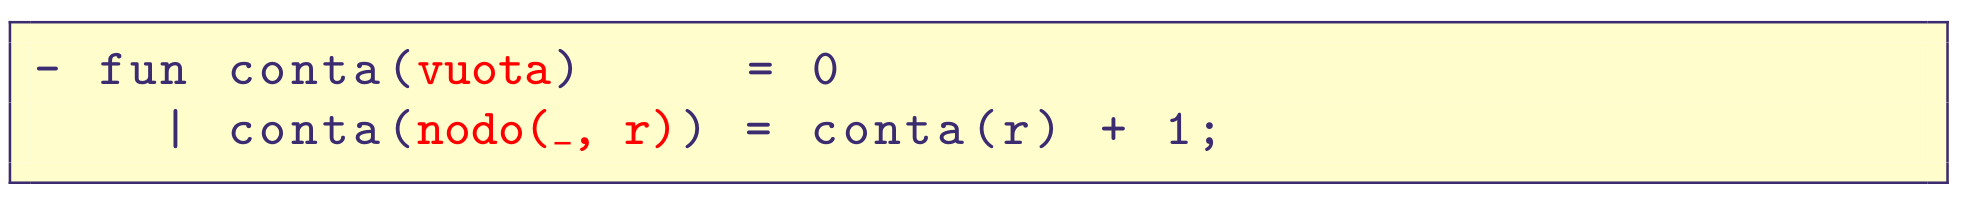
\includegraphics[scale=0.2]{Immagini/ml23.png}
\\\\
Oppure in modo analogo allo switch/case del C.
L’idea è la stessa della definizione per casi delle funzioni.

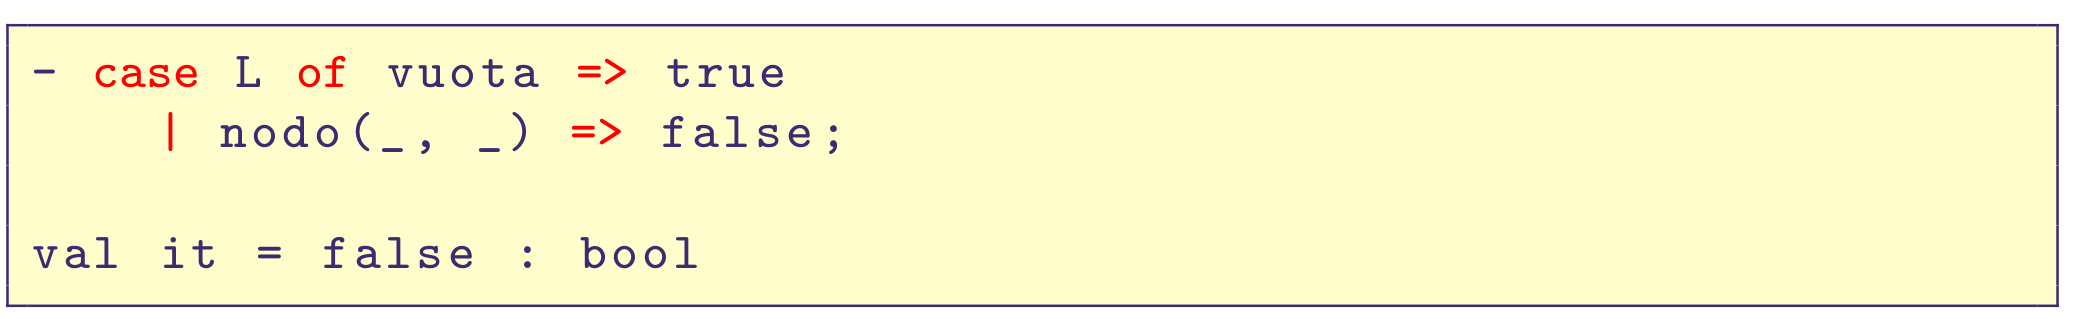
\includegraphics[scale=0.2]{Immagini/ml24.png}
\subsection{Liste}
Le liste sono tra le strutture dati più usate in programmazione
funzionale; in qualche misura sostituiscono i vettori (concetto
essenzialmente imperativo).
Perciò ML le fornisce built-in con i costruttori nil e ::

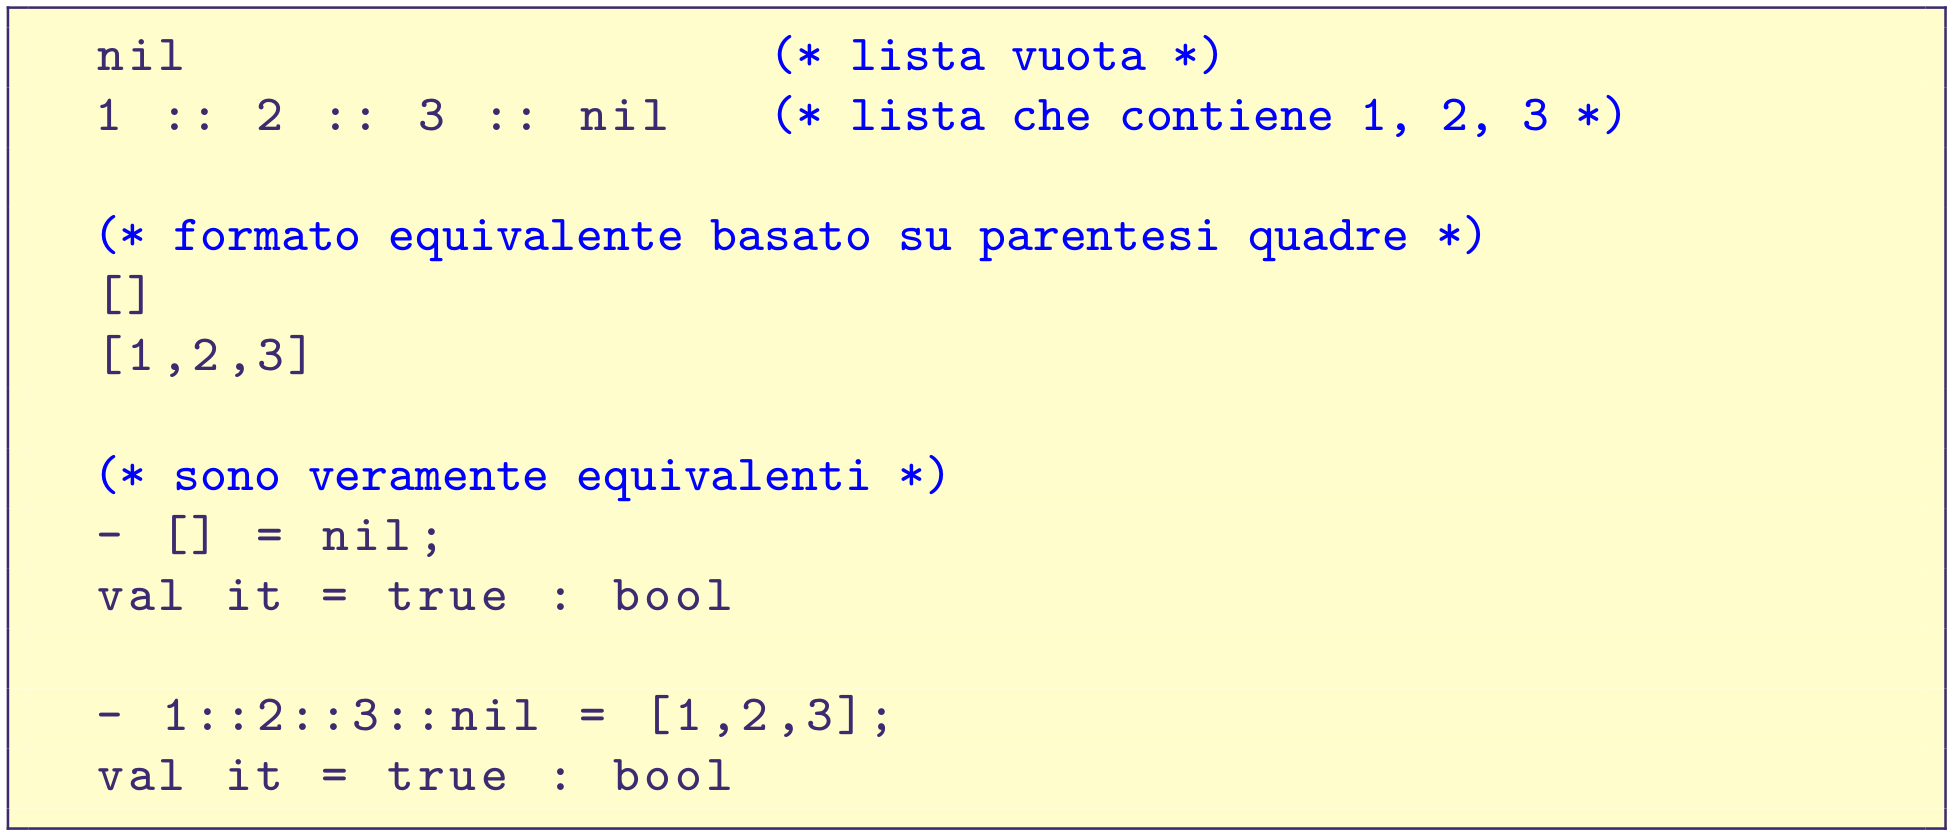
\includegraphics[scale=0.2]{Immagini/ml25.png}
\subsubsection{Principali operatori sulle liste in ML}
\begin{itemize}
    \item La funzione \textbf{length} restituisce la lunghezza di una lista
    \item La funzione \textbf{null} restituisce true se la lista è vuota
    \item Le funzioni \textbf{hd} (head) e \textbf{tl} (tail) restituiscono il primo elemento e il resto della lista, rispettivamente
    \item L’operatore infisso \textbf{@} restituisce la concatenazione di due liste
\end{itemize}
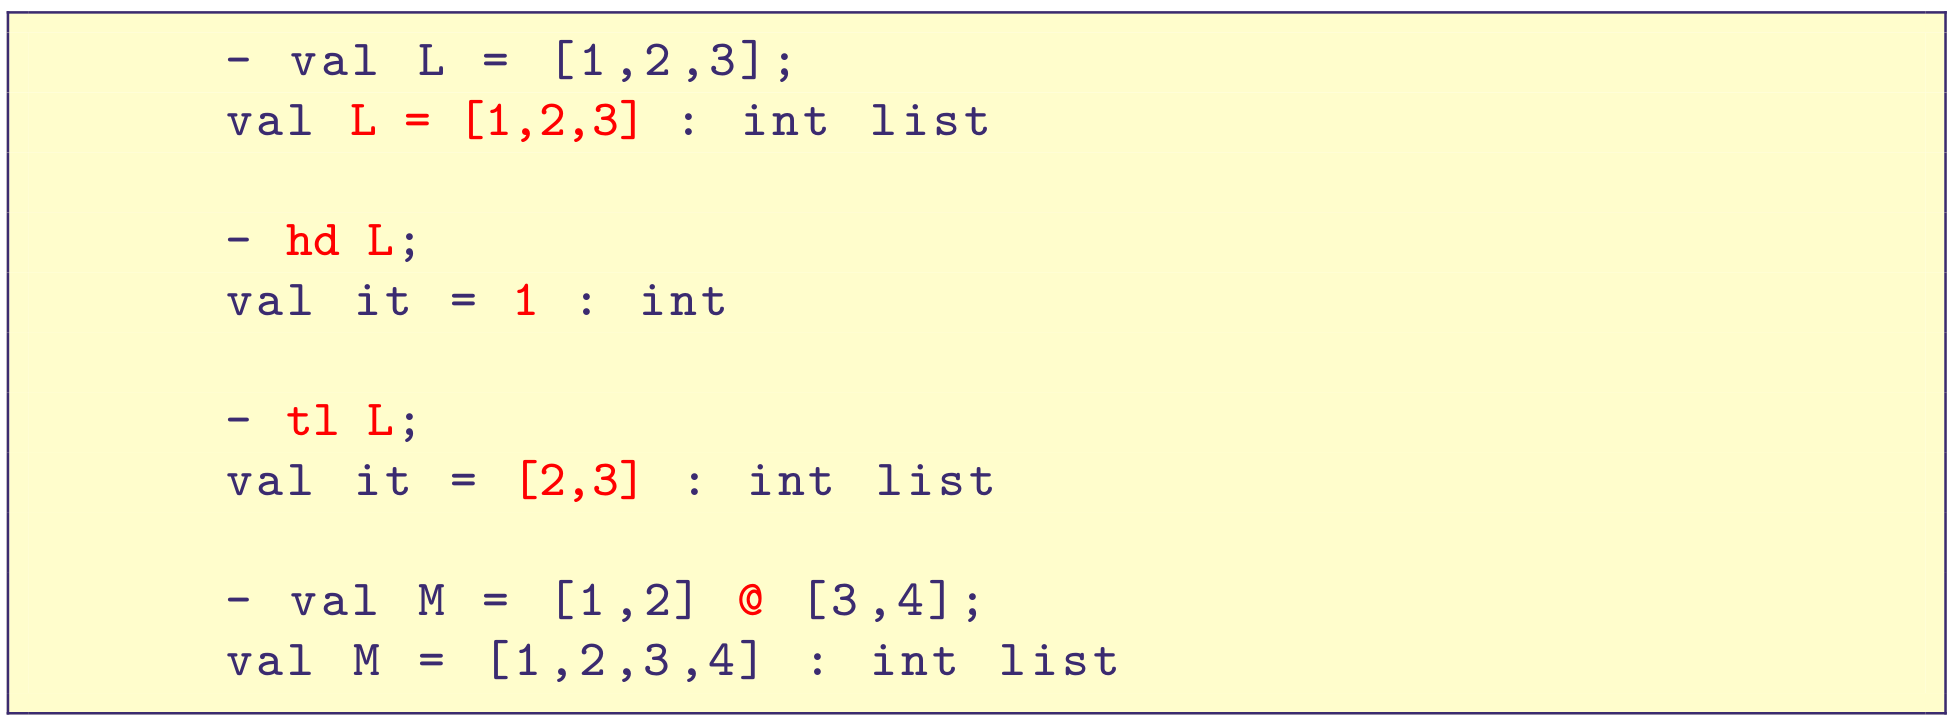
\includegraphics[scale=0.2]{Immagini/ml26.png}
\subsubsection{Funzioni aggiuntive su liste}
Altre funzioni si trovano nella struttura List, ad esempio
\begin{itemize}
    \item List.nth(L,i) restituisce l’i-esimo elemento di L (partendo
da 0)
\item List.last(L) restituisce l’ultimo elemento di L
\end{itemize}
\subsection{Currying}
In realtà in ML ogni funzione ha un solo argomento.

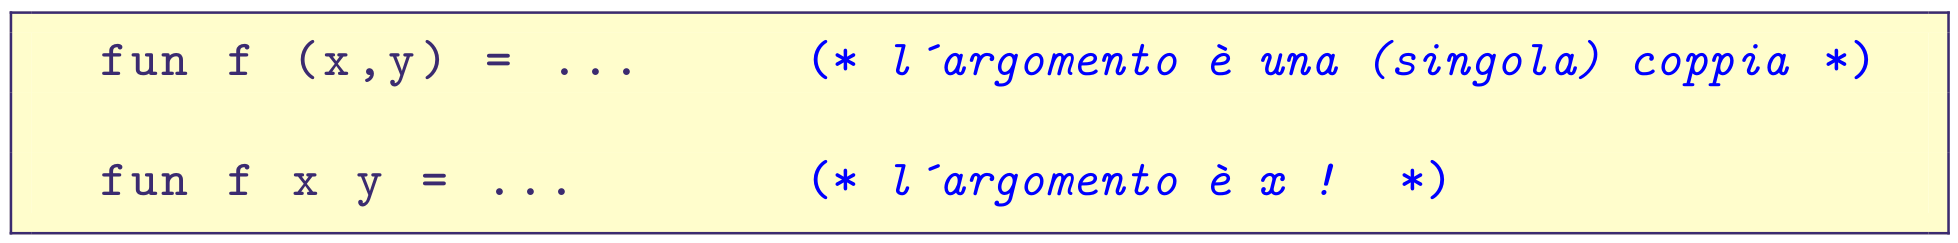
\includegraphics[scale=0.2]{Immagini/ml27.png}
\\Nel secondo caso, f è una funzione che restituisce una funzione
che prende y e calcola l’espressione dopo ‘=’.

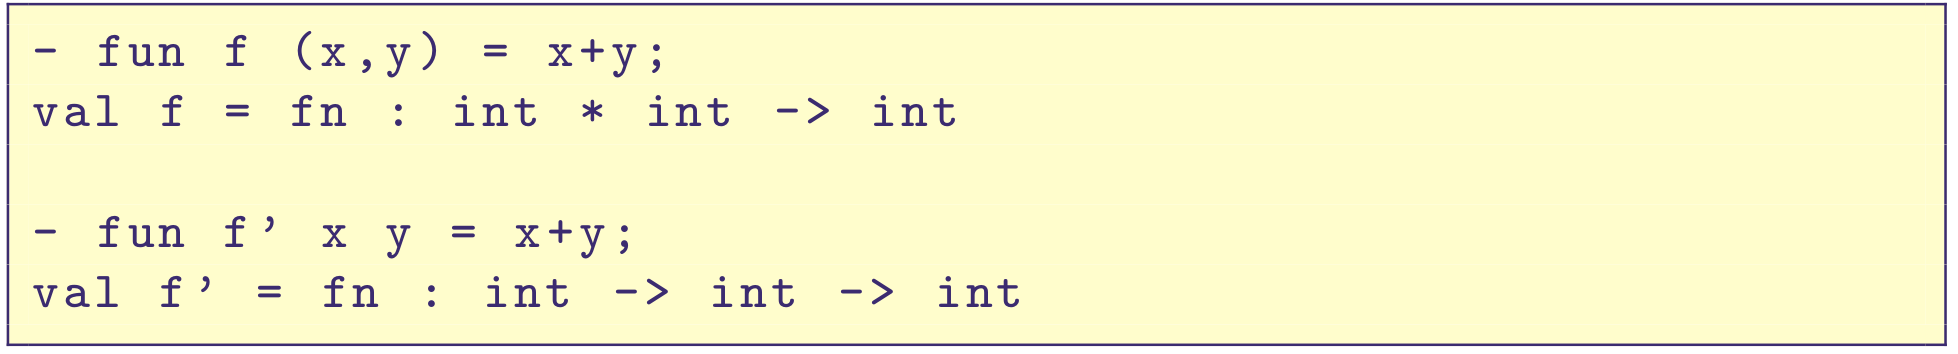
\includegraphics[scale=0.2]{Immagini/ml28.png}
Il tipo int $->$ int $->$ int va inteso come int $->$ (int $->$ int).

La trasformazione da n-uple (come f(x,y)) a funzioni che restituiscono
funzioni (come f’ x y) si chiama currying (dal nome di Haskell Curry).

L’utilizzo è ovviamente diverso.

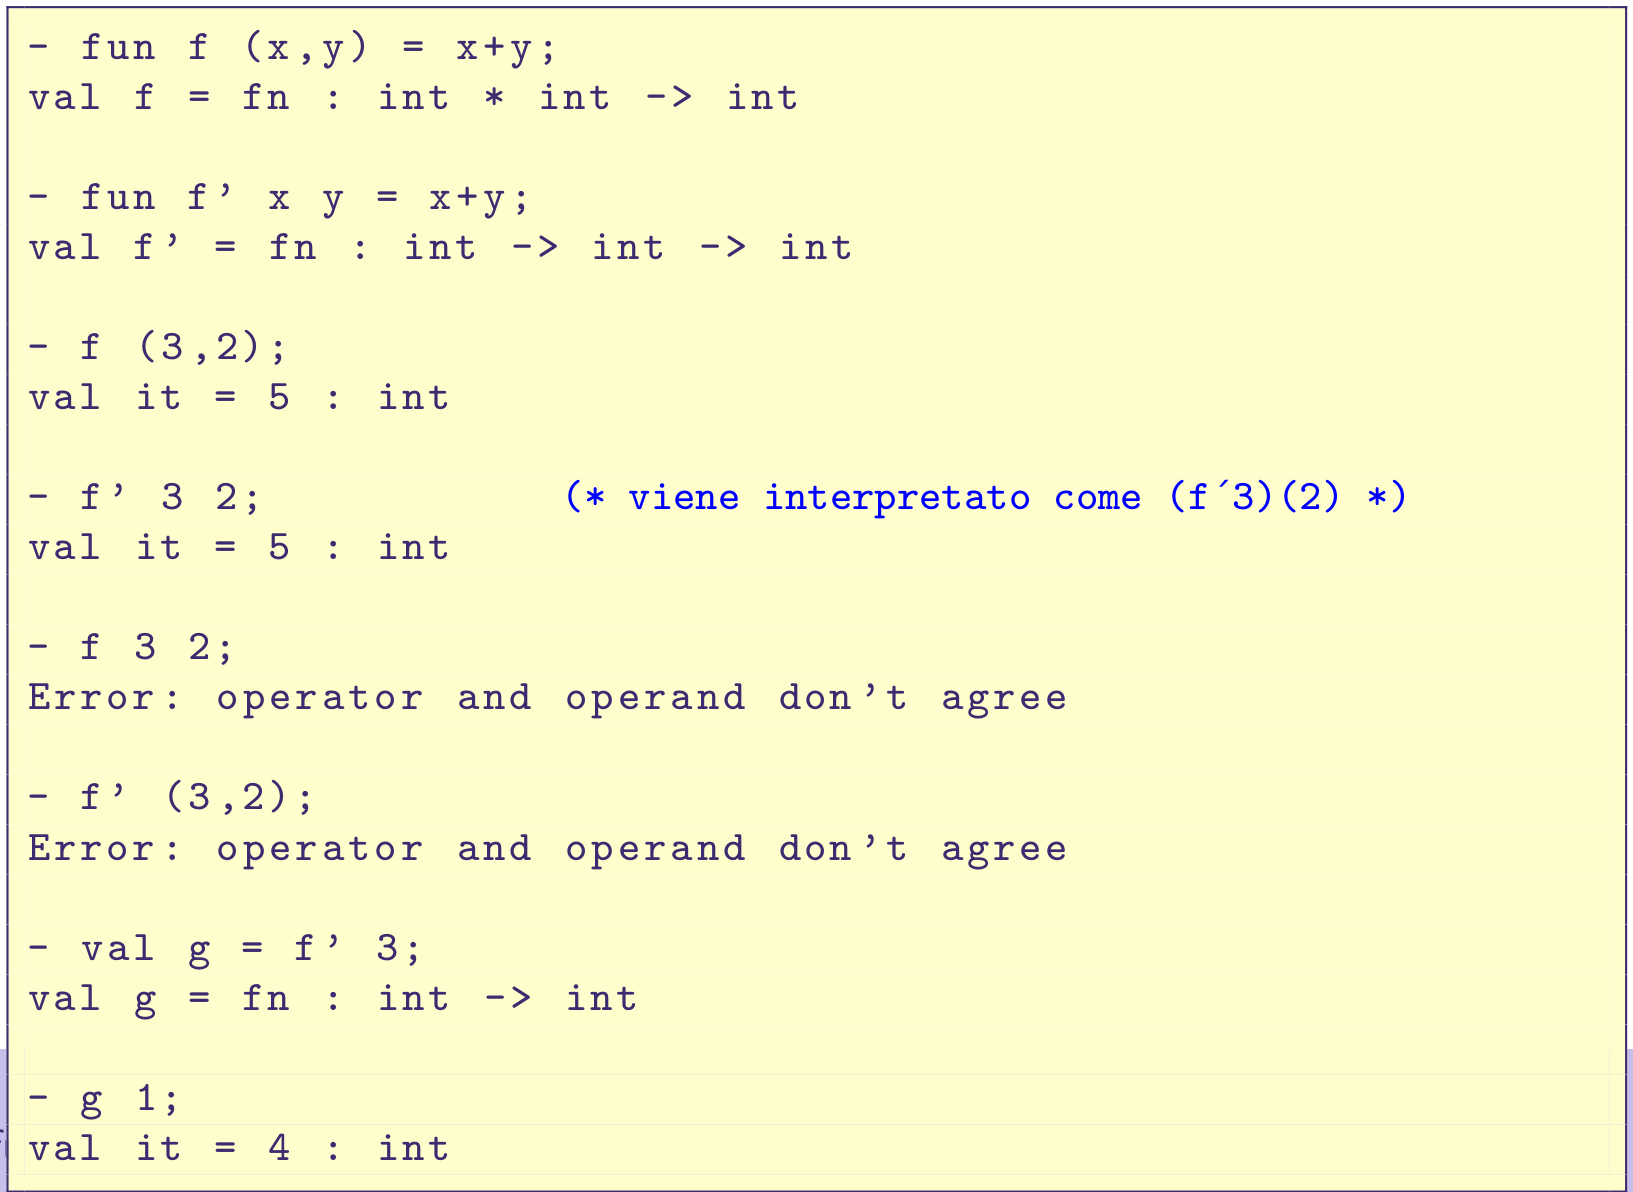
\includegraphics[scale=0.2]{Immagini/ml29.png}
\subsection{Funzioni di ordine superiore}
La maggior parte delle funzioni ricorsive che operano su liste,
alberi e simili hanno la stessa struttura; cambia solo l’operazione che si applica ai nodi.
Quindi basta scrivere una volta per tutte la funzione che
scandisce la struttura dati (che fa la funzione del ciclo)
e passargli la funzione da applicare ai nodi.
Le funzioni che hanno altre funzioni come parametri sono
dette di ordine superiore.

Una funzione f che esegue due volte una funzione g su un valore x:

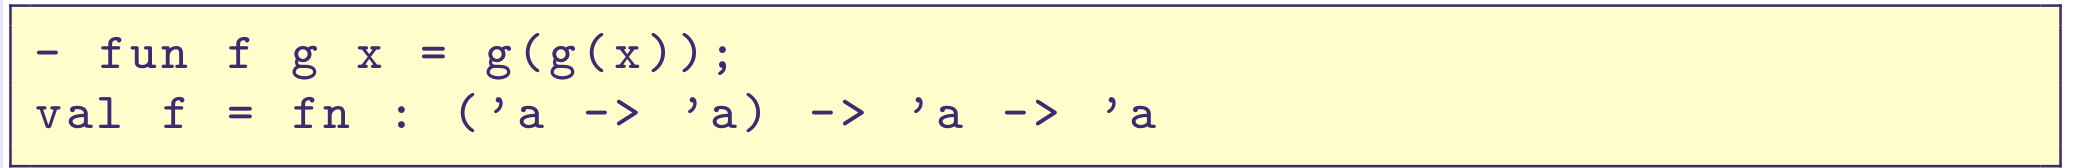
\includegraphics[scale=0.2]{Immagini/ml30.png}
\\\\
Equivalente in C (solo per interi):

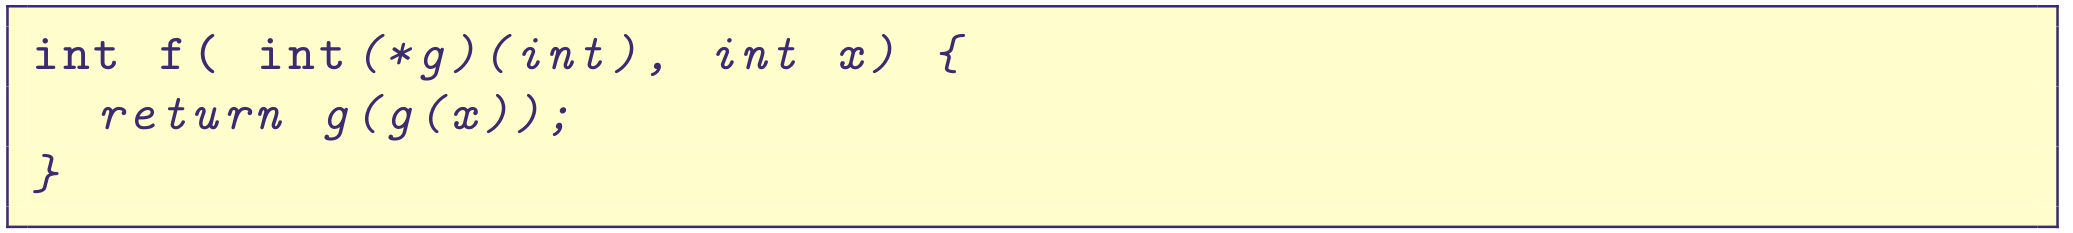
\includegraphics[scale=0.2]{Immagini/ml31.png}
Le tipologie di funzioni/ciclo più comuni sono tre:
\begin{itemize}
    \item filter
    \item map
    \item reduce/fold
\end{itemize}
\subsubsection{Filter}
La funzione filter prende una funzione booleana f e una lista L, seleziona gli elementi di L per cui f è vera.

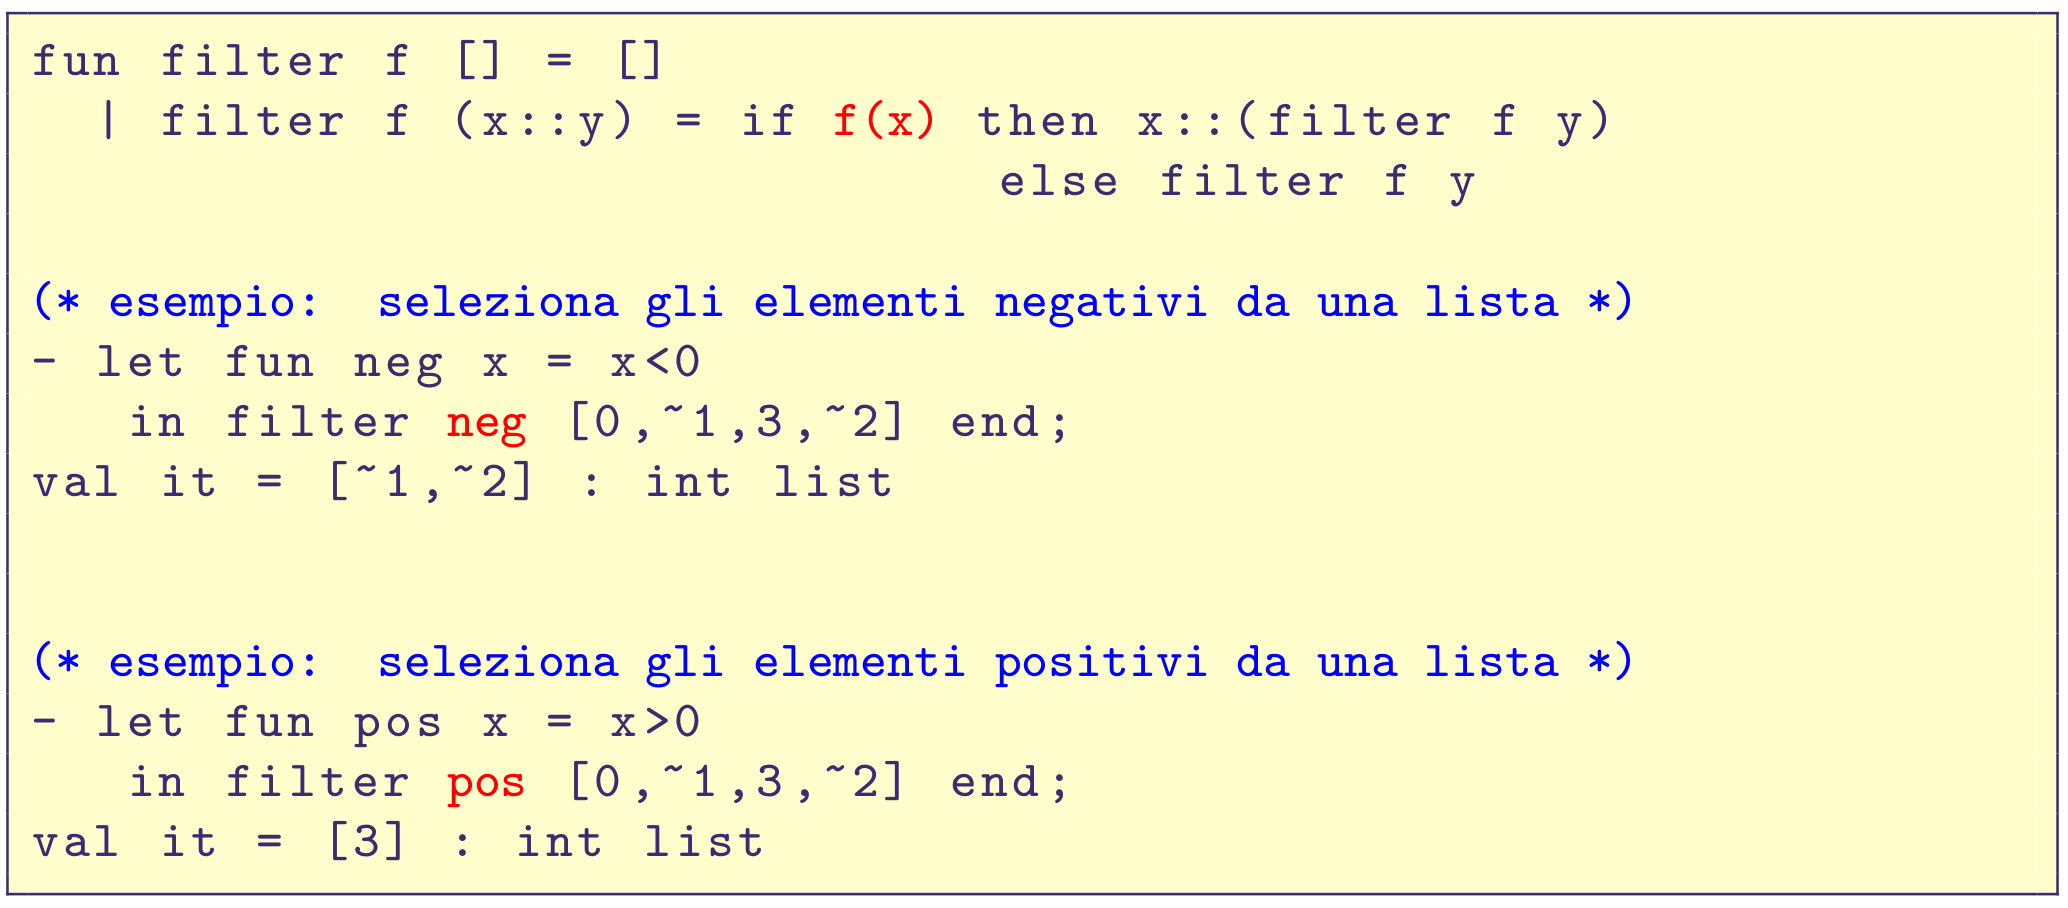
\includegraphics[scale=0.2]{Immagini/ml32.png}
\\\\
Nella libreria standard: List.filter
\subsubsection{Map}
La funzione map prende una funzione f e una lista L
applica f a tutti gli elementi della lista, ottenendo una nuova lista

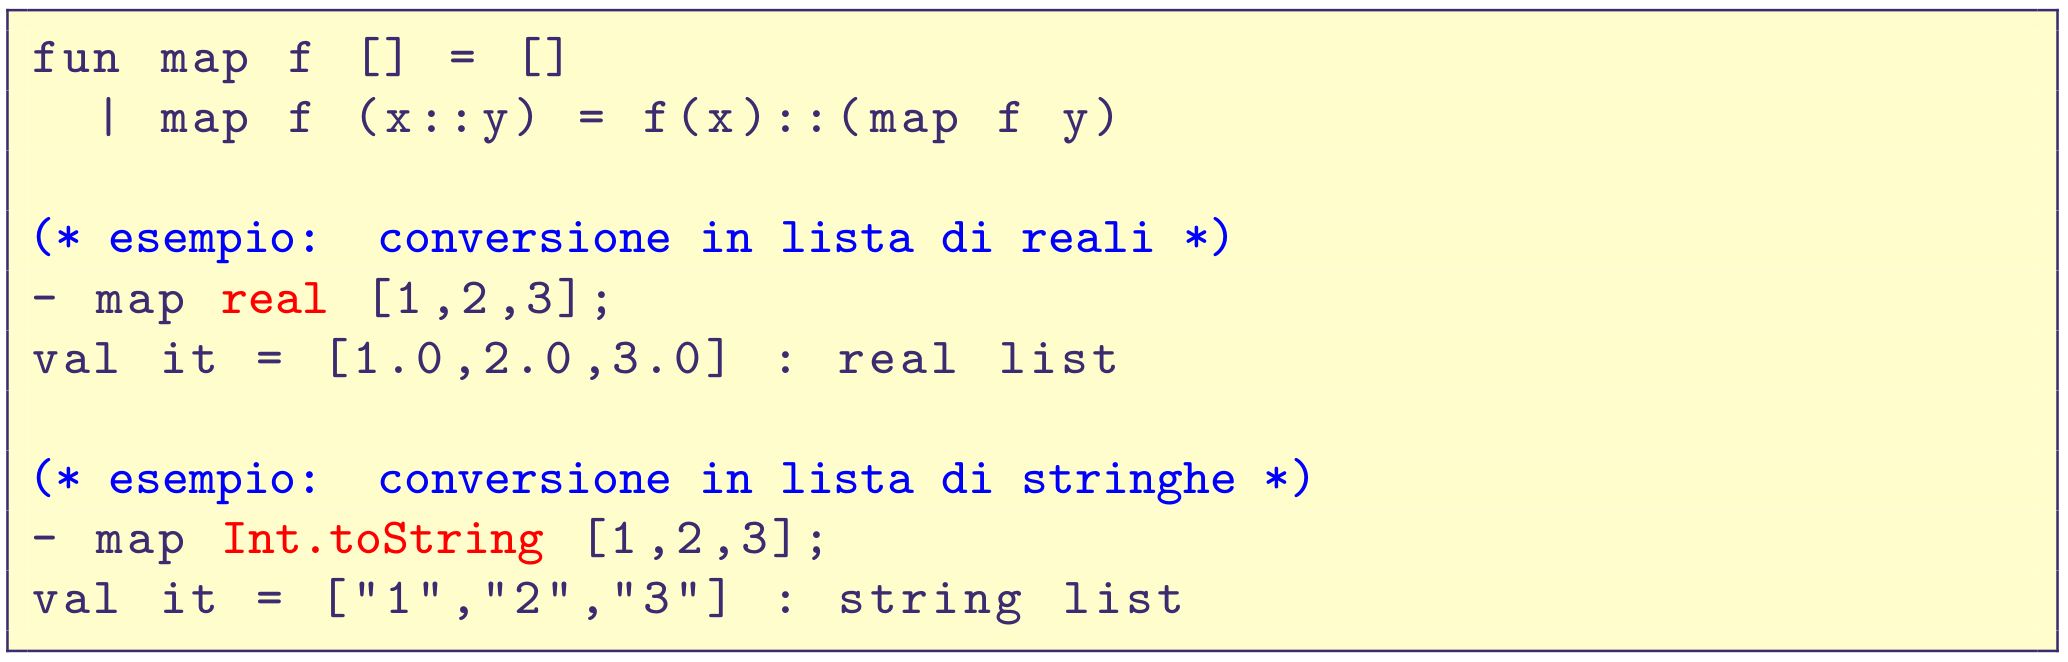
\includegraphics[scale=0.2]{Immagini/ml33.png}
\\\\
Nella libreria standard: List.map
\subsubsection{Reduce/fold}
La funzione reduce serve per calcolare aggregati di una lista

min, max, somma, prodotto, media...
\\\\
Prende in input una funzione a 2 argomenti f, un valore finale e
e una lista L ed effettua questo calcolo:

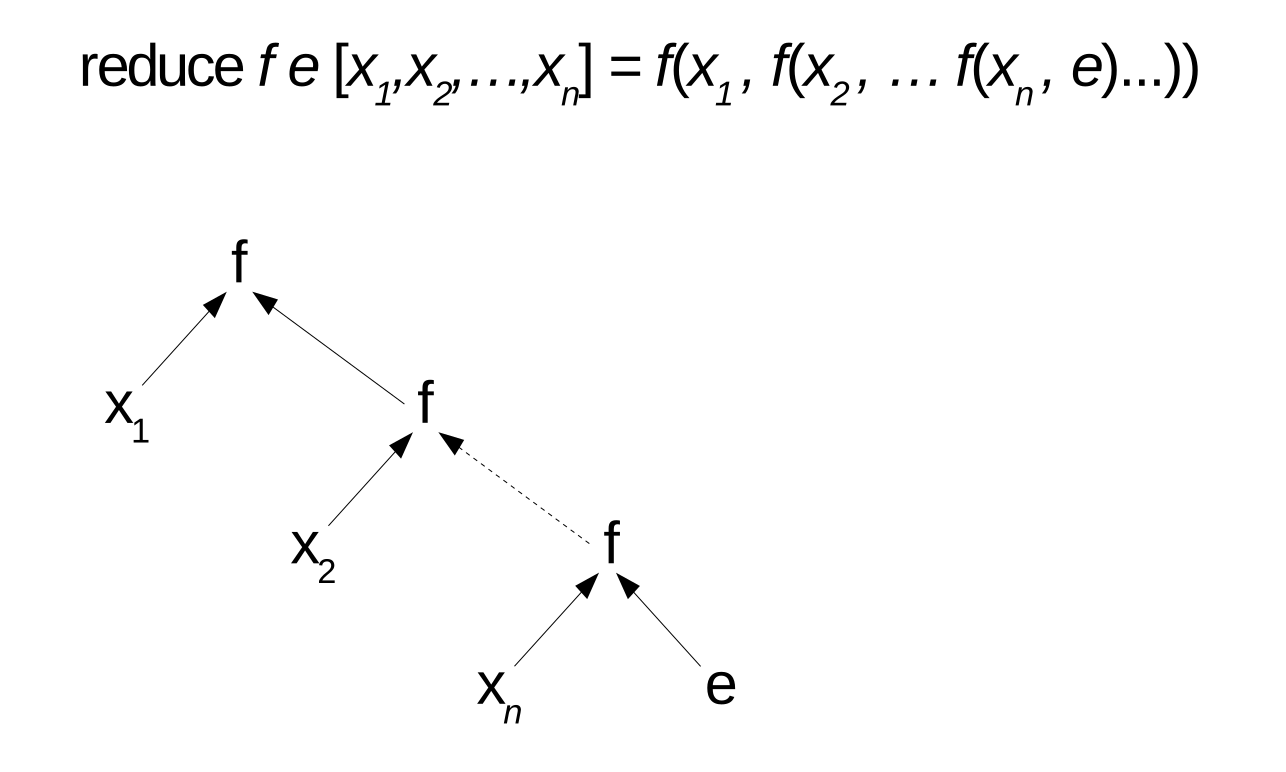
\includegraphics[scale=0.2]{Immagini/ml34.png}
\\\\
Ad esempio se f è ‘+’ ed e=0 allora reduce calcola la somma
degli elementi della lista.

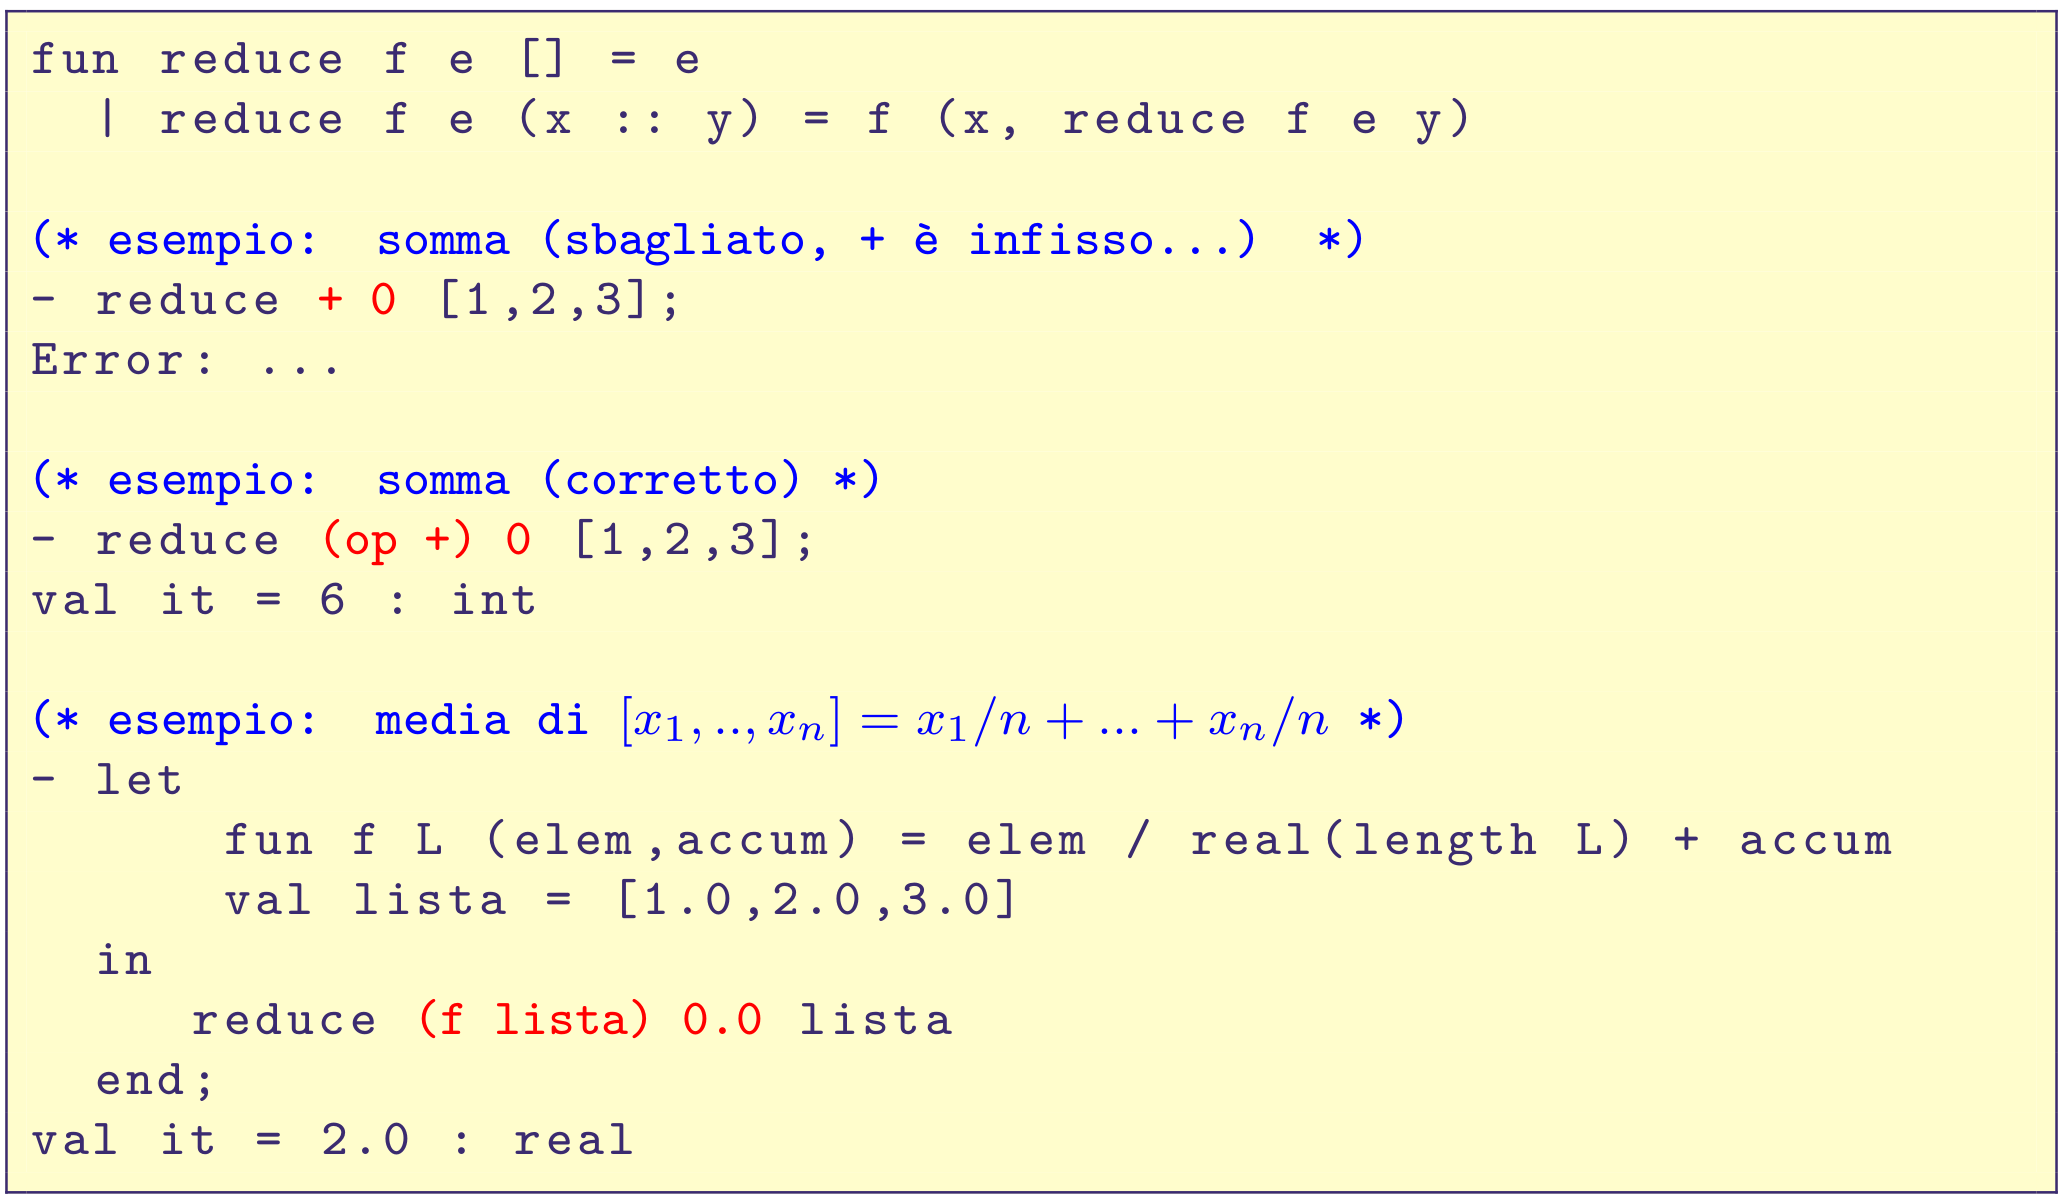
\includegraphics[scale=0.2]{Immagini/ml35.png}
\\\\
Simile alla funzione standard List.foldr

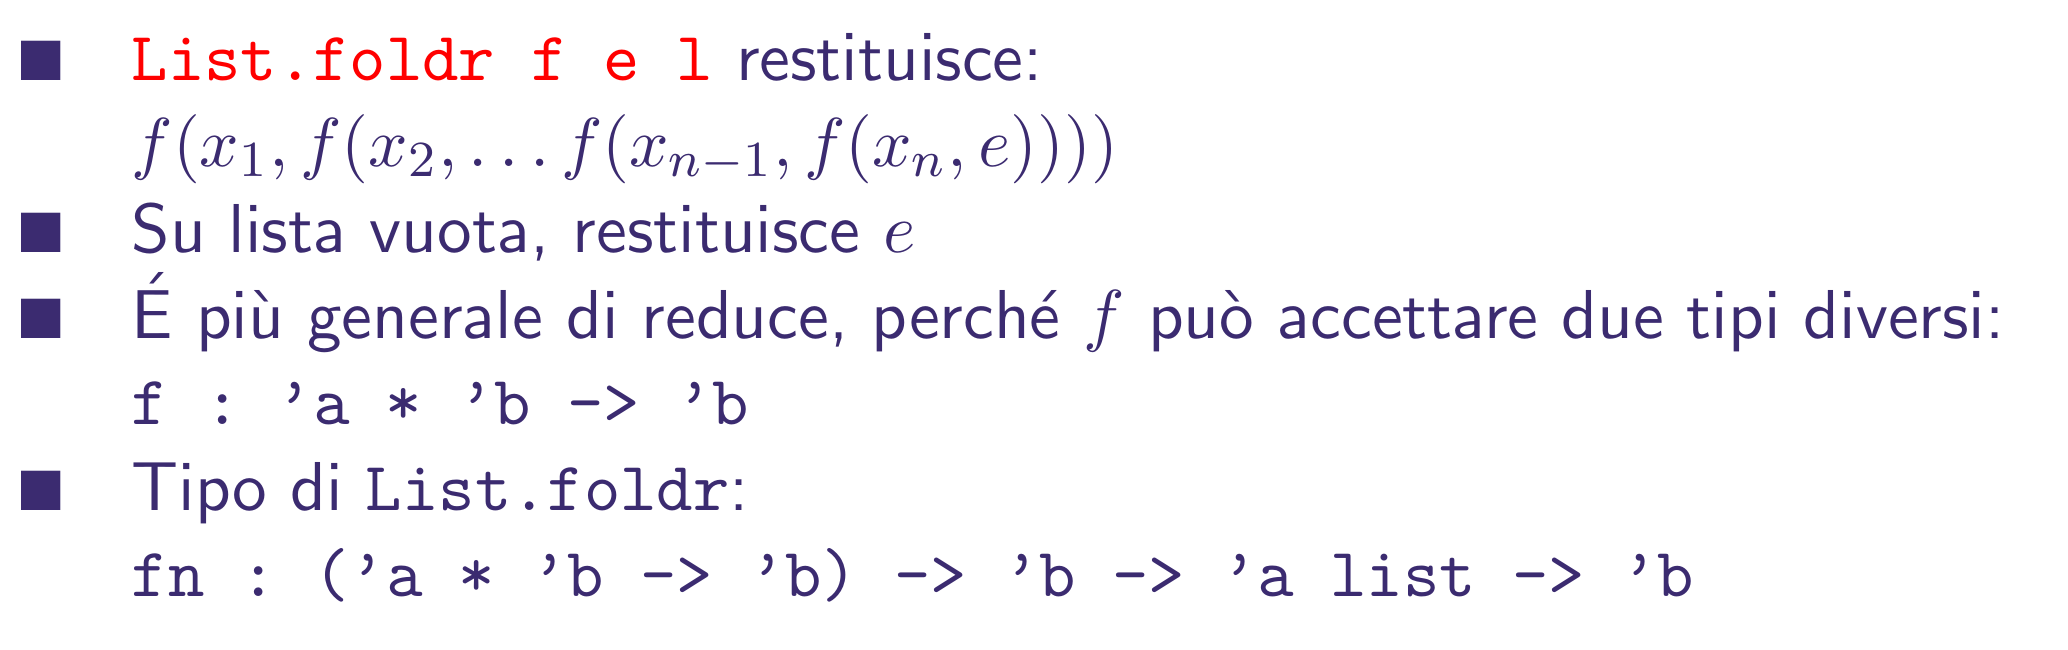
\includegraphics[scale=0.2]{Immagini/ml36.png}
\subsection{Funzioni anonime}
Quando utilizziamo funzioni di ordine superiori come filter, map e
reduce, può far comodo passargli funzioni semplici, specificate lì
per lì senza dover dare loro un nome (né usare un blocco let).

Queste funzioni anonime si specificano con la keyword \textbf{fn}

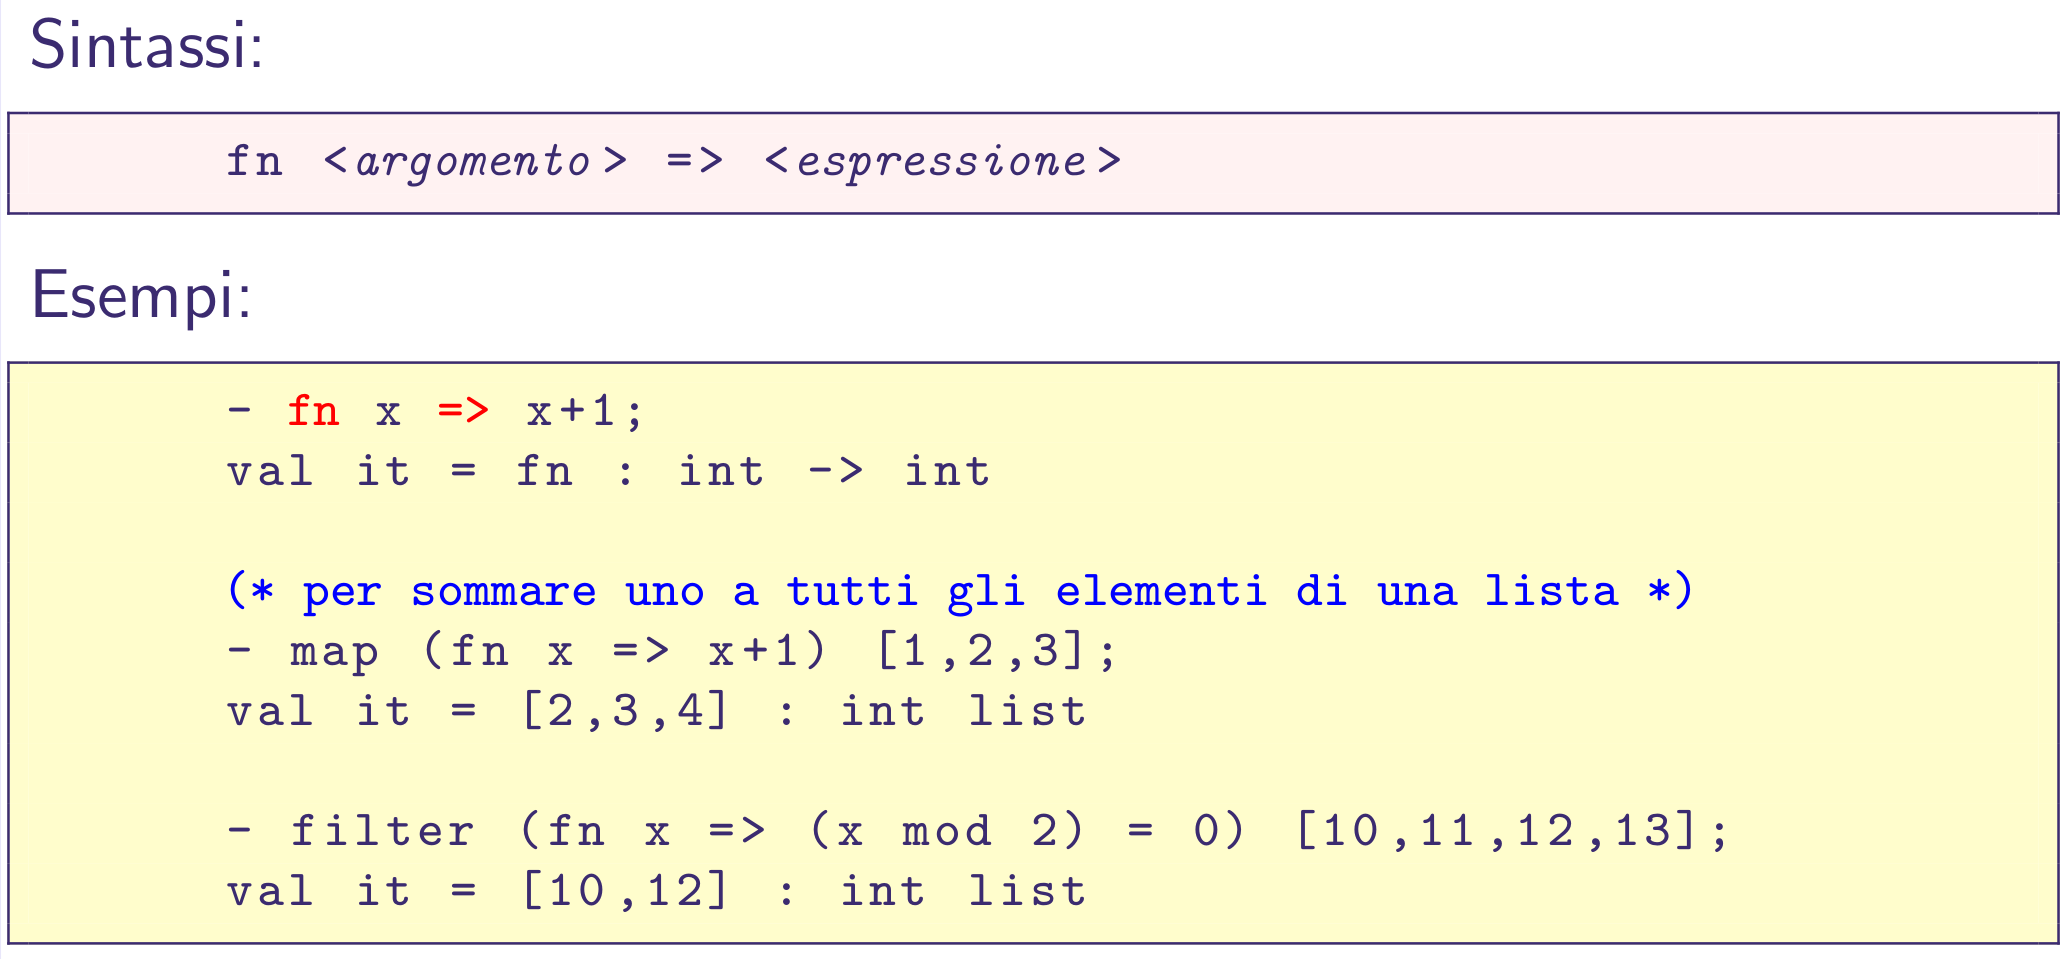
\includegraphics[scale=0.2]{Immagini/ml37.png}
\subsection{Val vs. fun}
Adesso possiamo vedere in che senso val è più generale di fun. Le
seguenti definizioni sono equivalenti:


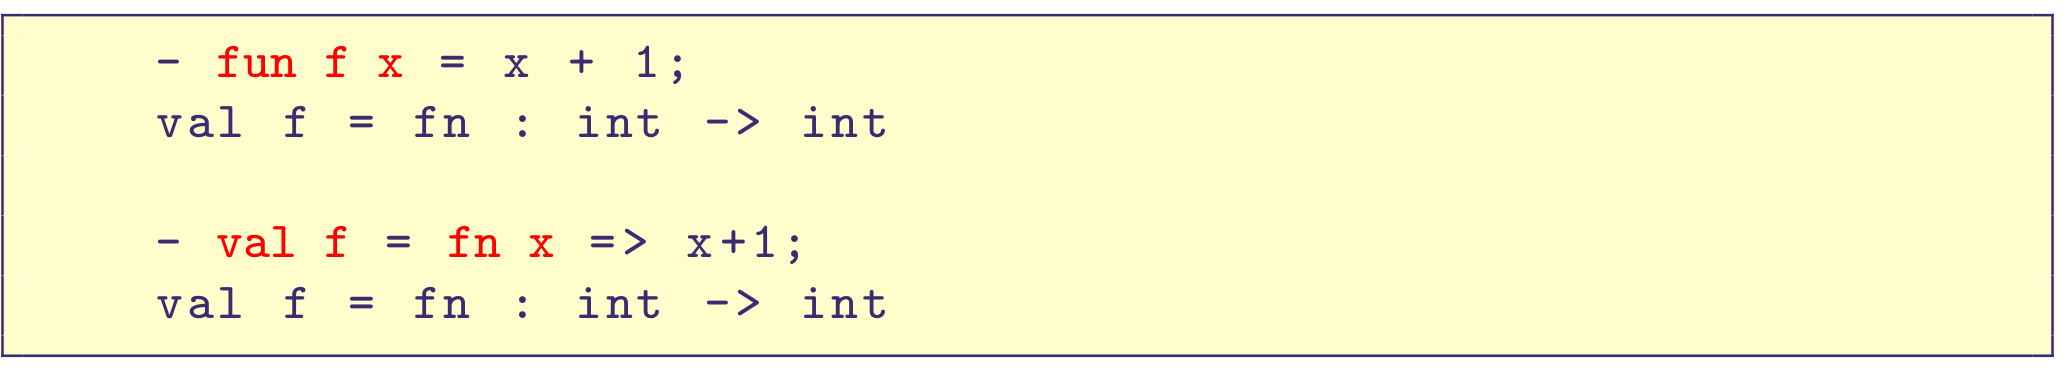
\includegraphics[scale=0.2]{Immagini/ml38.png}
\\
In altre parole, fun è zucchero sintattico, cioè una utile abbreviazione
per qualcosa che si potrebbe fare in altro modo (con val)
\subsection{Ulteriori dettagli su currying}
Adesso possiamo mostrare più esplicitamente la natura del
currying. Riprendiamo l’esempio:

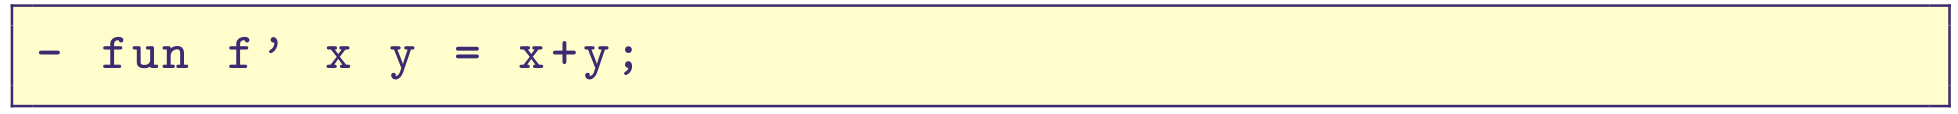
\includegraphics[scale=0.2]{Immagini/ml39.png}
\\\\
In effetti f’ può essere definita equivalentemente come

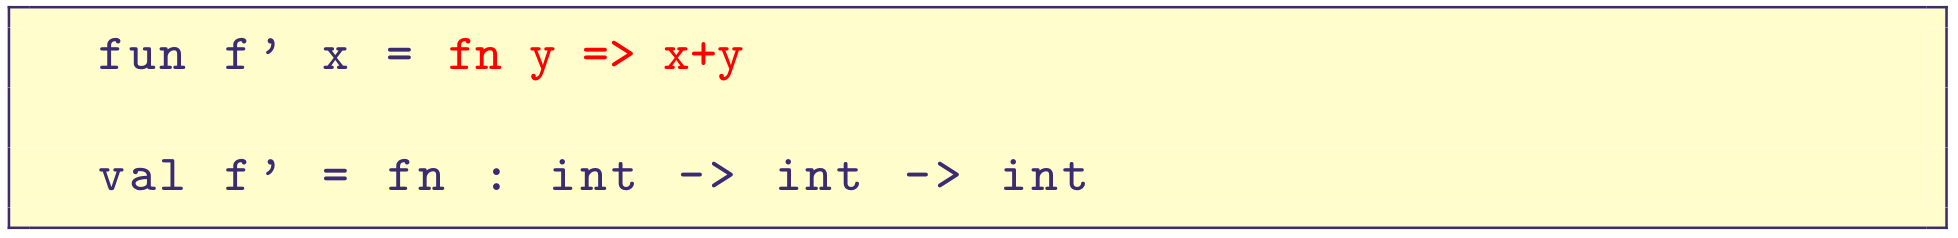
\includegraphics[scale=0.2]{Immagini/ml40.png}
\\\\
L’esempio della chiamata di f’ con un solo parametro può essere
spiegata così:

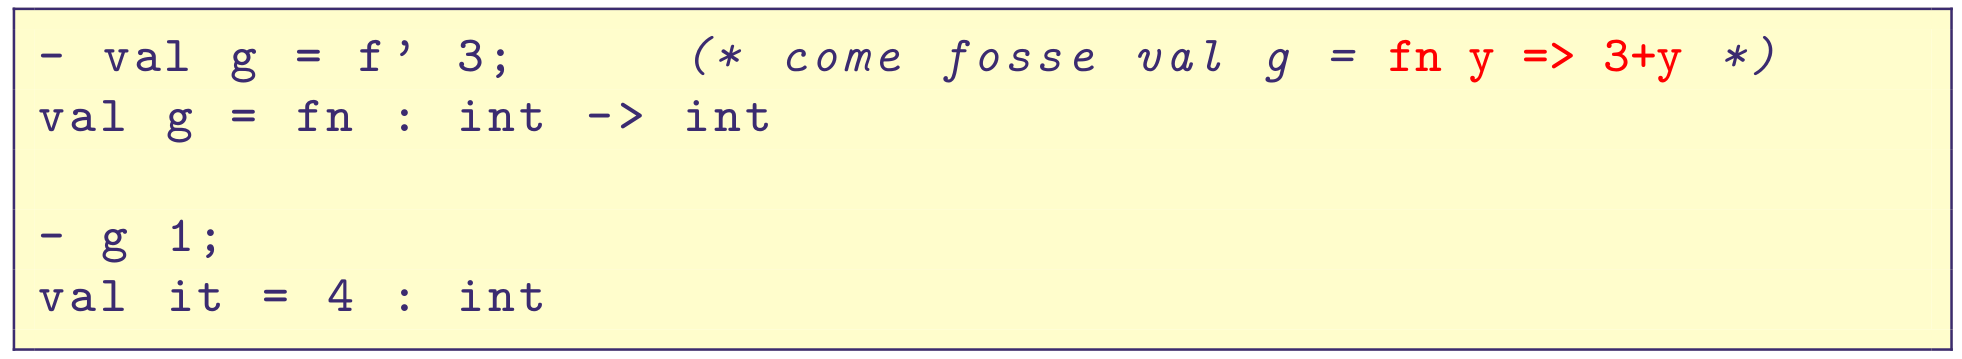
\includegraphics[scale=0.2]{Immagini/ml41.png}
\\\\
È anche possibile definire funzioni che effettuano il currying:


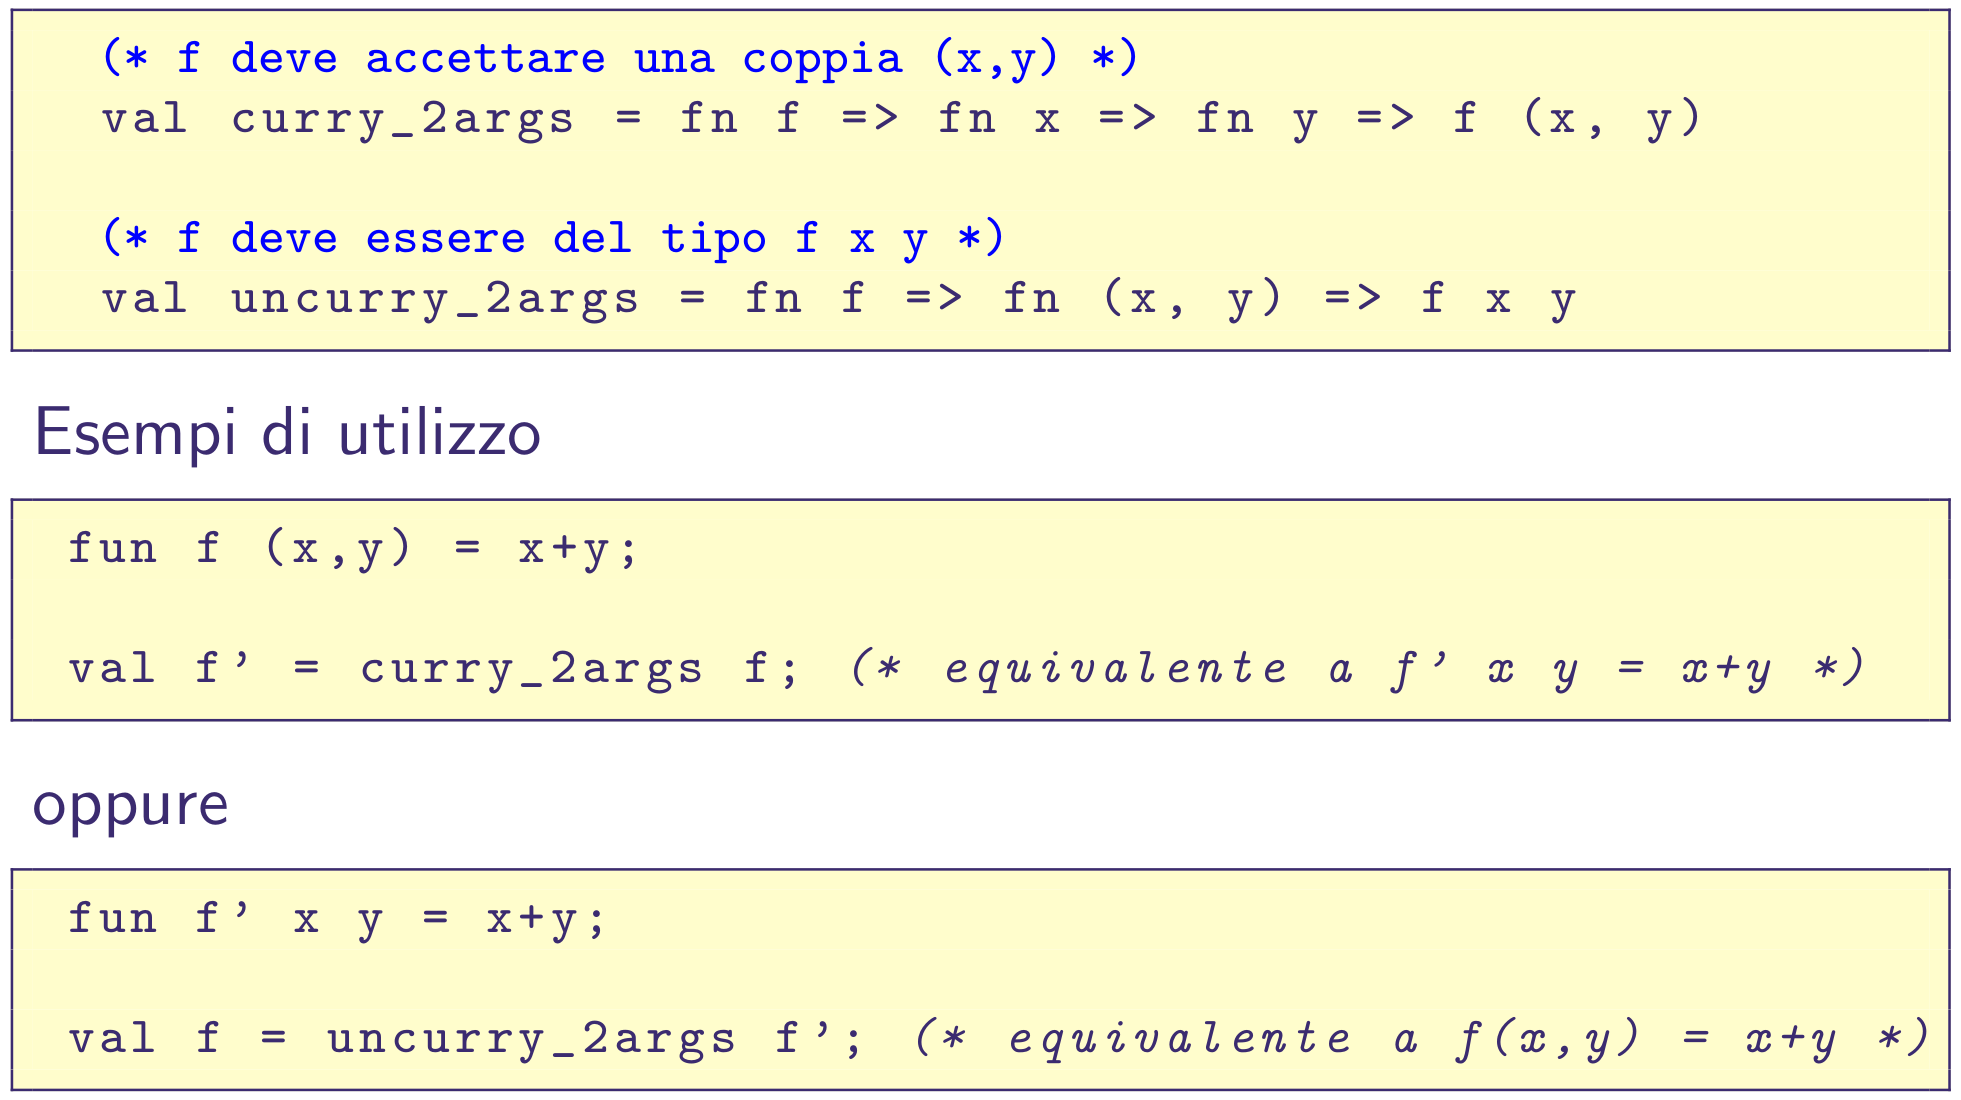
\includegraphics[scale=0.2]{Immagini/ml42.png}
\subsection{Polimorfismo parametrico}
Come definire tipi parametrici (come le liste)

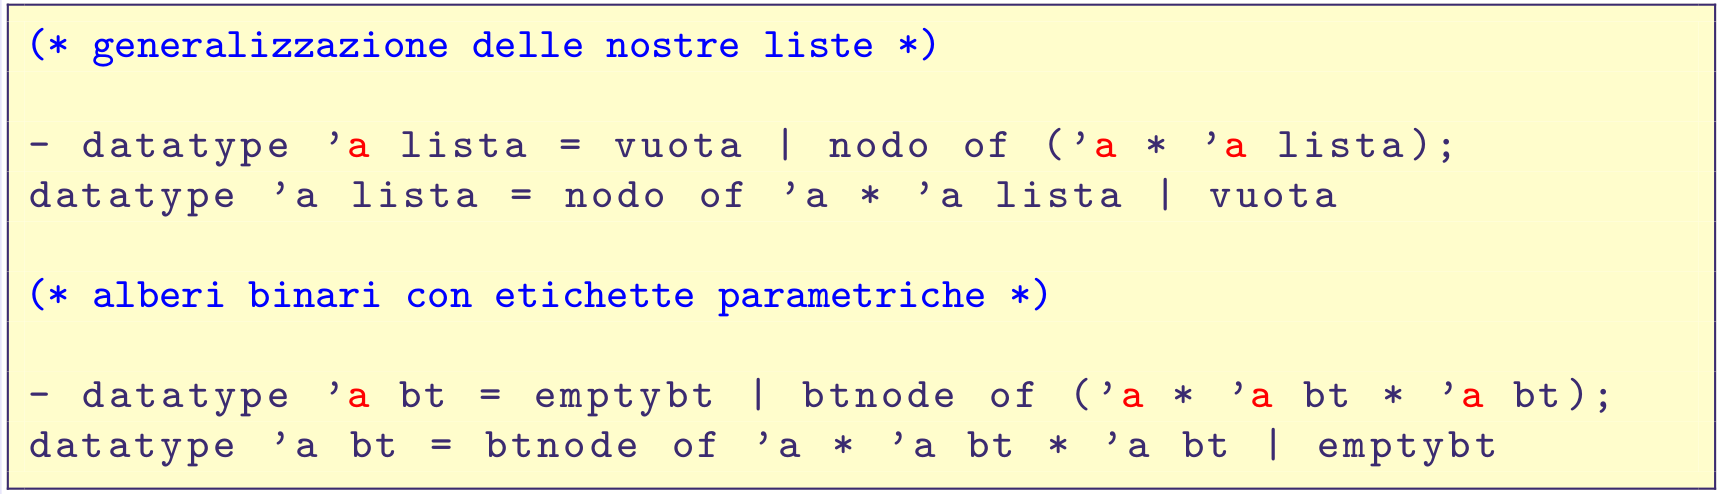
\includegraphics[scale=0.2]{Immagini/ml43.png}
\\\\
Per le funzioni (quando il compilatore non ha bisogno di aiuto
per stabilirne il tipo) non dobbiamo fare niente di speciale.
Ci pensa la \textbf{type inference}

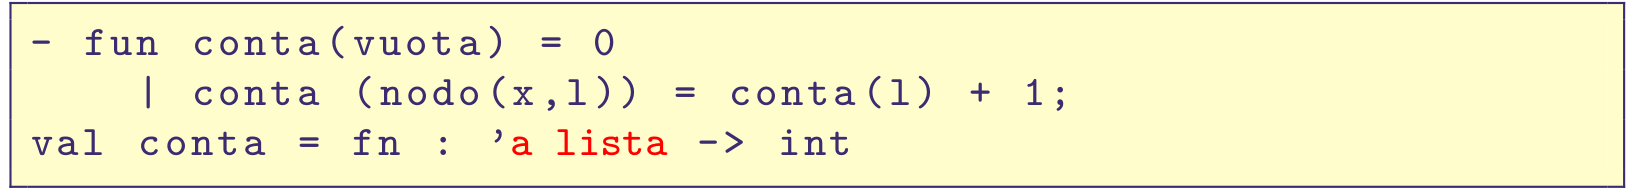
\includegraphics[scale=0.2]{Immagini/ml44.png}
\\\\
Come si può vedere dagli esempi precedenti ML usa l’apice prima
del nome per indicare che quella è una variabile di tipo

ad esempio ’a o ’b o ’c ...
\\
Quando si vuole che il tipo supporti l’uguaglianza, allora si mette
un doppio apice

ad esempio ”a o ”b o ”c ...
\\
Ogni tanto la type inference se ne accorge da sola

\includegraphics[scale=0.2]{Immagini/ml45.png}
\\
(ricordarsi che i reali non supportano l’uguaglianza...)
\subsection{Encapsulation e interfacce}
\subsubsection{Signatures}
Le signature sono il costrutto ML per definire interfacce (nel
senso di Java).
Definiscono tipi e funzioni senza specificare come sono
implementati.

\includegraphics[scale=0.2]{Immagini/ml46.png}
\\\\
\begin{itemize}
    \item dichiara un tipo parametrico ’a stack senza dire com’è definito
\item una funzione empty per costruire uno stack vuoto
\item una funzione push per inserire un elemento nello stack
\item una funzione pop per estrarre la testa dallo stack
\item ...senza dire come sono implementate (ovviamente)...
\item per assegnare un tipo a una espressione usare :
\end{itemize}
\subsubsection{Structures}
Le structure, come le classi, definiscono tipi di dato astratti.
Esempio di implementazione di STACK mediante una lista.

\includegraphics[scale=0.2]{Immagini/ml47.png}

Con l’espressione Stack :> STACK diciamo diverse cose:
\begin{enumerate}
    \item Stack deve implementare tutti gli identificatori dichiarati in STACK
    \item I tipi di dato dichiarati in Stack possono essere utilizzati solo con le
operazioni dichiarate in STACK
\end{enumerate}
Ogni altra funzione definita nella structure non è accessibile da fuori, cosıì si ottiene l’encapsulation, e si definiscono tipi di dato astratti.
\subsection{Incapsulamento dell’implementazione dei tipi}
Anche se in Stack il tipo stack è implementato con list non si può usare come list perché la structure Stack non mette a disposizione alcuna
funzione length sul tipo stack e ne nasconde l’implementazione.

\includegraphics[scale=0.2]{Immagini/ml48.png}

\includegraphics[scale=0.2]{Immagini/ml49.png}
\subsection{Functors}
Alcune delle componenti di una structure possono essere variabili
ed essere specificate come dei parametri.
Si usa una keyword diversa: functor. Analogo dei template.
Ecco un esempio di definizione di immagini parametrica rispetto
alla codifica del colore.
Supponiamo di avere due structure RGB e CMYK per gli
omonimi modelli di colore e che entrambe implementino la signature COLOR.
La struttura parametrica si può dichiarare così:

\includegraphics[scale=0.2]{Immagini/ml50.png}
\subsection{Eccezioni}
Come Java, anche ML ha le sue eccezioni predefinite...

\includegraphics[scale=0.2]{Immagini/ml51.png}
\\\\
In ML la gestione delle eccezioni è integrata col type checking

\includegraphics[scale=0.2]{Immagini/ml52.png}
\\\\
Ecco come funziona:
\begin{enumerate}
    \item la type inference capisce che l’input di pop è una lista
    \item il datatype lista ha due costruttori: :: e [ ]
    \item la definizione per casi di pop ha un caso solo per ::
da cui il warning
\item il compilatore inserisce automaticamente una eccezione Match nei
casi mancanti
\end{enumerate}
\subsubsection{Dichiarazione e generazione eccezioni}
Il programmatore può definire le proprie eccezioni:

\includegraphics[scale=0.2]{Immagini/ml53.png}
\\\\
Il risultato in caso di errore è più esplicativo dell’eccezione
“automatica” Match

\includegraphics[scale=0.2]{Immagini/ml54.png}
\\\\
Le eccezioni possono essere catturate e gestite con handle:

\includegraphics[scale=0.2]{Immagini/ml55.png}
\\\\
Il costrutto handle può essere messo dopo qualunque espressione che può generare
una eccezione.
Un singolo handle può gestire diverse eccezioni.

\includegraphics[scale=0.2]{Immagini/ml56.png}
\\\\
Due modi di usarlo in ML funzionale puro:
\begin{enumerate}
    \item fare qualcosa come stampare un messaggio e rilanciare l’eccezione
    \item “aggiustare” l’errore restituendo un valore dello stesso tipo
dell’espressione che ha sollevato l’eccezione
\end{enumerate}
Sono le uniche opzioni che passano il type checking senza errori
\subsubsection{Eccezioni con parametri}
Si possono aggiungere dettagli sull’errore che si è verificato
aggiungendo parametri alle eccezioni

\includegraphics[scale=0.2]{Immagini/ml57.png}
\\\\
\section{Compilatore di espressioni in ML}
ML – come gli altri linguaggi dichiarativi (= non imperativi) – è
particolarmente adatto alla manipolazione di simboli.

La realizzazione di compilatori è un esempio di questo tipo di
problema dove bisogna elaborare espressioni e comandi di un linguaggio di
programmazione (codice sorgente) e tradurli in un altro
linguaggio (codice oggetto o intermedio).

\subsection{Procedimento di valutazione delle espressioni}
\includegraphics[scale=0.2]{Immagini/comp1.png}
\subsection{Definizione degli alberi sintattici}
Introduciamo un costruttore per ogni operazione supportata dal
linguaggio sorgente dove 
ogni costruttore corrisponde a un tipo di nodo dell’albero
sintattico.

\includegraphics[scale=0.3]{Immagini/comp2.png}
\subsection{Definizione del linguaggio target}
Le operazioni della macchina astratta che eseguirà il
codice oggetto sorgente (prendono ispirazione dalle istruzioni di un hardware classico).

\includegraphics[scale=0.3]{Immagini/comp3.png}
\\\\
Obiettivo: terminare il programma con il risultato in cima allo stack.
\subsection{Generazione del codice – funzione codegen}
Il codice oggetto utilizza tre registri:
\begin{itemize}
    \item R1 come puntatore alla testa dello stack
    \item R2 ed R3 per calcolare le singole operazioni
\end{itemize}
La traduzione vera e propria è effettuata da una funzione ausiliaria translate che prende in input:
\begin{itemize}
    \item un albero sintattico \textbf{tree}
    \item una \textbf{continuazione}, ovvero il codice da eseguire dopo aver eseguito le operazioni
    contenute in \textbf{tree}
\end{itemize}
Pertanto alla prima chiamata di translate verranno passati
\begin{itemize}
    \item l’albero sintattico dell’intera espressione da compilare
    \item la lista di istruzioni [HALT]
\end{itemize}
\subsection{Ottimizzazione del codice - funzione optimize}
La generazione automatica introduce operazioni inutili.

\includegraphics[scale=0.3]{Immagini/comp4.png}
\\\\
La funzione optimize elimina le più comuni operazioni
ridondanti.
Itera una funzione ausiliaria opt1 che esegue un singolo passo di
ottimizzazione.
Questo può attivare ulteriori semplificazioni, quindi optimize
itera opt1 finchè il codice non può essere ulteriormente ridotto.

\includegraphics[scale=0.3]{Immagini/comp5.png}
\\\\
Ecco il risultato per la solita espressione 3+5*2. A sinistra il
codice non ottimizzato, a destra quello ottimizzato.

\includegraphics[scale=0.3]{Immagini/comp6.png}
\subsection{Combinare le fasi con composizione di funzioni}
L’operatore \textbf{o} denota la composizione di funzioni

(f o g)(x) = f(g(x))
\\
Con la composizione è facile definire l’intero processo di
compilazione assemblando le diverse fasi.

\includegraphics[scale=0.3]{Immagini/comp7.png}
\subsection{Conclusioni}
La combinazione di costruttori, pattern e definizione per casi
rende le trasformazioni del codice sorgente e del codice oggetto
particolarmente chiare. 

In Java, che pure è un ottimo linguaggio, ogni nodo
dell’albero sintattico sarebbe un oggetto e “leggere” la
struttura di pezzi di albero non sarebbe immediato.

Inoltre la type inference ci permette di omettere il tipo degli
identificatori, producendo un codice più snello come fosse uno scripting language debolmente tipato,v ma senza sacrificare il controllo di tipi forte.

Per queste ragioni linguaggi come ML vengono utilizzati per la
prototipizzazione rapida di compilatori e interpreti.

\section{Paradigma Logico - Prolog}
\textbf{Programmi} = insiemi di assiomi.
\\
\textbf{Computazioni} = dimostrazioni costruttive di una formula logica
data – detta \textit{query} – mediante gli assiomi del programma.
\\
\textbf{Esempio}
\begin{itemize}
    \item Programma
    \begin{itemize}
        \item Socrate è un uomo. (assioma 1)
        \item Tutti gli uomini sono mortali. (assioma 2)
    \end{itemize}
    \item Query 1
    \begin{itemize}
        \item Socrate è un uomo?
        \item riposta: yes
    \end{itemize}
    \item Query 2
    \begin{itemize}
        \item Socrate è mortale?
        \item riposta: yes
    \end{itemize}
\end{itemize}
\subsection{Implementazione e Interazione in Prolog}
L’implementazione è mista: I programmi Prolog vengono compilati in un bytecode
che viene interpretato da una macchina virtuale,
la Warren abstract machine (WAM),
si possono anche compilare i programmi in codice
stand-alone, direttamente eseguibile.

L’interazione con Prolog è analoga a quella con ML, si inviano query all’interprete e si ottengono le relative risposte
oppure, se il programma è stand alone, si interagisce
mediante la sua UI (user interface).

SWI Prolog (free) implementa il Prolog standard,
supporta sia interpretazione che compilazione stand-alone.
Invocazione da command line:

\includegraphics[scale=0.2]{Immagini/prolog1.png}
\subsection{Costrutti base}
Tre tipi di statement:
\begin{enumerate}
    \item facts
    \item rules
    \item queries (dette anche goals)
\end{enumerate}
Una sola struttura dati:
\begin{enumerate}
    \item logical terms
\end{enumerate}
\subsection{Fatti}
Asseriscono una relazione tra oggetti

\includegraphics[scale=0.2]{Immagini/prolog2.png}

father, oltre che relazione, è chiamato anche predicato
\\
Altro esempio: le tabelline

\includegraphics[scale=0.2]{Immagini/prolog3.png}
\\
I nomi dei predicati devono iniziare per lettera minuscola.

Gli argomenti abraham e isaac iniziano con lettera minuscola
perchè sono costanti, come i numeri.

Con i fatti possiamo definire un database. Ogni predicato corrisponde a una tabella relazionale.
\subsection{Queries}
I programmi logici sono fatti per rispondere a queries.
Le query hanno la stessa forma dei fatti. Sono entrambi dei
cosiddetti atomi logici. nei programmi sono asserzioni (fatti) mentre
nelle query sono domande.
\subsection{Variabili logiche nelle query}
È utile chiedere cose come: quali sono i figli di abraham? 
Si può fare con le variabili logiche 
che si riconoscono perchè iniziano con una lettera maiuscola.

\includegraphics[scale=0.2]{Immagini/prolog4.png}
\\
La macchina virtuale cerca i valori che – sostituiti a X – rendono
la query uguale a uno dei fatti nel programma. 

NB: questo vale per i programmi di soli fatti...
\\
Differenza tra le variabili logiche e le variabili degli altri paradigmi
\begin{itemize}
    \item Le variabili logiche rappresentano oggetti qualsiasi, non specificati
    \item Le variabili dei linguaggi imperativi sono locazioni di memoria
    \item Gli identificatori dei linguaggi funzionali denotano valori immutabili
\end{itemize}
Si possono usare anche nei fatti. Un credente potrebbe scrivere
in un programma:

\includegraphics[scale=0.2]{Immagini/prolog5.png}
\\
Differenza tra le variabili nei fatti e nelle query:
\begin{itemize}
    \item nelle query: esistenzialmente quantificate
    \begin{itemize}
        \item esiste un X tale che ... ?
    \end{itemize}
    \item nei fatti: universalmente quantificate
    \begin{itemize}
        \item per ogni X vale che ...
    \end{itemize}
\end{itemize}
\subsection{I termini}
I termini sono l’unica struttura dati in Prolog. 
Si costruiscono con costanti, variabili (logiche) e funtori.
I funtori hanno un ruolo simile ai costruttori di ML, sono
caratterizzati da nome e arietà (il numero di argomenti)

\includegraphics[scale=0.2]{Immagini/prolog6.png}
\\
Non ci sono dichiarazioni di tipo.
Costanti simboliche e funtori si usano senza dichiararli prima.
\\
Gli argomenti di un predicato possono essere termini qualsiasi.

\includegraphics[scale=0.2]{Immagini/prolog7.png}
\\
Esempi di query a un programma coi fatti qui sopra

\includegraphics[scale=0.2]{Immagini/prolog8.png}
\\
La stessa variabile X può comparire più volte nello stesso fatto o
nella stessa query. Significa che i termini nelle posizioni dove si trova X devono
essere uguali tra loro.

\includegraphics[scale=0.2]{Immagini/prolog9.png}
\\
\subsubsection{Differenza tra termini di Prolog e pattern di ML}
In ML non posso usare la stessa variabile più volte nello
stesso pattern
perchè servono solo a estrarre informazioni da una struttura,
non a controllare se elementi diversi sono uguali.
\subsection{Ground e nonground}
Un termine è ground se non contiene variabili
Altrimenti è nonground

\includegraphics[scale=0.2]{Immagini/prolog10.png}
\\
Gli stessi aggettivi e gli stessi criteri si applicano ai fatti, alle
query e anche alle regole.

\includegraphics[scale=0.2]{Immagini/prolog11.png}
\subsection{Come si risponde alle query}
Per spiegarlo dobbiamo specificare come avviene il matching tra
query e fatti e come si costruiscono le risposte
Dovremo introdurre due nozioni:
\begin{itemize}
    \item sostituzione
    \item unificazione
\end{itemize}
\subsubsection{Sostituzioni}
Una sostituzione è un insieme finito di coppie:

$\theta = \{X1 = t1 , . . . Xn = tn \}$
\\
dove
\begin{itemize}
    \item Le $X_i$ sono variabili e i $t_i$ termini.
    \item Le $X_i$ sono tutte diverse tra loro.
    \item Nessuna delle $X_i$ compare dentro i $t_i$ .
\end{itemize}
L’applicazione di $\theta$ a una espressione $E$ (che potrebbe essere un
termine, un fatto, una query o una regola) si denota con $E\theta$.
Sostituisce le occorrenze delle variabili $X_i$ in $E$ con i rispettivi
termini $t_i$.
\\
Esempio:

se $\theta$ = $\{X = isaac\}$ ed $E = father(abraham, X)$ 

allora $E\theta = father(abraham, isaac)$.

\subsubsection{Istanze}
L’applicazione di una sostituzione $\theta$ ad $E$ crea un “caso particolare” di $E$,
dove le variabili di $E$ (che indicano oggetti non specificati)
vengono sostituite con valori specifici (termini ground)
o parzialmente specificati (termini nonground).
\\
Esempio: 

$\theta = \{X = color(rgb, Y, Y, Y)\}$ ed $E = hasColor(o1, X).$

\begin{itemize}
    \item $E\theta = hasColor(o1, color(rgb, Y, Y, Y))$
    \item $E$ dice che o1 ha un colore non specificato
    \item $E\theta$ lo specifica parzialmente: è in formato rgb e tutti i 3
valori sono uguali
\end{itemize}
Definizione:

$E1$ è un’istanza di $E2$ se esiste $ \theta$ tale che $E1 = E2\theta$
\subsubsection{Unificazione}
L’algoritmo di unificazione è quello che effettua il matching
Prende due espressioni $E1$ ed $E2$ e – se possibile – restituisce una
sostituzione $\theta$ tale che

$E1\theta = E2\theta$
\\
detta unificatore (unifier)
\\\\
L’unificatore costruito dall’algoritmo viene detto most general
unifier (mgu) perchè non sostituisce una variabile con un termine se non è
necessario, cioè
vincola il meno possibile il risultato $E1\theta$, lasciando le variabili
libere quando può
tecnicamente, ogni altro unificatore $\theta^'$ porta a una istanza
(cioè caso particolare) di $E1\theta$, cioè
esiste una sostituzione $\sigma$ tale che $(E1\theta)\sigma = E1\theta^'$

\includegraphics[scale=0.2]{Immagini/prolog12.png}
\subsubsection{Costruzione delle risposte da soli fatti}
\includegraphics[scale=0.25]{Immagini/pl13.png}
\subsubsection{Rappresentazione grafica del procedimento}
\includegraphics[scale=0.25]{Immagini/pl14.png}
\subsubsection{Conjunctive queries}
\includegraphics[scale=0.25]{Immagini/pl15.png}
\\
\includegraphics[scale=0.25]{Immagini/pl16.png}
\subsection{Le regole}
\includegraphics[scale=0.25]{Immagini/pl17.png}
\\
\includegraphics[scale=0.25]{Immagini/pl18.png}
\\
\includegraphics[scale=0.25]{Immagini/pl19.png}
\\
\includegraphics[scale=0.25]{Immagini/pl20.png}
\\
\includegraphics[scale=0.25]{Immagini/pl21.png}
\subsection{Overloading}
\includegraphics[scale=0.25]{Immagini/pl22.png}
\subsection{Wildcards}
\includegraphics[scale=0.25]{Immagini/pl23.png}
\subsection{Esempio: Analisi dei circuiti}
\includegraphics[scale=0.25]{Immagini/pl24.png}
\\
\includegraphics[scale=0.25]{Immagini/pl25.png}
\subsection{Regole ricorsive}
\includegraphics[scale=0.25]{Immagini/pl26.png}
\\
\includegraphics[scale=0.25]{Immagini/pl27.png}
\\
\includegraphics[scale=0.25]{Immagini/pl28.png}
\subsection{Esempio: Gli antenati}
\includegraphics[scale=0.25]{Immagini/pl29.png}
\\
\includegraphics[scale=0.25]{Immagini/pl30.png}
\subsection{Prolog e l'algebra relazionale}
\includegraphics[scale=0.25]{Immagini/pl31.png}
\\
\includegraphics[scale=0.25]{Immagini/pl32.png}
\\
\includegraphics[scale=0.25]{Immagini/pl33.png}
\subsection{Liste}
\includegraphics[scale=0.25]{Immagini/pl34.png}
\subsubsection{Il predicato member}
\includegraphics[scale=0.25]{Immagini/pl35.png}
\subsection{Evanescenza di parametri di Input e Output}
\includegraphics[scale=0.25]{Immagini/pl36.png}
\subsubsection{Operazioni su lista usando append}
\includegraphics[scale=0.25]{Immagini/pl37.png}
\subsection{Calcolo simbolico in Prolog}
\includegraphics[scale=0.25]{Immagini/pl38.png}
\\
\includegraphics[scale=0.25]{Immagini/pl39.png}
\subsection{Programmazione non deterministica}
\includegraphics[scale=0.25]{Immagini/pl40.png}
\\
\includegraphics[scale=0.25]{Immagini/pl41.png}
\subsubsection{Esempi di programmazione nondeterministica}
\includegraphics[scale=0.25]{Immagini/pl42.png}
\subsection{Applicazione ai giochi}
\includegraphics[scale=0.25]{Immagini/pl43.png}
\\
\includegraphics[scale=0.25]{Immagini/pl44.png}
\\
\includegraphics[scale=0.25]{Immagini/pl45.png}
\\
\includegraphics[scale=0.25]{Immagini/pl46.png}
\\
\includegraphics[scale=0.25]{Immagini/pl47.png}
\\
\includegraphics[scale=0.25]{Immagini/pl48.png}
\\
\includegraphics[scale=0.25]{Immagini/pl49.png}
\\
\includegraphics[scale=0.25]{Immagini/pl50.png}
\\
\includegraphics[scale=0.25]{Immagini/pl51.png}
\\
\includegraphics[scale=0.25]{Immagini/pl52.png}
\\
\includegraphics[scale=0.25]{Immagini/pl53.png}
\\
\includegraphics[scale=0.25]{Immagini/pl54.png}
\\
\includegraphics[scale=0.25]{Immagini/pl55.png}
\\
\includegraphics[scale=0.25]{Immagini/pl56.png}
\\
\includegraphics[scale=0.25]{Immagini/pl57.png}
\end{document}

